\chapter{
  VBS Measurement in ZVjj Final State
 }\label{ch_vbs}

As discussed in Section~\ref{ch_intro:vbs} this analysis targets
\gls{VBS} of ZV with two jets in final state. The goal of the analysis
is to reduce contribution from background processes as much as possible
without loosing much of signal, and measure signal strength and significance.

Since Z decays leptonically and V is decaying hadronically,
the phase-space of this analysis can be either
\( l^+ l^- jjjj \) or \( l^+ l^- J jj\), where \( l \) are leptons,
\( j \) are narrow jets and \( J \) is a boosted (wider) jet.
The phase-space is divided into two broad regions signal and controlled,
signal region is constructed based on theory such that it is mostly signal process
and controlled region is basically orthogonal to the signal region
where we expect contributions mostly from background processes.

The analysis is performed ``blind'' to avoid intrinsic bias
i.e.\ until the analysis procedure is finalized, the collision data is only used
in controlled regions. Once the analysis technique is optimized using \gls{MC}
samples and validated against collision data in controlled regions. Once the
analysis technique is satisfactory and approved by \gls{CMS} Physics Group
then the results are ``un-blinded'' i.e.\ measurements are done
using collision data in signal region.

\section{
  Dataset and Simulation
 }

As discussed in Section~\ref{ch_cms:L1T} only events those pass Level-1
Trigger and \gls{HLT} paths are saved for further processing, \gls{MC}
simulation also have these identical step during event generation to mimic
Level-1 Trigger and \gls{HLT} paths.

\gls{CMS} collaboration processes the datasets centrally and provides various
tiers of datasets such as ``RECO'' datasets, which contains reconstructed
objects and no skimming. Average size of an event saved at ``RECO'' tier is
480 kB per event and on average an analysis will process
3 billion events, which makes this tier not practical in terms of computer processing
time and storage if each analysis starts from ``RECO''. \gls{CMS} centrally
processes these datasets further and removes certain objects
or features to reduce the average event size but still covering
majority of the analysis to make use of the reduced datasets.

This analysis uses \NanoAOD{} tier with version ``v7'' of datasets
which has average event size of 2--3 kB.

\subsection{
  Data
}

The collision data events used in this analysis are all certified
by \gls{CMS} \gls{DQM} and \gls{DC} group. The primary trigger object in
\gls{HLT} paths are leptons \( p_{T} \) threshold, and since in our final state
we are looking for Z boson decaying into two leptons, we require single and
double lepton trigger for our analysis. Depending on the detector
conditions and \gls{LHC} storage capacity we have slightly different threshold
in triggers across different years. The Table~\ref{tab:hlt-paths} contains the list of
\gls{HLT} paths used in this analysis.

\begin{table}[!ht]
  \centering
  \caption{Trigger paths used to select events in CMS collision data}
  \begin{tabular}{cll}%
    \toprule
    Dataset & Year                  & HLT Path                                          \\
    \midrule
    \multirow{4}{*}{Single Muon}
            & \multirow{2}{*}{2016} & \url{HLT_IsoMu24}                                 \\
            &                       & \url{HLT_IsoTkMu24}                               \\
    \cmidrule(lr){2-3}
            & \multirow{1}{*}{2017} & \url{HLT_IsoMu27}                                 \\
    \cmidrule(lr){2-3}
            & \multirow{1}{*}{2018} & \url{HLT_IsoMu24}                                 \\
    \midrule
    \multirow{4}{*}{Single Electron}
            & \multirow{2}{*}{2016} & \url{HLT_Ele27_WPTight_Gsf}                       \\
            &                       & \url{HLT_Ele25_eta2p1_WPTight_Gsf}                \\
    \cmidrule(lr){2-3}
            & \multirow{1}{*}{2017} & \url{HLT_Ele35_WPTight_Gsf}                       \\
    \cmidrule(lr){2-3}
            & \multirow{1}{*}{2018} & \url{HLT_Ele32_WPTight_Gsf}                       \\
    \midrule
    \multirow{6}{*}{Double Muon}
            & \multirow{3}{*}{2016} & \url{HLT_Mu17_TrkIsoVVL_Mu8_TrkIsoVVL_DZ}         \\
            &                       & \url{HLT_Mu17_TrkIsoVVL_TkMu8_TrkIsoVVL_DZ}       \\
            &                       & \url{HLT_TkMu17_TrkIsoVVL_TkMu8_TrkIsoVVL_DZ}     \\
    \cmidrule(lr){2-3}
            & \multirow{2}{*}{2017} & \url{HLT_Mu17_TrkIsoVVL_Mu8_TrkIsoVVL_DZ_Mass8}   \\
            &                       & \url{HLT_Mu17_TrkIsoVVL_Mu8_TrkIsoVVL_DZ_Mass3p8} \\
    \cmidrule(lr){2-3}
            & \multirow{1}{*}{2018} & \url{HLT_Mu17_TrkIsoVVL_Mu8_TrkIsoVVL_DZ_Mass3p8} \\
    \midrule
    \multirow{4}{*}{Double Electron}
            & \multirow{2}{*}{2016} & \url{HLT_Ele23_Ele12_CaloIdL_TrackIdL_IsoVL_DZ}   \\
            &                       & \url{HLT_Ele23_Ele12_CaloIdL_TrackIdL_IsoVL}      \\
    \cmidrule(lr){2-3}
            & \multirow{1}{*}{2017} & \url{HLT_Ele23_Ele12_CaloIdL_TrackIdL_IsoVL}      \\
    \cmidrule(lr){2-3}
            & \multirow{1}{*}{2018} & \url{HLT_Ele23_Ele12_CaloIdL_TrackIdL_IsoVL}      \\
    \bottomrule
  \end{tabular}\label{tab:hlt-paths}
\end{table}

\subsection{
  MC Simulations
}

The \gls{EW} \gls{VBS} process which is our signal is
generated with \MADGRAPH{}5+\PYTHIA{}8 at \gls{LO} with \( \alpha_{EW}^{6} \) order
i.e.
all vertices in tree level Feynman diagram are \gls{EW} vertices.
The \gls{QCD} induced \gls{VBS} background process which is very
similar to our signal is generated with same configuration
but with \( \alpha_{EW}^{4} \alpha_{QCD}^{2} \) order i.e.
two of the six vertices are \gls{QCD}. The dominant background to analysis
\gls{DY} + Jets and, top-quark based processes consisting of
single top-quark (t and s-channel),
single top-quark in association with W boson (tW) and top-quark pair (t\=t) production.
The \gls{DY} + Jets are generated at \gls{LO} with \MADGRAPH{}5+\PYTHIA{}8
in bins of HT i.e.
scalar sum of all the jets \( p_{T} \) in the event, to have more statistics
for higher HT bins. Top-quark background process are generated at \gls{NNLO},
s-channel is generated with \MADGRAPH{}\_\MCATNLO{}5+\PYTHIA{}8 and others
t-channel, tW, t\=t are generated with \POWHEG{}+\PYTHIA{}8.
The complete list of Table~\ref{tab:mc-list-1},~\ref{tab:mc-list-2},~\ref{tab:mc-list-3} contains
the list of Signal and Background MC samples used for modeling in this analysis.

\begin{sidewaystable}[!ht]
  \centering
  \caption{List of MC samples for Signal and Background modeling}
  \resizebox{\textwidth}{!}{%
    \begin{tabular}{llll}%
      \toprule
      Process & Year       & Dataset Name                                                                      & Cross Section (pb) \\
      \midrule
      \midrule
      \multirow{6}{1.1in}{
        VBS\_EWK (Signal)}
              & 2016       & \url{WminusTo2JZTo2LJJ_EWK_LO_SM_MJJ100PTJ10_TuneCUETP8M1_13TeV-madgraph-pythia8} & 0.02982            \\
              & 2016       & \url{WplusTo2JZTo2LJJ_EWK_LO_SM_MJJ100PTJ10_TuneCUETP8M1_13TeV-madgraph-pythia8}  & 0.05401            \\
              & 2016       & \url{ZTo2LZTo2JJJ_EWK_LO_SM_MJJ100PTJ10_TuneCUETP8M1_13TeV-madgraph-pythia8}      & 0.01589            \\
      \cmidrule(lr){2-4}
              & 2017, 2018 & \url{WminusTo2JZTo2LJJ_EWK_LO_SM_MJJ100PTJ10_TuneCP5_13TeV-madgraph-pythia8}      & 0.02982            \\
              & 2017, 2018 & \url{WplusTo2JZTo2LJJ_EWK_LO_SM_MJJ100PTJ10_TuneCP5_13TeV-madgraph-pythia8}       & 0.05401            \\
              & 2017, 2018 & \url{ZTo2LZTo2JJJ_EWK_LO_SM_MJJ100PTJ10_TuneCP5_13TeV-madgraph-pythia8}           & 0.01589            \\
      \midrule
      \midrule
      \multirow{6}{1.1in}{
        VBS\_QCD (Background)}
              & 2016       & \url{WminusTo2JZTo2LJJ_QCD_LO_SM_MJJ100PTJ10_TuneCUETP8M1_13TeV-madgraph-pythia8} & 0.3488             \\
              & 2016       & \url{WplusTo2JZTo2LJJ_QCD_LO_SM_MJJ100PTJ10_TuneCUETP8M1_13TeV-madgraph-pythia8}  & 0.575              \\
              & 2016       & \url{ZTo2LZTo2JJJ_QCD_LO_SM_MJJ100PTJ10_TuneCUETP8M1_13TeV-madgraph-pythia8}      & 0.3449             \\
      \cmidrule(lr){2-4}
              & 2017, 2018 & \url{WminusTo2JZTo2LJJ_QCD_LO_SM_MJJ100PTJ10_TuneCP5_13TeV-madgraph-pythia8}      & 0.3488             \\
              & 2017, 2018 & \url{WplusTo2JZTo2LJJ_QCD_LO_SM_MJJ100PTJ10_TuneCP5_13TeV-madgraph-pythia8}       & 0.575              \\
              & 2017, 2018 & \url{ZTo2LZTo2JJJ_QCD_LO_SM_MJJ100PTJ10_TuneCP5_13TeV-madgraph-pythia8}           & 0.3449             \\
      \midrule
      \midrule
      \multirow{16}{1.1in}{
        DY + Jets LO (Background)}
              & 2016       & \url{DYJetsToLL_M-50_HT-70to100_TuneCUETP8M1_13TeV-madgraphMLM-pythia8}           & 169.9              \\
              & 2016       & \url{DYJetsToLL_M-50_HT-100to200_TuneCUETP8M1_13TeV-madgraphMLM-pythia8}          & 147.4              \\
              & 2016       & \url{DYJetsToLL_M-50_HT-200to400_TuneCUETP8M1_13TeV-madgraphMLM-pythia8}          & 41.04              \\
              & 2016       & \url{DYJetsToLL_M-50_HT-400to600_TuneCUETP8M1_13TeV-madgraphMLM-pythia8}          & 5.674              \\
              & 2016       & \url{DYJetsToLL_M-50_HT-600to800_TuneCUETP8M1_13TeV-madgraphMLM-pythia8}          & 1.358              \\
              & 2016       & \url{DYJetsToLL_M-50_HT-800to1200_TuneCUETP8M1_13TeV-madgraphMLM-pythia8}         & 0.6229             \\
              & 2016       & \url{DYJetsToLL_M-50_HT-1200to2500_TuneCUETP8M1_13TeV-madgraphMLM-pythia8}        & 0.1512             \\
              & 2016       & \url{DYJetsToLL_M-50_HT-2500toInf_TuneCUETP8M1_13TeV-madgraphMLM-pythia8}         & 0.003659           \\
      \cmidrule(lr){2-4}
              & 2017       & \url{DYJetsToLL_M-50_HT-70to100_TuneCP5_13TeV-madgraphMLM-pythia8}                & 167.33             \\
              & 2017       & \url{DYJetsToLL_M-50_HT-100to200_TuneCP5_13TeV-madgraphMLM-pythia8}               & 161.1              \\
              & 2017       & \url{DYJetsToLL_M-50_HT-200to400_TuneCP5_13TeV-madgraphMLM-pythia8}               & 48.66              \\
              & 2017       & \url{DYJetsToLL_M-50_HT-400to600_TuneCP5_13TeV-madgraphMLM-pythia8}               & 6.968              \\
              & 2017       & \url{DYJetsToLL_M-50_HT-600to800_TuneCP5_13TeV-madgraphMLM-pythia8}               & 1.743              \\
              & 2017       & \url{DYJetsToLL_M-50_HT-800to1200_TuneCP5_13TeV-madgraphMLM-pythia8}              & 0.8052             \\
              & 2017       & \url{DYJetsToLL_M-50_HT-1200to2500_TuneCP5_13TeV-madgraphMLM-pythia8}             & 0.1933             \\
              & 2017       & \url{DYJetsToLL_M-50_HT-2500toInf_TuneCP5_13TeV-madgraphMLM-pythia8}              & 0.003468           \\
      \bottomrule
    \end{tabular}%
  }\label{tab:mc-list-1}
\end{sidewaystable}

\begin{sidewaystable}[!ht]
  \centering
  \caption{List of MC samples for Signal and Background modeling}
  \resizebox{\textwidth}{!}{%
    \begin{tabular}{llll}%
      \toprule
      Process & Year & Dataset Name                                                                         & Cross Section (pb) \\
      \midrule
      \midrule
      \multirow{8}{1.1in}{
        DY + Jets LO (Background)}
              & 2018 & \url{DYJetsToLL_M-50_HT-70to100_TuneCP5_PSweights_13TeV-madgraphMLM-pythia8}         & 167.33             \\
              & 2018 & \url{DYJetsToLL_M-50_HT-100to200_TuneCP5_PSweights_13TeV-madgraphMLM-pythia8}        & 161.1              \\
              & 2018 & \url{DYJetsToLL_M-50_HT-200to400_TuneCP5_PSweights_13TeV-madgraphMLM-pythia8}        & 48.66              \\
              & 2018 & \url{DYJetsToLL_M-50_HT-400to600_TuneCP5_PSweights_13TeV-madgraphMLM-pythia8}        & 6.968              \\
              & 2018 & \url{DYJetsToLL_M-50_HT-600to800_TuneCP5_PSweights_13TeV-madgraphMLM-pythia8}        & 1.743              \\
              & 2018 & \url{DYJetsToLL_M-50_HT-800to1200_TuneCP5_PSweights_13TeV-madgraphMLM-pythia8}       & 0.8052             \\
              & 2018 & \url{DYJetsToLL_M-50_HT-1200to2500_TuneCP5_PSweights_13TeV-madgraphMLM-pythia8}      & 0.1933             \\
              & 2018 & \url{DYJetsToLL_M-50_HT-2500toInf_TuneCP5_PSweights_13TeV-madgraphMLM-pythia8}       & 0.003468           \\
      \midrule
      \midrule
      \multirow{21}{1.1in}{
        Top (Background)}
              & 2016 & \url{ST_tW_antitop_5f_NoFullyHadronicDecays_13TeV_PSweights-powheg-pythia8}          & 38.06              \\
              & 2016 & \url{ST_tW_antitop_5f_inclusiveDecays_TuneCP5_PSweights_13TeV-powheg-pythia8}        & 34.97              \\
              & 2016 & \url{ST_tW_top_5f_NoFullyHadronicDecays_13TeV_PSweights-powheg-pythia8}              & 38.09              \\
              & 2016 & \url{ST_tW_top_5f_inclusiveDecays_TuneCP5_PSweights_13TeV-powheg-pythia8}            & 34.91              \\
              & 2016 & \url{ST_t-channel_antitop_4f_InclusiveDecays_TuneCP5_PSweights_13TeV-powheg-pythia8} & 67.91              \\
              & 2016 & \url{ST_t-channel_top_4f_InclusiveDecays_TuneCP5_PSweights_13TeV-powheg-pythia8}     & 113.3              \\
              & 2016 & \url{ST_s-channel_4f_leptonDecays_13TeV_PSweights-amcatnlo-pythia8}                  & 3.365              \\
              & 2016 & \url{ST_s-channel_4f_hadronicDecays_TuneCP5_PSweights_13TeV-amcatnlo-pythia8}        & 11.24              \\
              & 2016 & \url{ST_s-channel_4f_InclusiveDecays_13TeV-amcatnlo-pythia8}                         & 10.12              \\
              & 2016 & \url{TTToHadronic_TuneCP5_PSweights_13TeV-powheg-pythia8}                            & 377.96             \\
              & 2016 & \url{TTToSemiLeptonic_TuneCP5_PSweights_13TeV-powheg-pythia8}                        & 365.34             \\
              & 2016 & \url{TTTo2L2Nu_TuneCP5_PSweights_13TeV-powheg-pythia8}                               & 88.29              \\
      \cmidrule(lr){2-4}
              & 2017 & \url{TTToSemiLeptonic_TuneCP5_13TeV-powheg-pythia8}                                  & 365.34             \\
              & 2017 & \url{TTTo2L2Nu_TuneCP5_13TeV-powheg-pythia8}                                         & 86.99              \\
              & 2017 & \url{TTToHadronic_TuneCP5_13TeV-powheg-pythia8}                                      & 377.96             \\
              & 2017 & \url{ST_s-channel_antitop_leptonDecays_13TeV-PSweights_powheg-pythia}                & 1.33               \\
              & 2017 & \url{ST_s-channel_top_leptonDecays_13TeV-PSweights_powheg-pythia}                    & 2.13               \\
              & 2017 & \url{ST_t-channel_antitop_5f_TuneCP5_PSweights_13TeV-powheg-pythia8}                 & 27.19              \\
              & 2017 & \url{ST_t-channel_top_5f_TuneCP5_13TeV-powheg-pythia8}                               & 45.7               \\
              & 2017 & \url{ST_tW_antitop_5f_inclusiveDecays_TuneCP5_13TeV-powheg-pythia8}                  & 12.04              \\
              & 2017 & \url{ST_tW_top_5f_inclusiveDecays_TuneCP5_13TeV-powheg-pythia8}                      & 12.04              \\
      \bottomrule
    \end{tabular}%
  }\label{tab:mc-list-2}
\end{sidewaystable}

\begin{sidewaystable}[!ht]
  \centering
  \caption{List of MC samples for Signal and Background modeling}
  \resizebox{\textwidth}{!}{%
    \begin{tabular}{llll}%
      \toprule
      Process & Year & Dataset Name                                                           & Cross Section (pb) \\
      \midrule
      \midrule
      \multirow{9}{1.1in}{
        Top (Background)}
              & 2018 & \url{TTToSemiLeptonic_TuneCP5_13TeV-powheg-pythia8}                    & 365.34             \\
              & 2018 & \url{TTTo2L2Nu_TuneCP5_13TeV-powheg-pythia8}                           & 86.99              \\
              & 2018 & \url{TTToHadronic_TuneCP5_13TeV-powheg-pythia8}                        & 377.96             \\
              & 2018 & \url{ST_s-channel_antitop_leptonDecays_13TeV-PSweights_powheg-pythia}  & 1.33               \\
              & 2018 & \url{ST_s-channel_top_leptonDecays_13TeV-PSweights_powheg-pythia}      & 2.13               \\
              & 2018 & \url{ST_t-channel_antitop_5f_TuneCP5_13TeV-powheg-pythia8}             & 27.19              \\
              & 2018 & \url{ST_t-channel_top_5f_TuneCP5_13TeV-powheg-pythia8}                 & 45.7               \\
              & 2018 & \url{ST_tW_DS_antitop_5f_inclusiveDecays_TuneCP5_13TeV-powheg-pythia8} & 12.04              \\
              & 2018 & \url{ST_tW_DS_top_5f_inclusiveDecays_TuneCP5_13TeV-powheg-pythia8}     & 12.04              \\
      \bottomrule
    \end{tabular}%
  }\label{tab:mc-list-3}
\end{sidewaystable}

\clearpage
\section{
  Event Selection
 }

In first stage of selection events are selected if an events has minimum number
of objects for analysis categories i.e.
at least two leptons of same flavor (\( p_T > 10 \GeV{} \)), and either
four narrow jets (AK4) (Resolved ZV category) or two narrow jets (AK4)
plus one wider jet (AK8) (Boosted ZV category).

After initial skimming step, leptons are selected with \gls{OSSF} for Z candidate
with following selections for muon and electron channels:
\begin{itemize}
  \item \textbf{Muons}: Muons with \( p_T < 10 \GeV{} \), \( |\eta| > 2.4 \),
        failing loose ID, and \gls{PF} relative isolation in cone \( R = 0.4 \) (``pfRelIso04'') more than
        \( 0.40 \) are vetoed~\cite{cms-muon-id}.
        Then exactly two tight muons with opposite charge are selected with \( p_T > 20 \GeV{} \), passing
        tight ID, ``pfRelIso04'' less than 0.15 and impact parameters \( d_{xy} < 0.01, d_z < 0.1 \),
        for all the years.
  \item \textbf{Electrons}: Electrons with \( p_T < 10 \GeV{} \), \( |\eta| > 2.5 \),
        and failing ``cutBased\_HLTPreSel'' 2016 or loose ``cutBased'' for 2017, 2018~\cite{cms-egamma-id}.
        Tight selection of electron is different 2016 and 2017--2018,
        with \( p_T > 20 \GeV \) same for all years, for 2016 year electrons with
        passing ``mvaSpring16GP\_WP90'' and, ``pfRelIso03\_all'' less than \( 0.0571 \) for
        \( |\eta| > 1.479 \) and less than \( 0.0588 \) otherwise,
        for 2017 and 2018 years, electrons passing ``mvaFall17V2Iso\_WP90'' and ``pfRelIso03\_all''
        less than \( 0.06 \) is required.
\end{itemize}

After lepton selection, Z candidates kinematics are calculated using \( p_T \), \( \eta \),
\( \phi \), mass of the leptons and events with Z mass in range \( [76, 106] \GeV{} \)
are kept.



\begin{itemize}
  \item VBS Tagged Jets
  \item V Jet Candidate
\end{itemize}

\subsection{
  Boosted ZV DY+Jets Control Region
}

\begin{figure}[!ht]
  \centering
  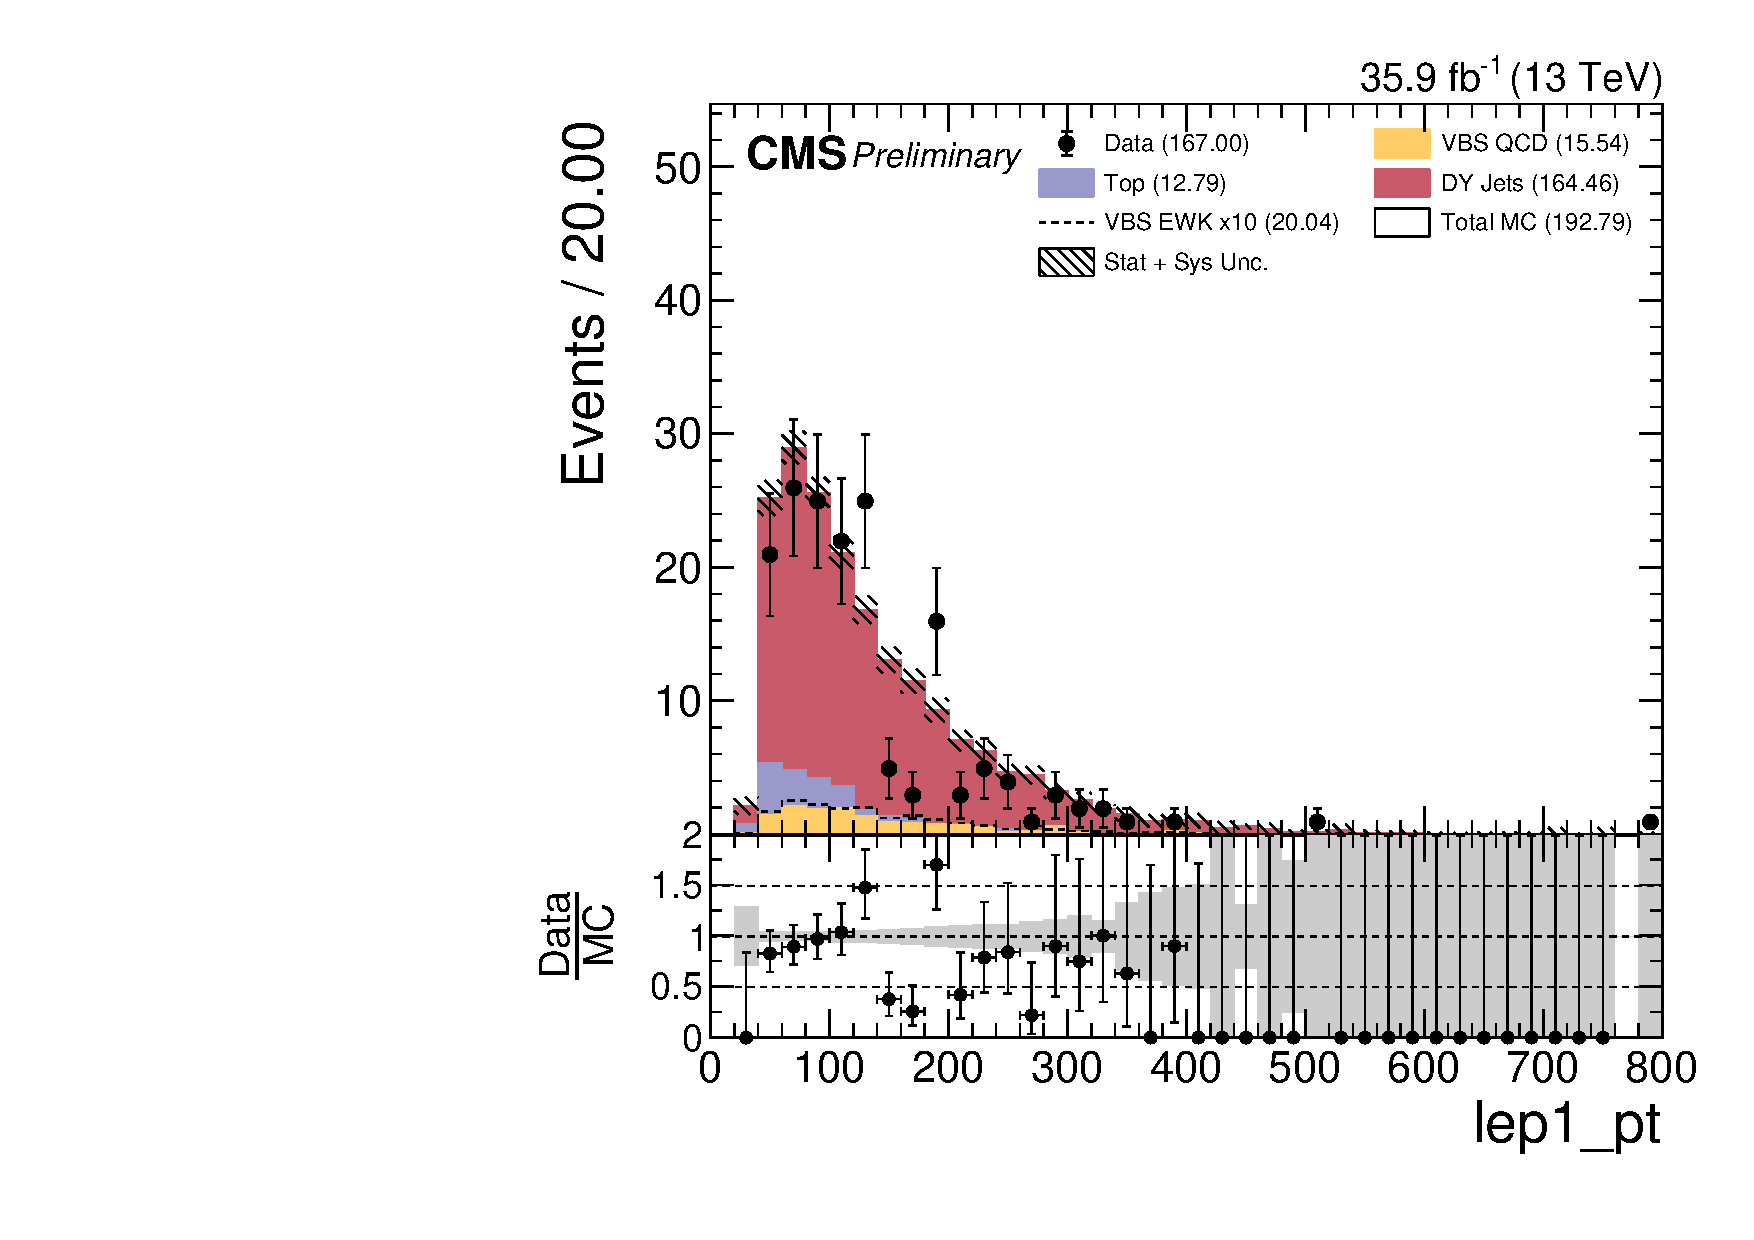
\includegraphics[width=0.30\textwidth]{analysis_plots/2016_zv/cr_vjets_e/lep1_pt.pdf}
  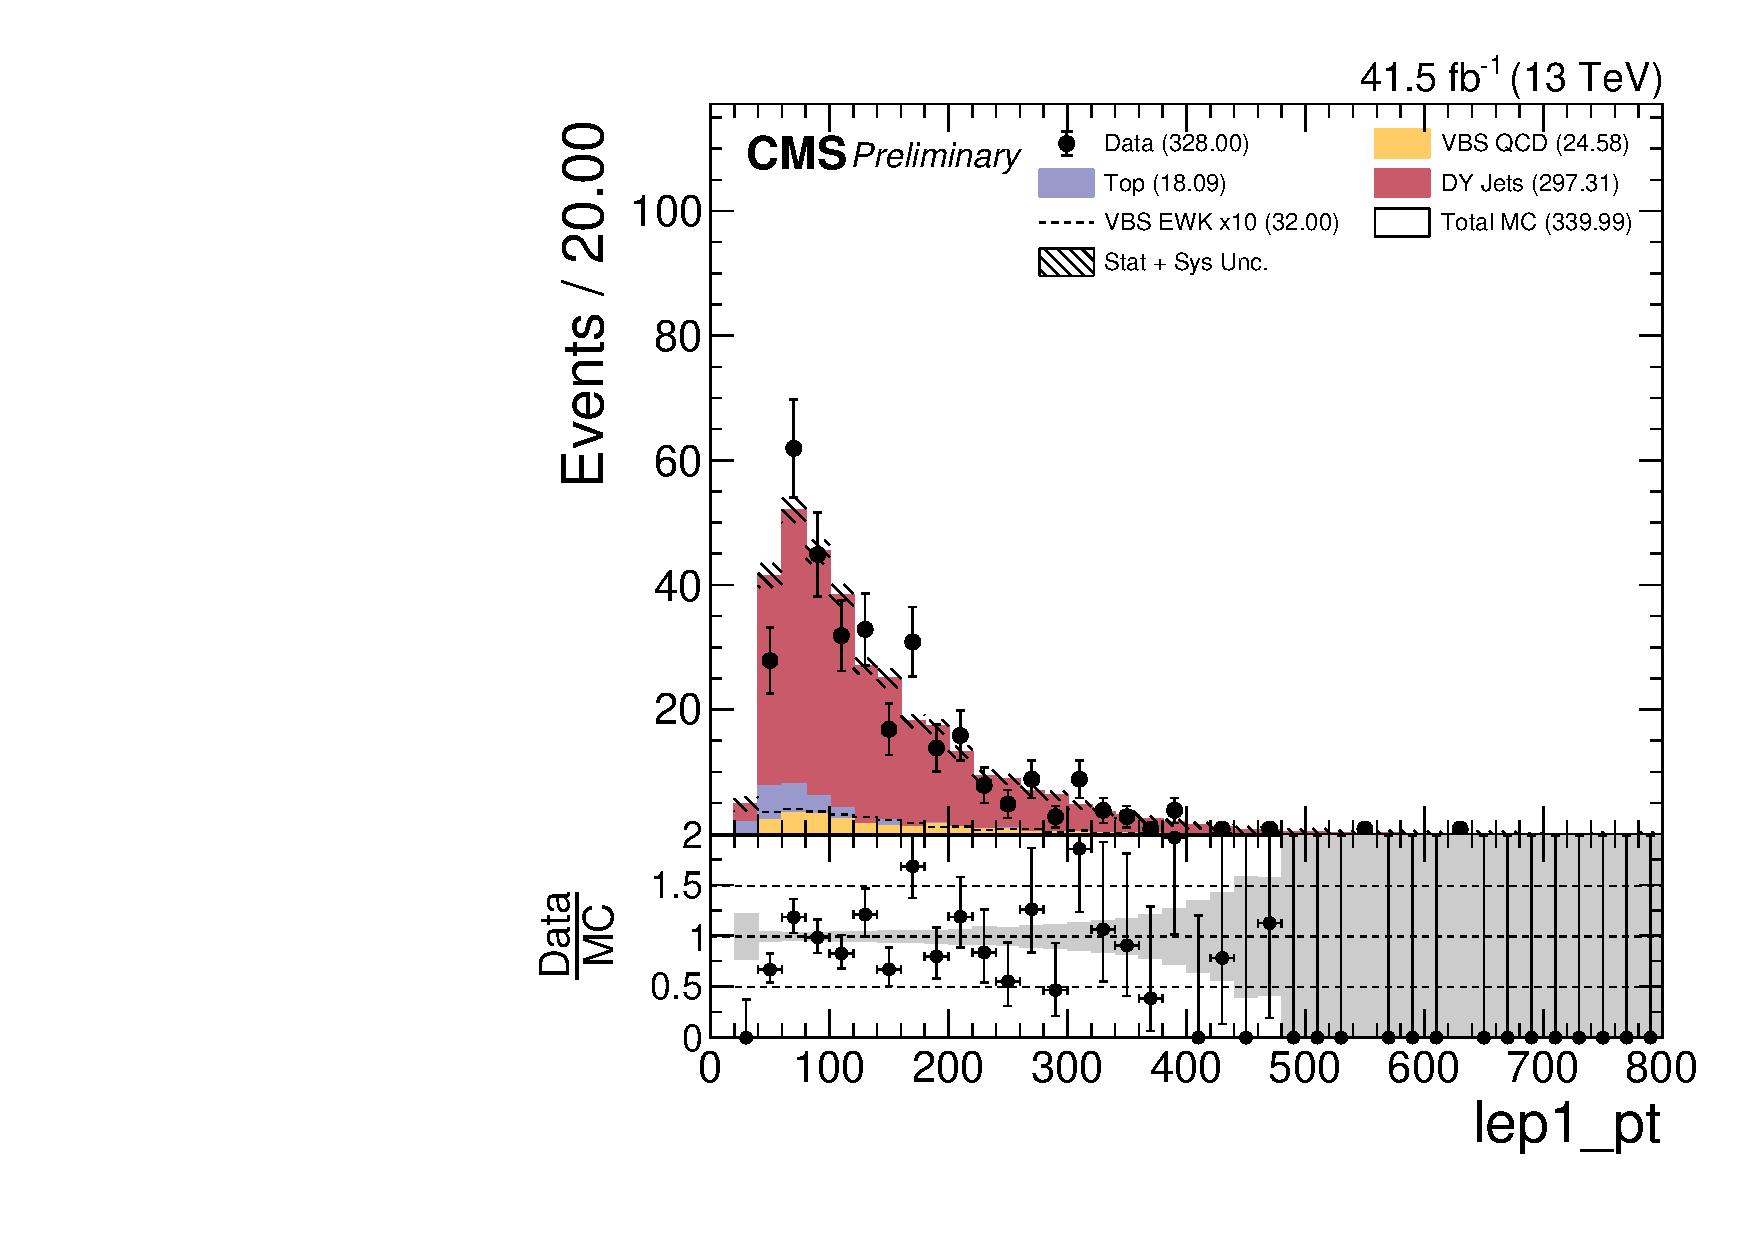
\includegraphics[width=0.30\textwidth]{analysis_plots/2017_zv/cr_vjets_e/lep1_pt.pdf}
  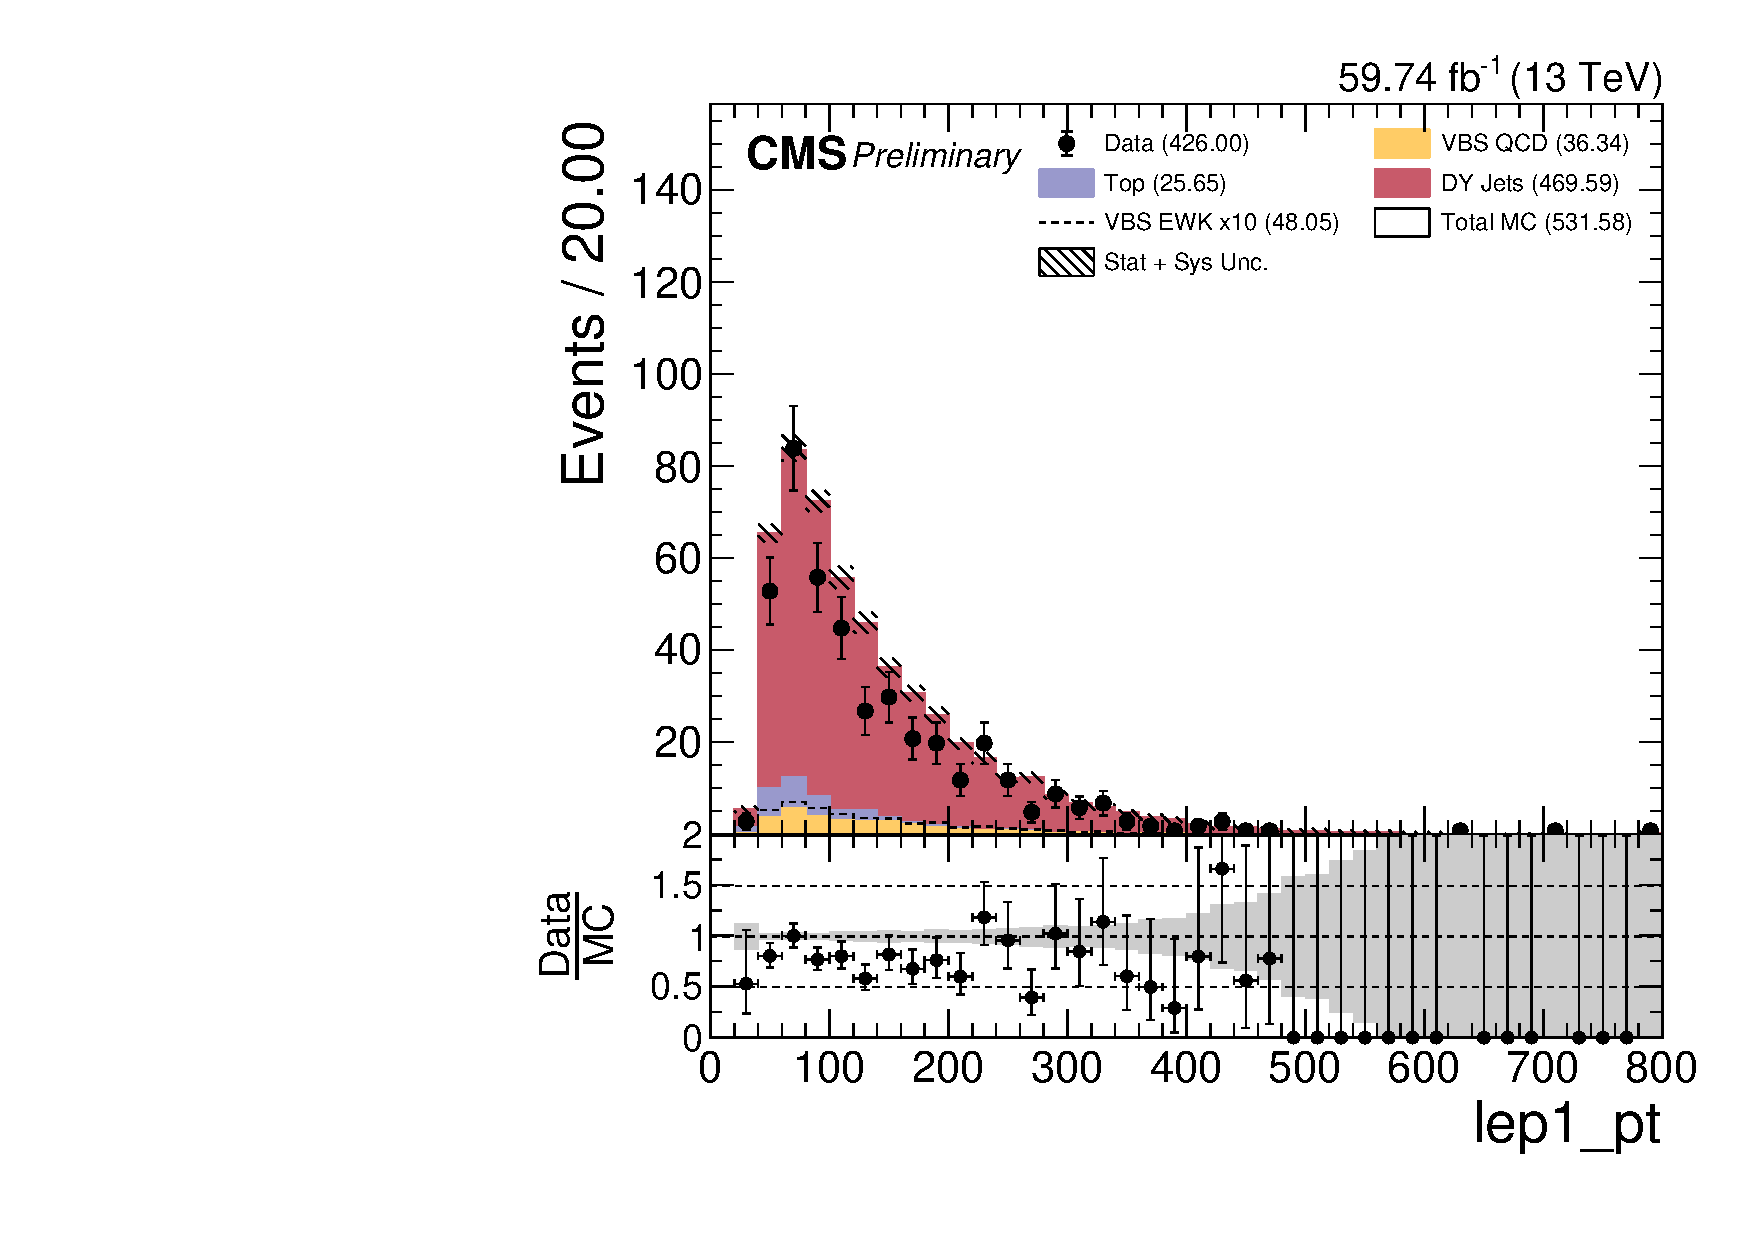
\includegraphics[width=0.30\textwidth]{analysis_plots/2018_zv/cr_vjets_e/lep1_pt.pdf} \\
  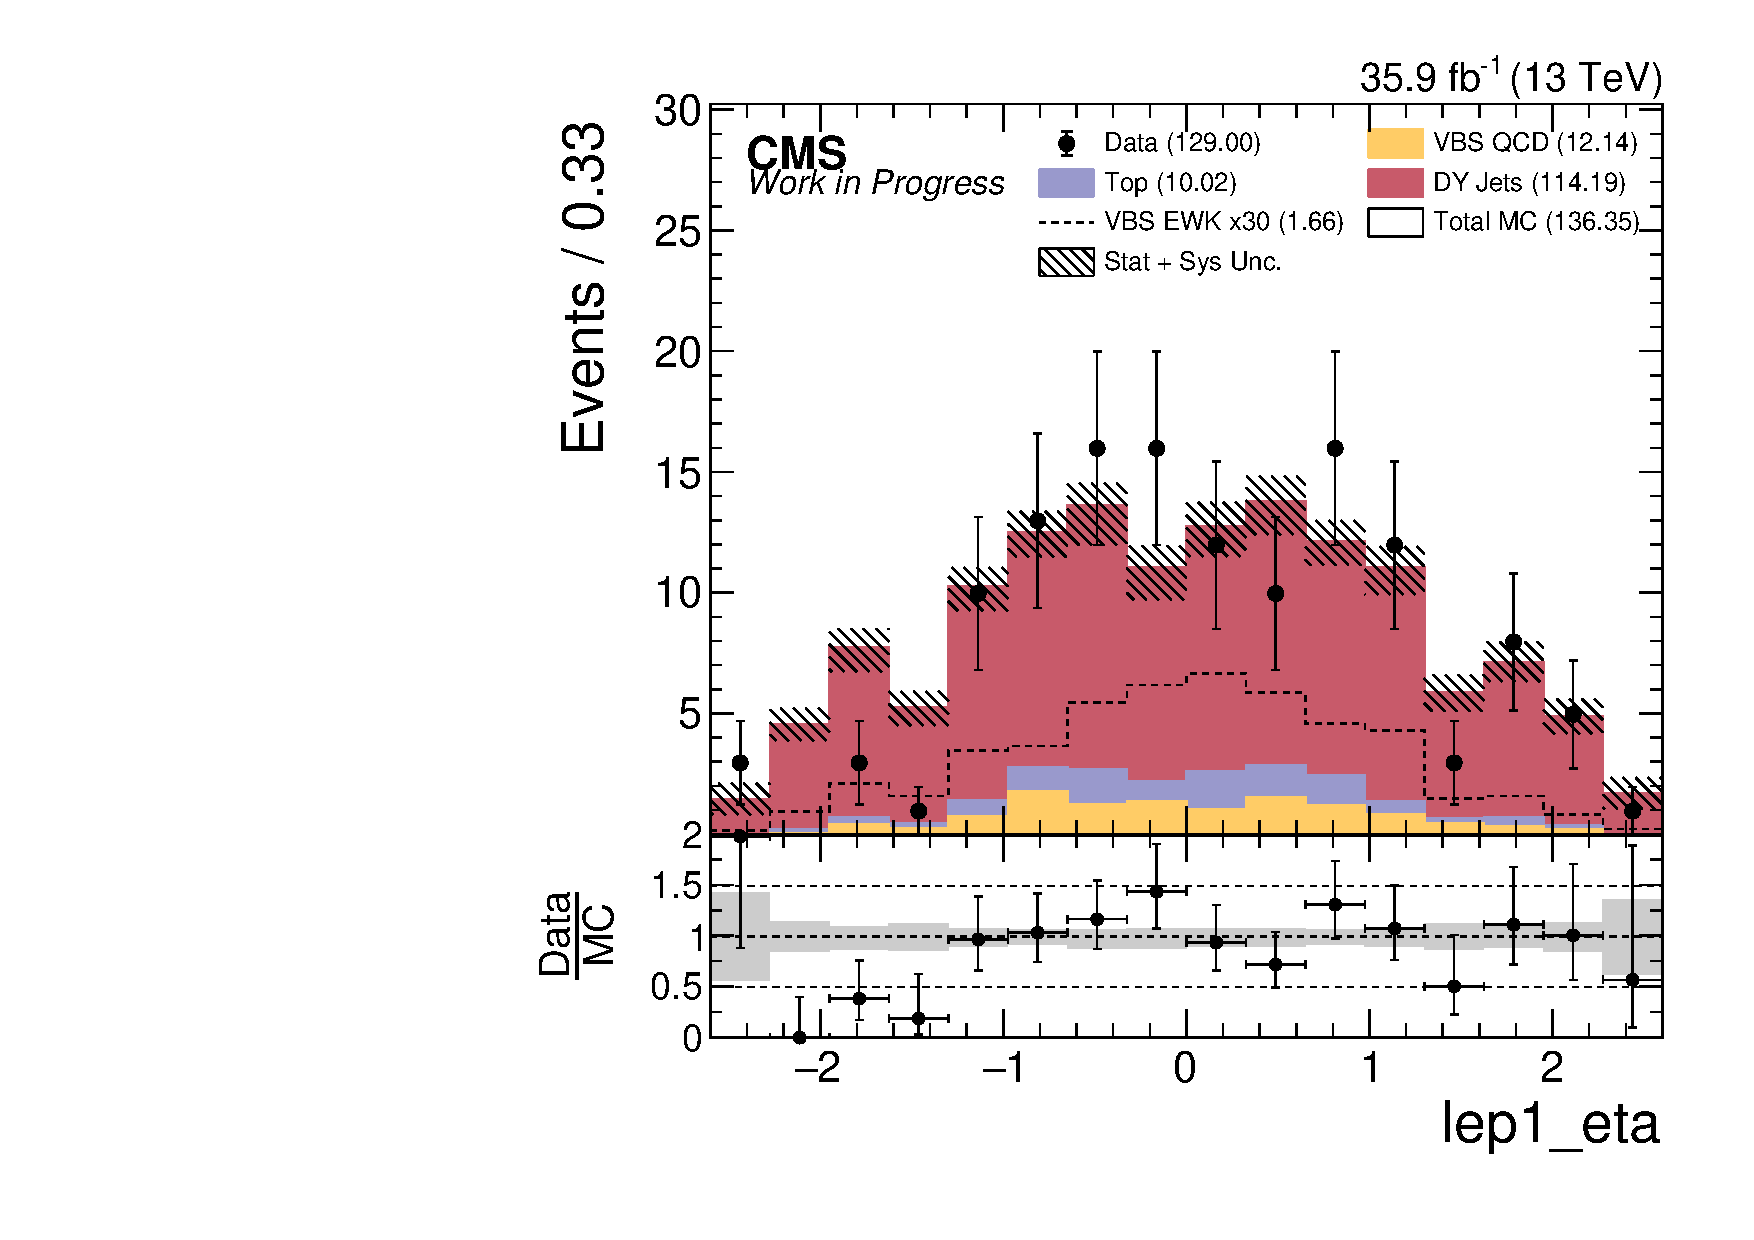
\includegraphics[width=0.30\textwidth]{analysis_plots/2016_zv/cr_vjets_e/lep1_eta.pdf}
  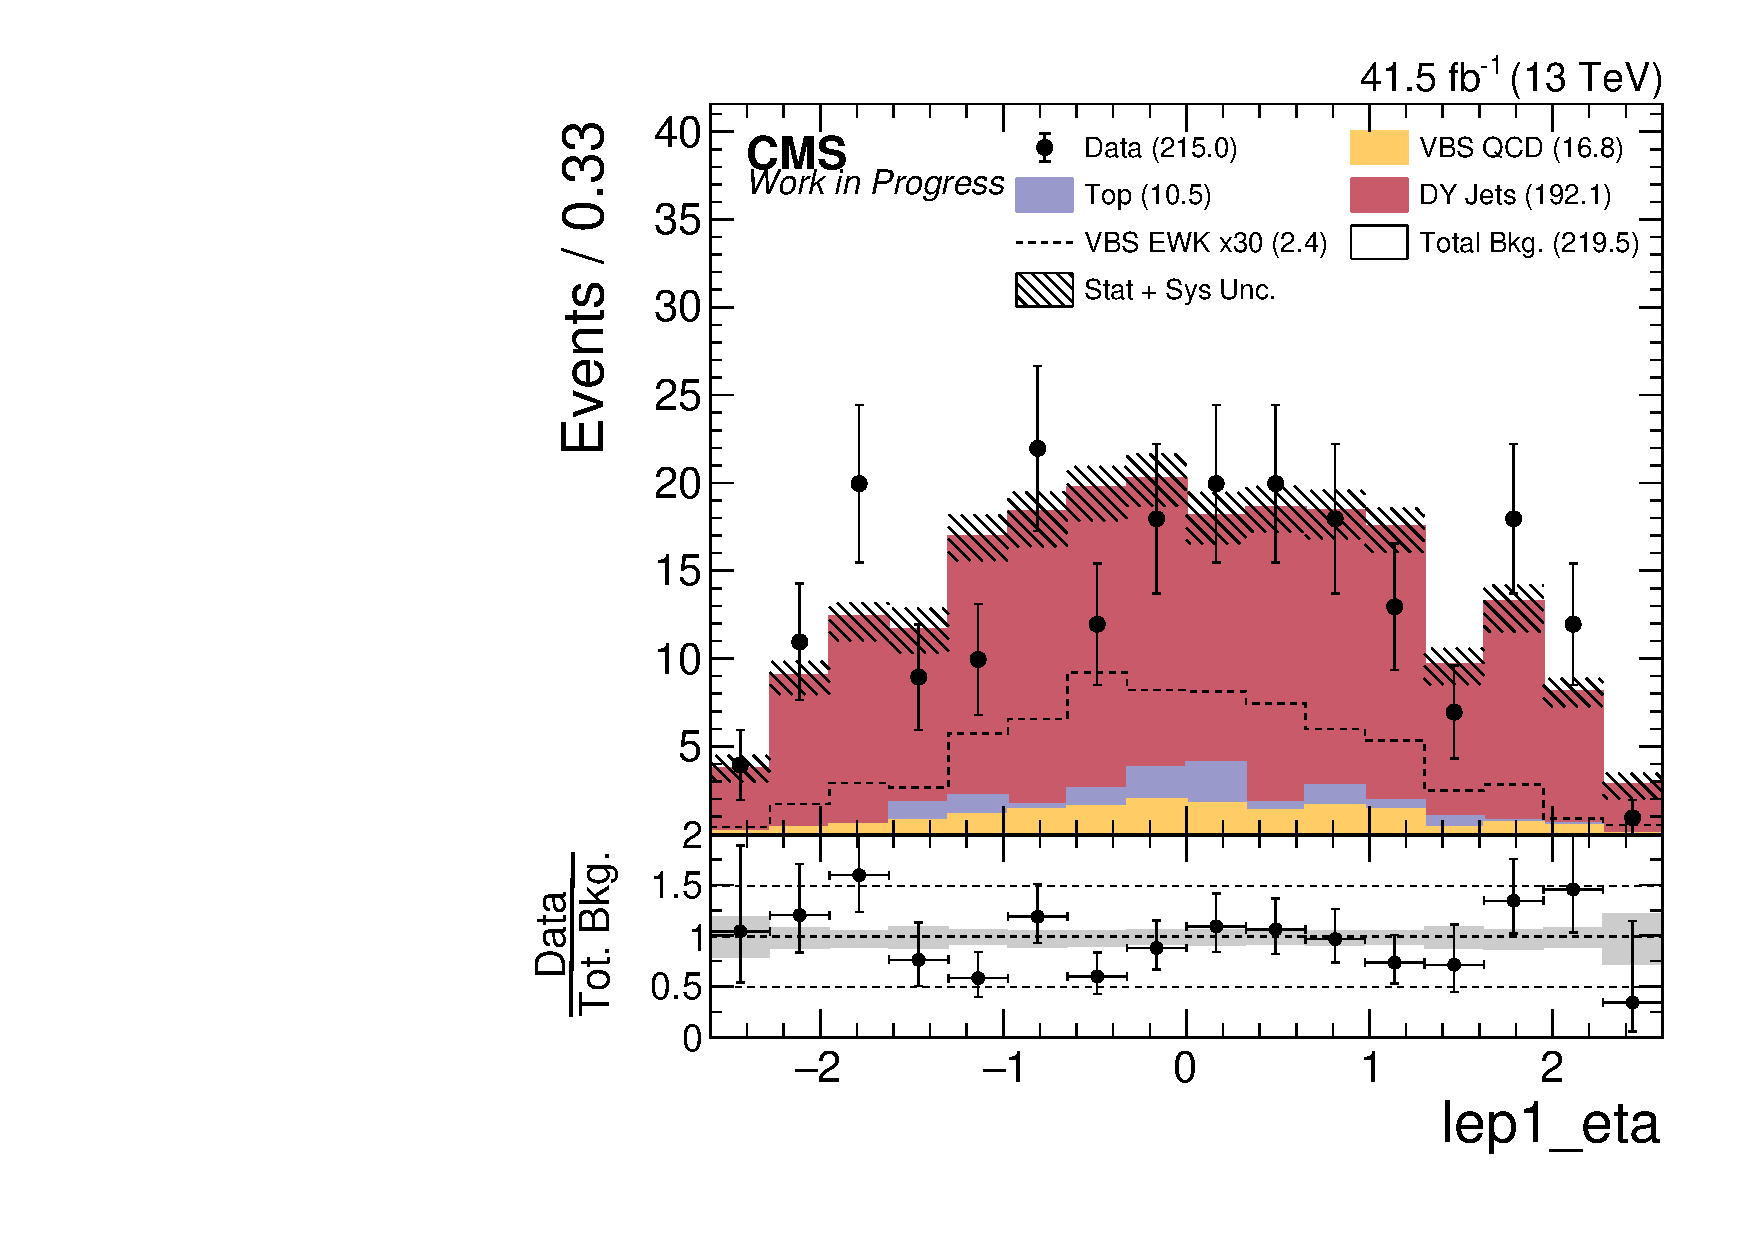
\includegraphics[width=0.30\textwidth]{analysis_plots/2017_zv/cr_vjets_e/lep1_eta.pdf}
  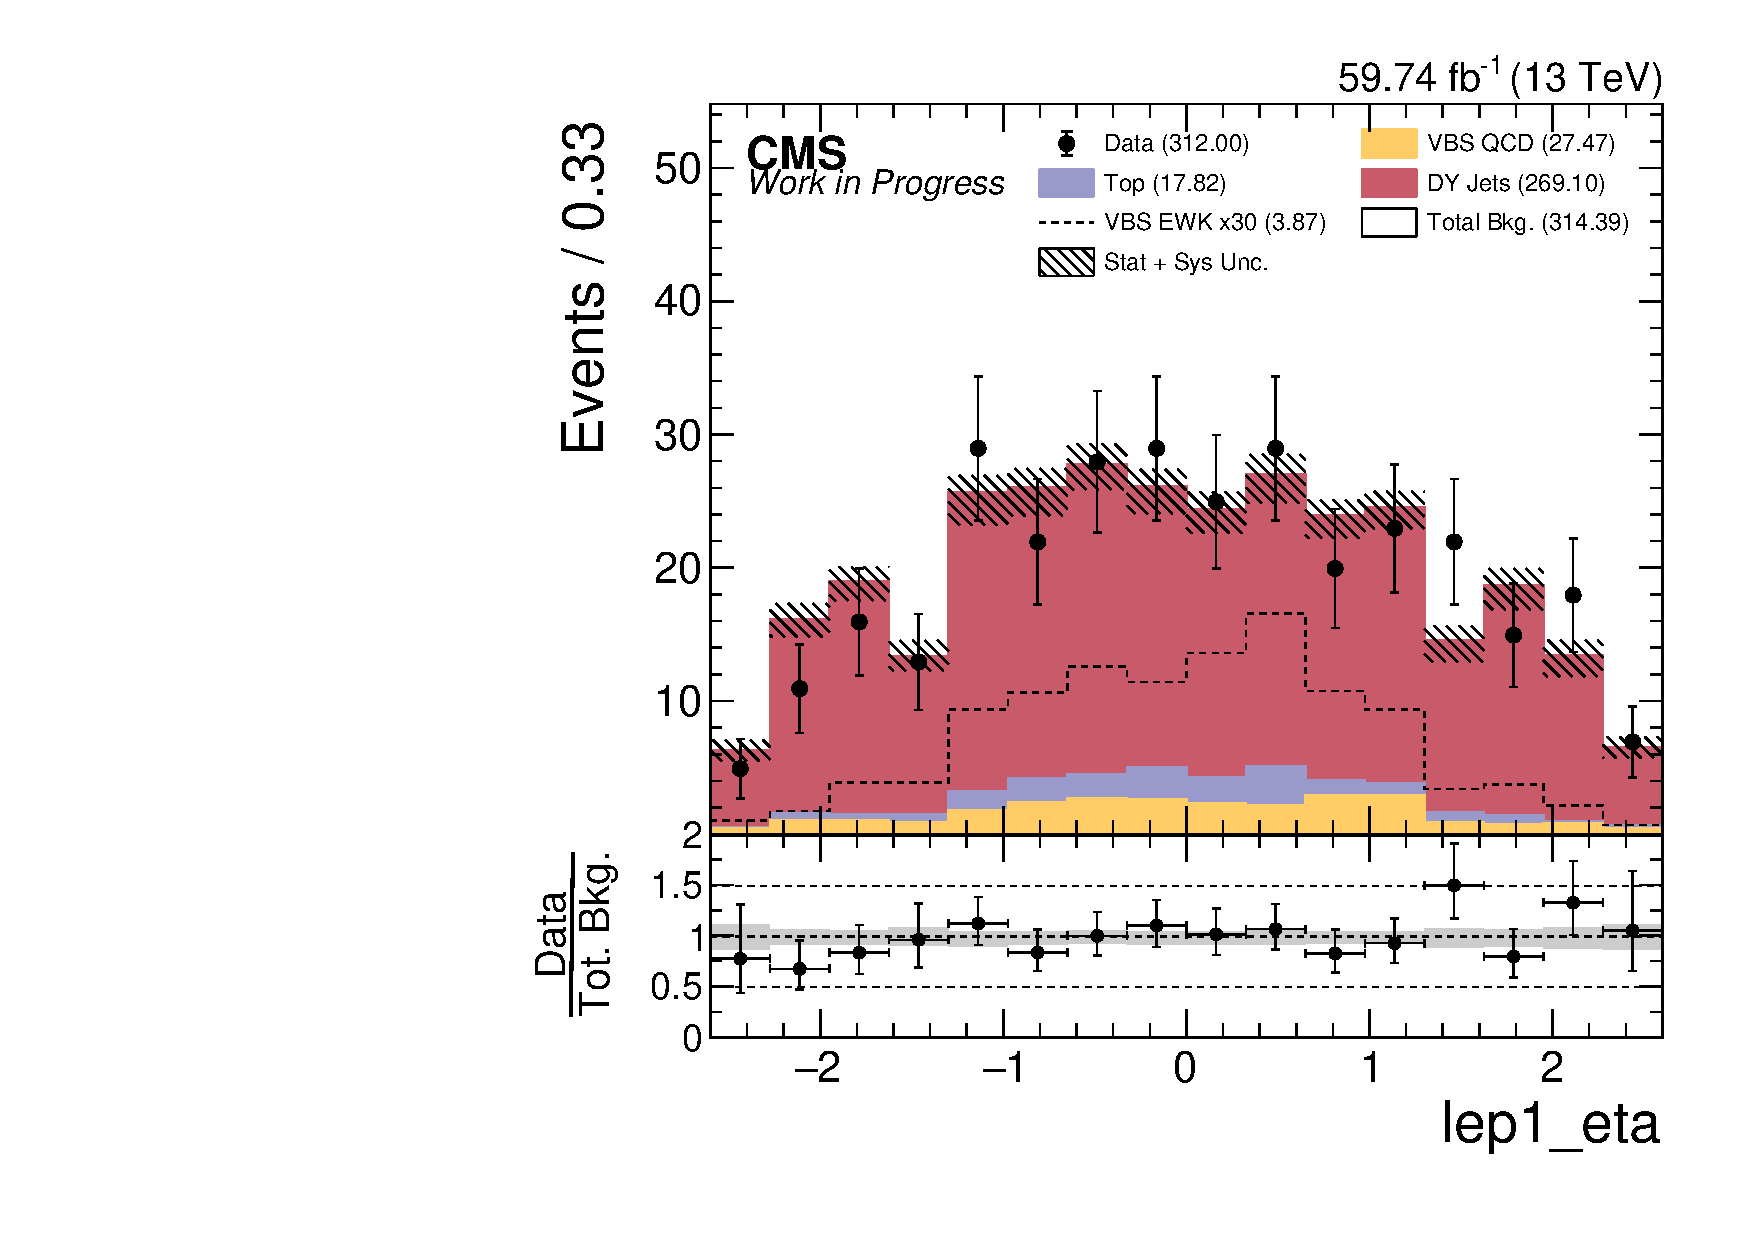
\includegraphics[width=0.30\textwidth]{analysis_plots/2018_zv/cr_vjets_e/lep1_eta.pdf} \\
  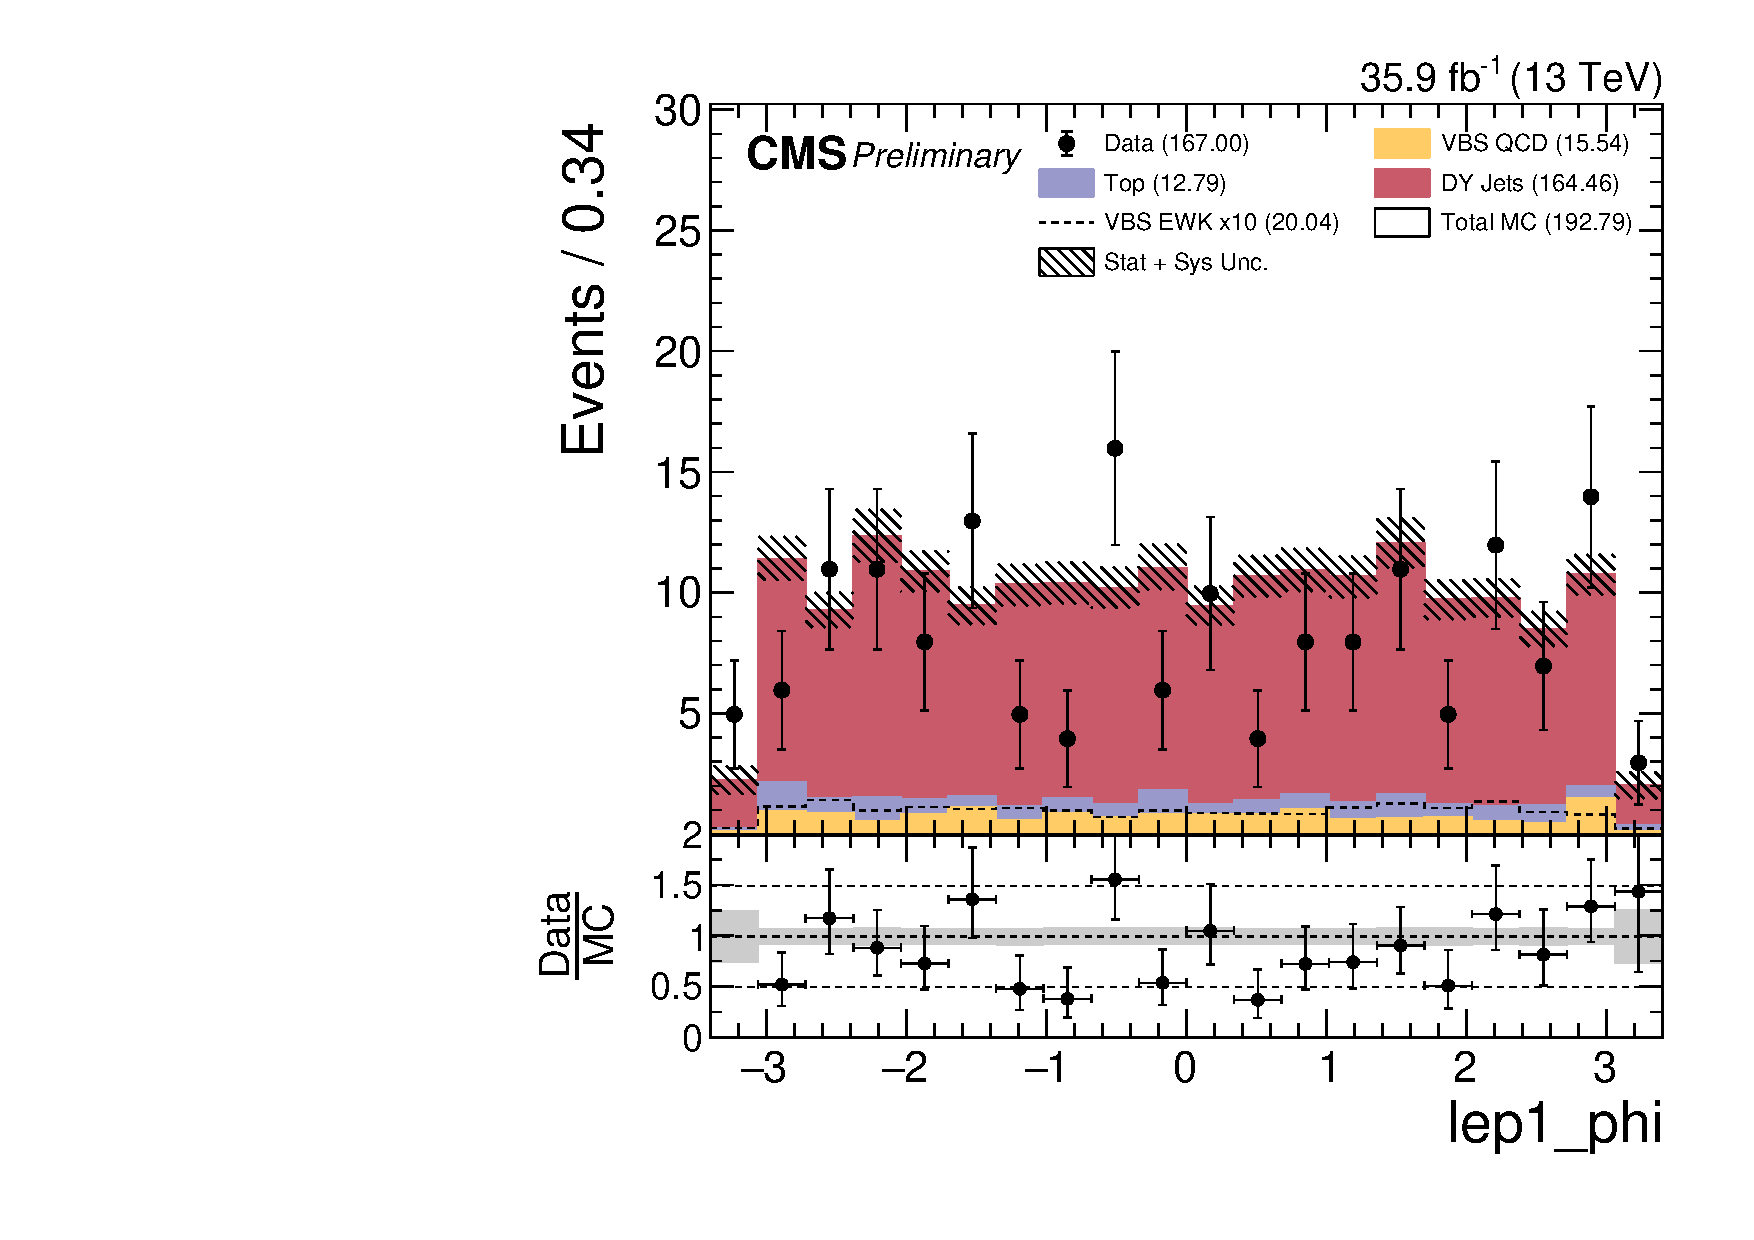
\includegraphics[width=0.30\textwidth]{analysis_plots/2016_zv/cr_vjets_e/lep1_phi.pdf}
  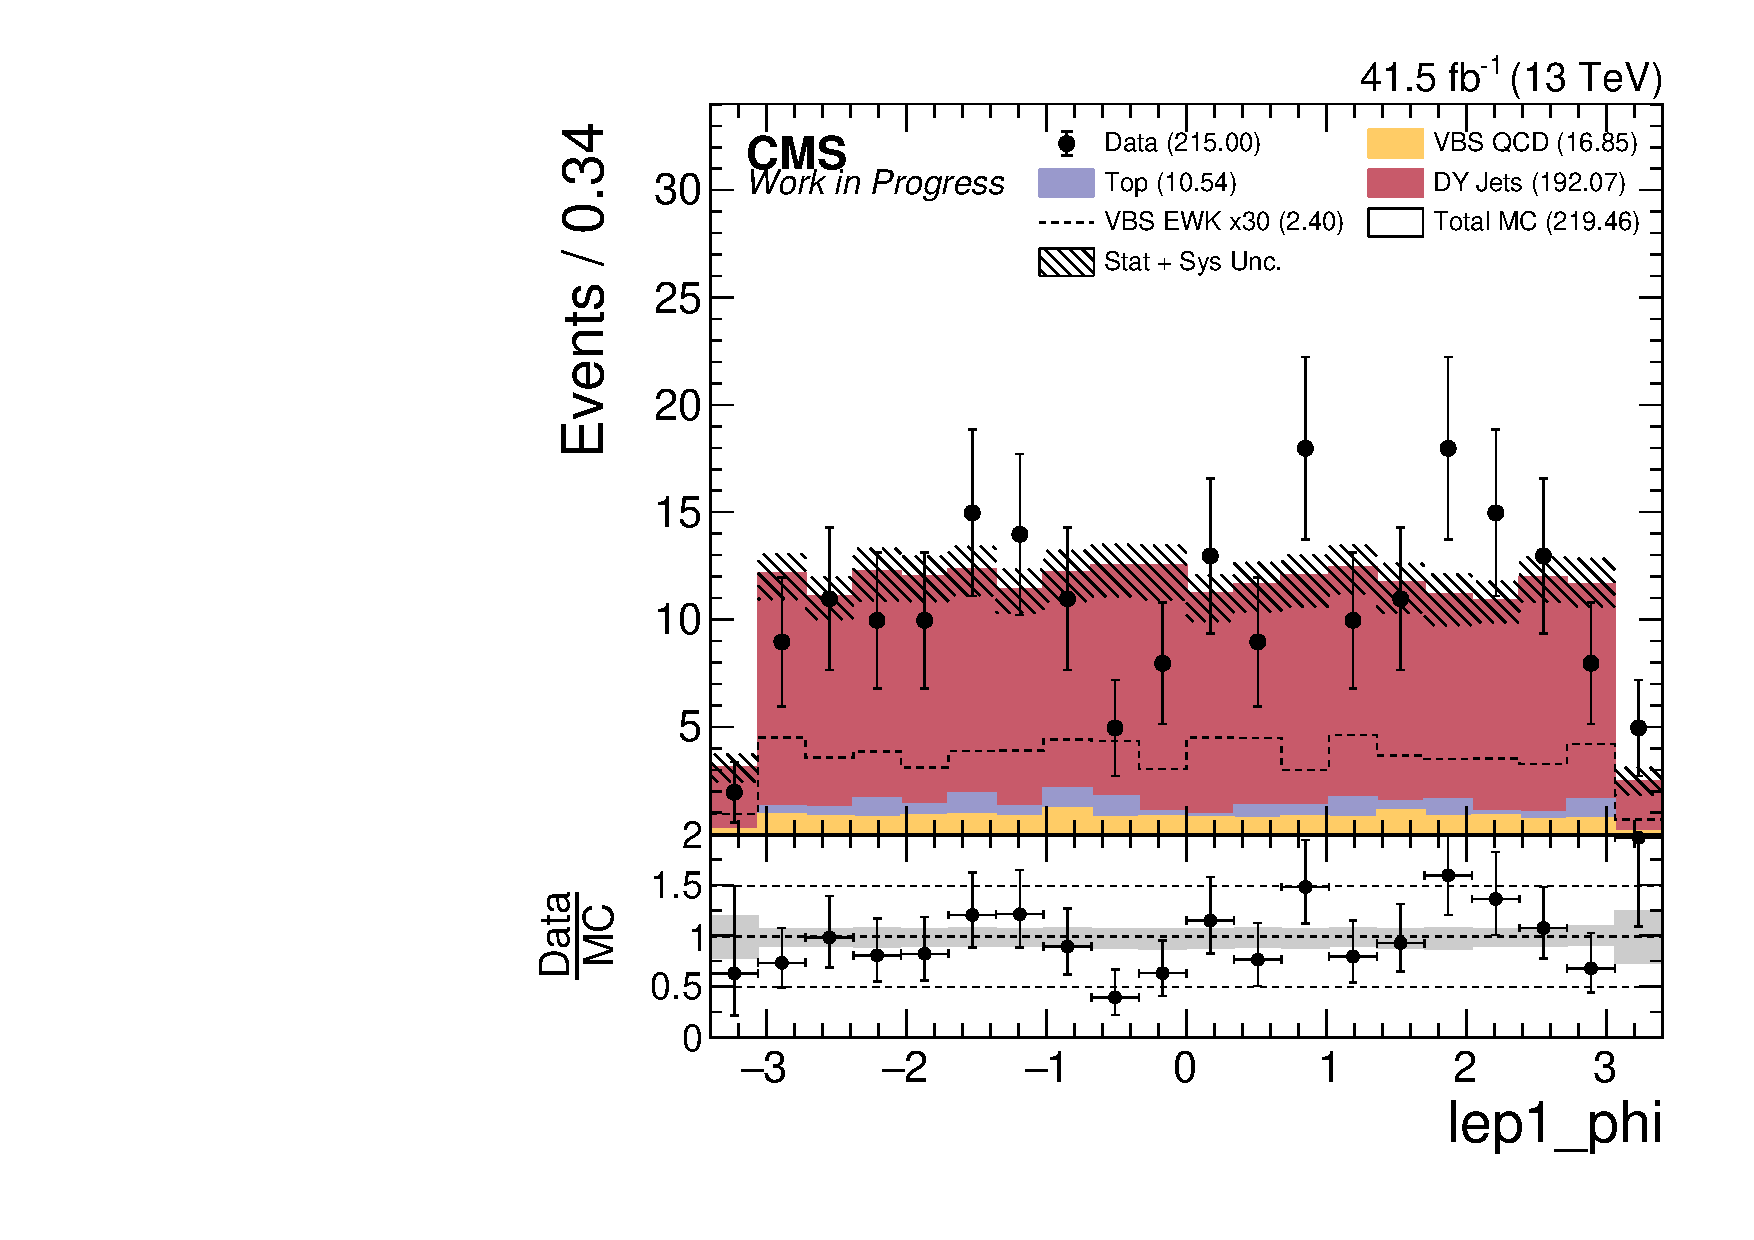
\includegraphics[width=0.30\textwidth]{analysis_plots/2017_zv/cr_vjets_e/lep1_phi.pdf}
  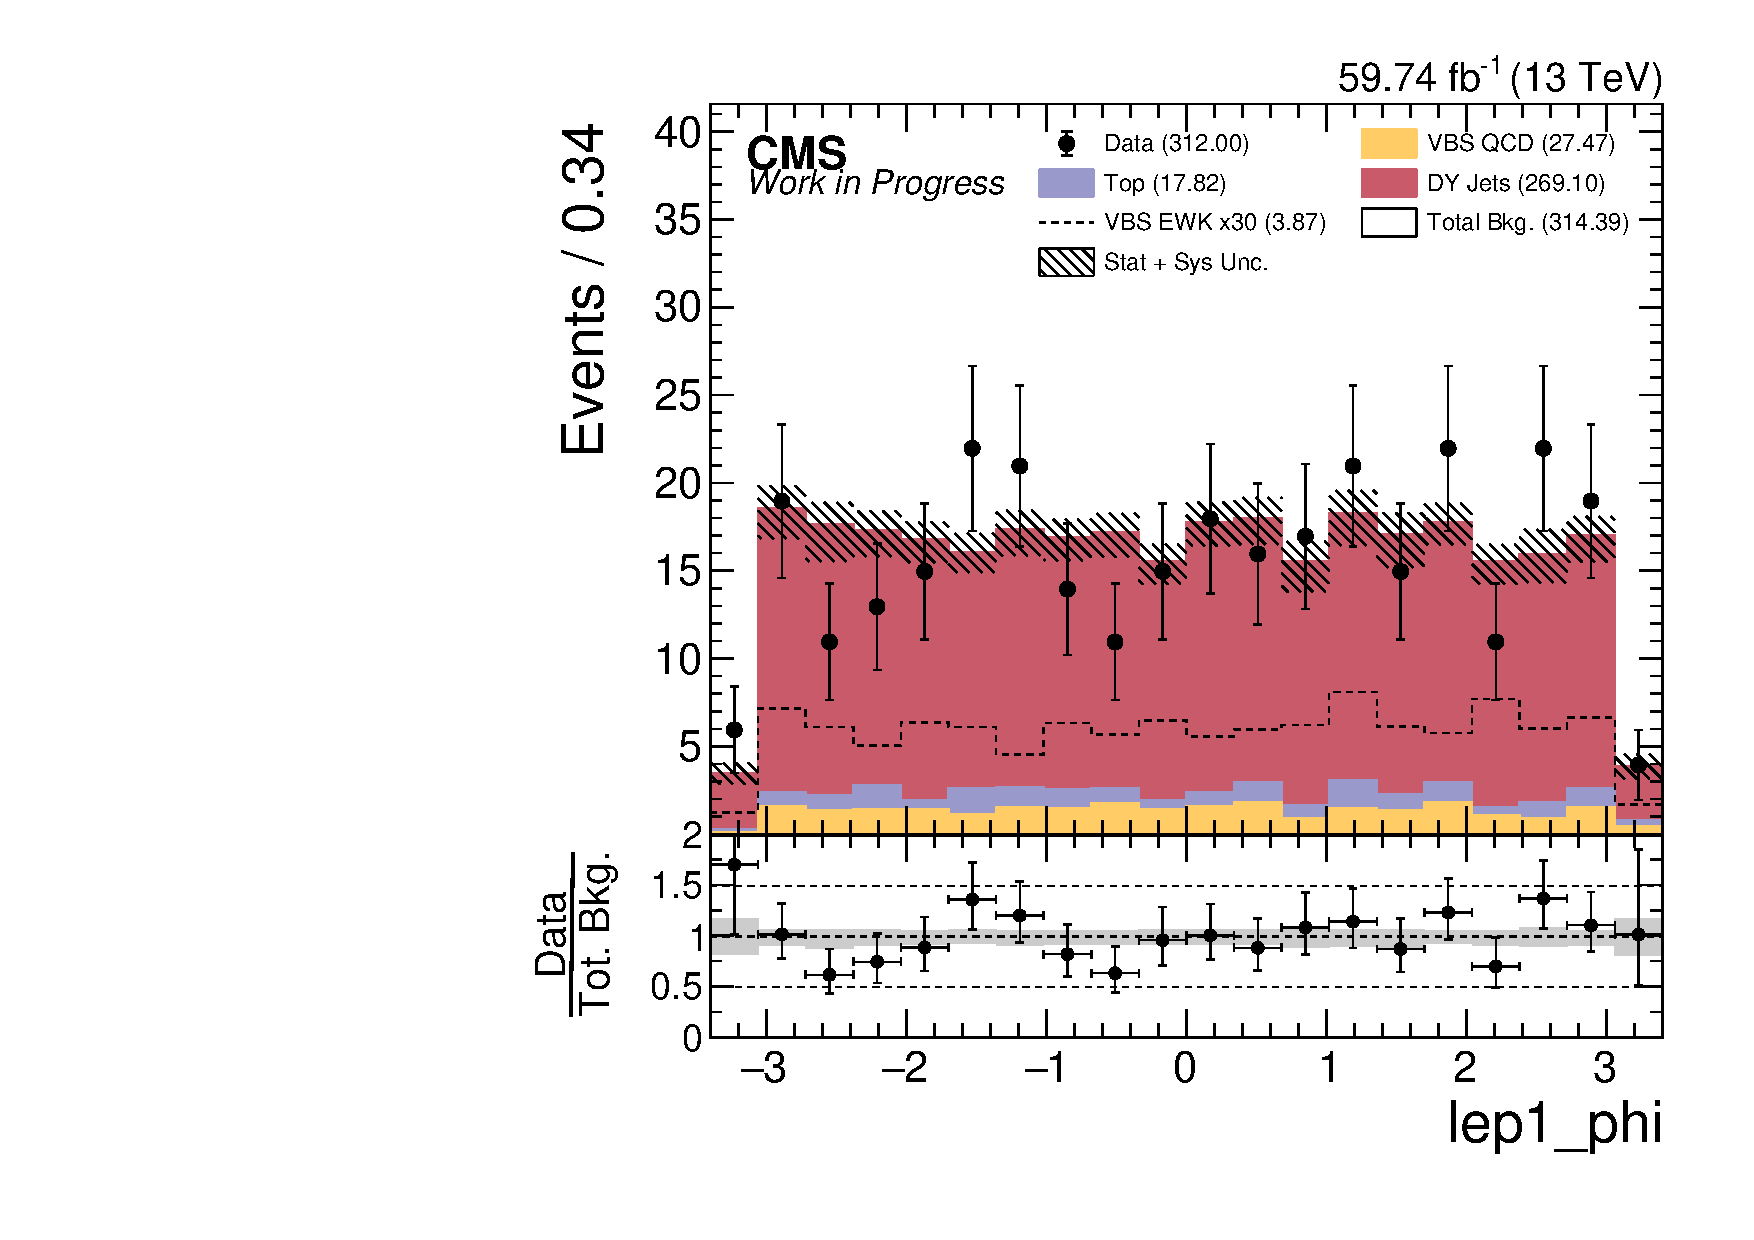
\includegraphics[width=0.30\textwidth]{analysis_plots/2018_zv/cr_vjets_e/lep1_phi.pdf} \\
  \caption[DY+Jets Control Region: Leading electron kinematics in Boosted ZV Channel]%
  {DY+Jets Control Region: Leading electron kinematics in Boosted ZV Channel. From Left to Right: 2016,
    2017, and 2018. From Top to Bottom: \( p_T \), \( \eta \), \( \phi \).}%
  \label{fig:zv-cr-vjets-e-lep1-pt-eta-phi}
\end{figure}

\begin{figure}[!ht]
  \centering
  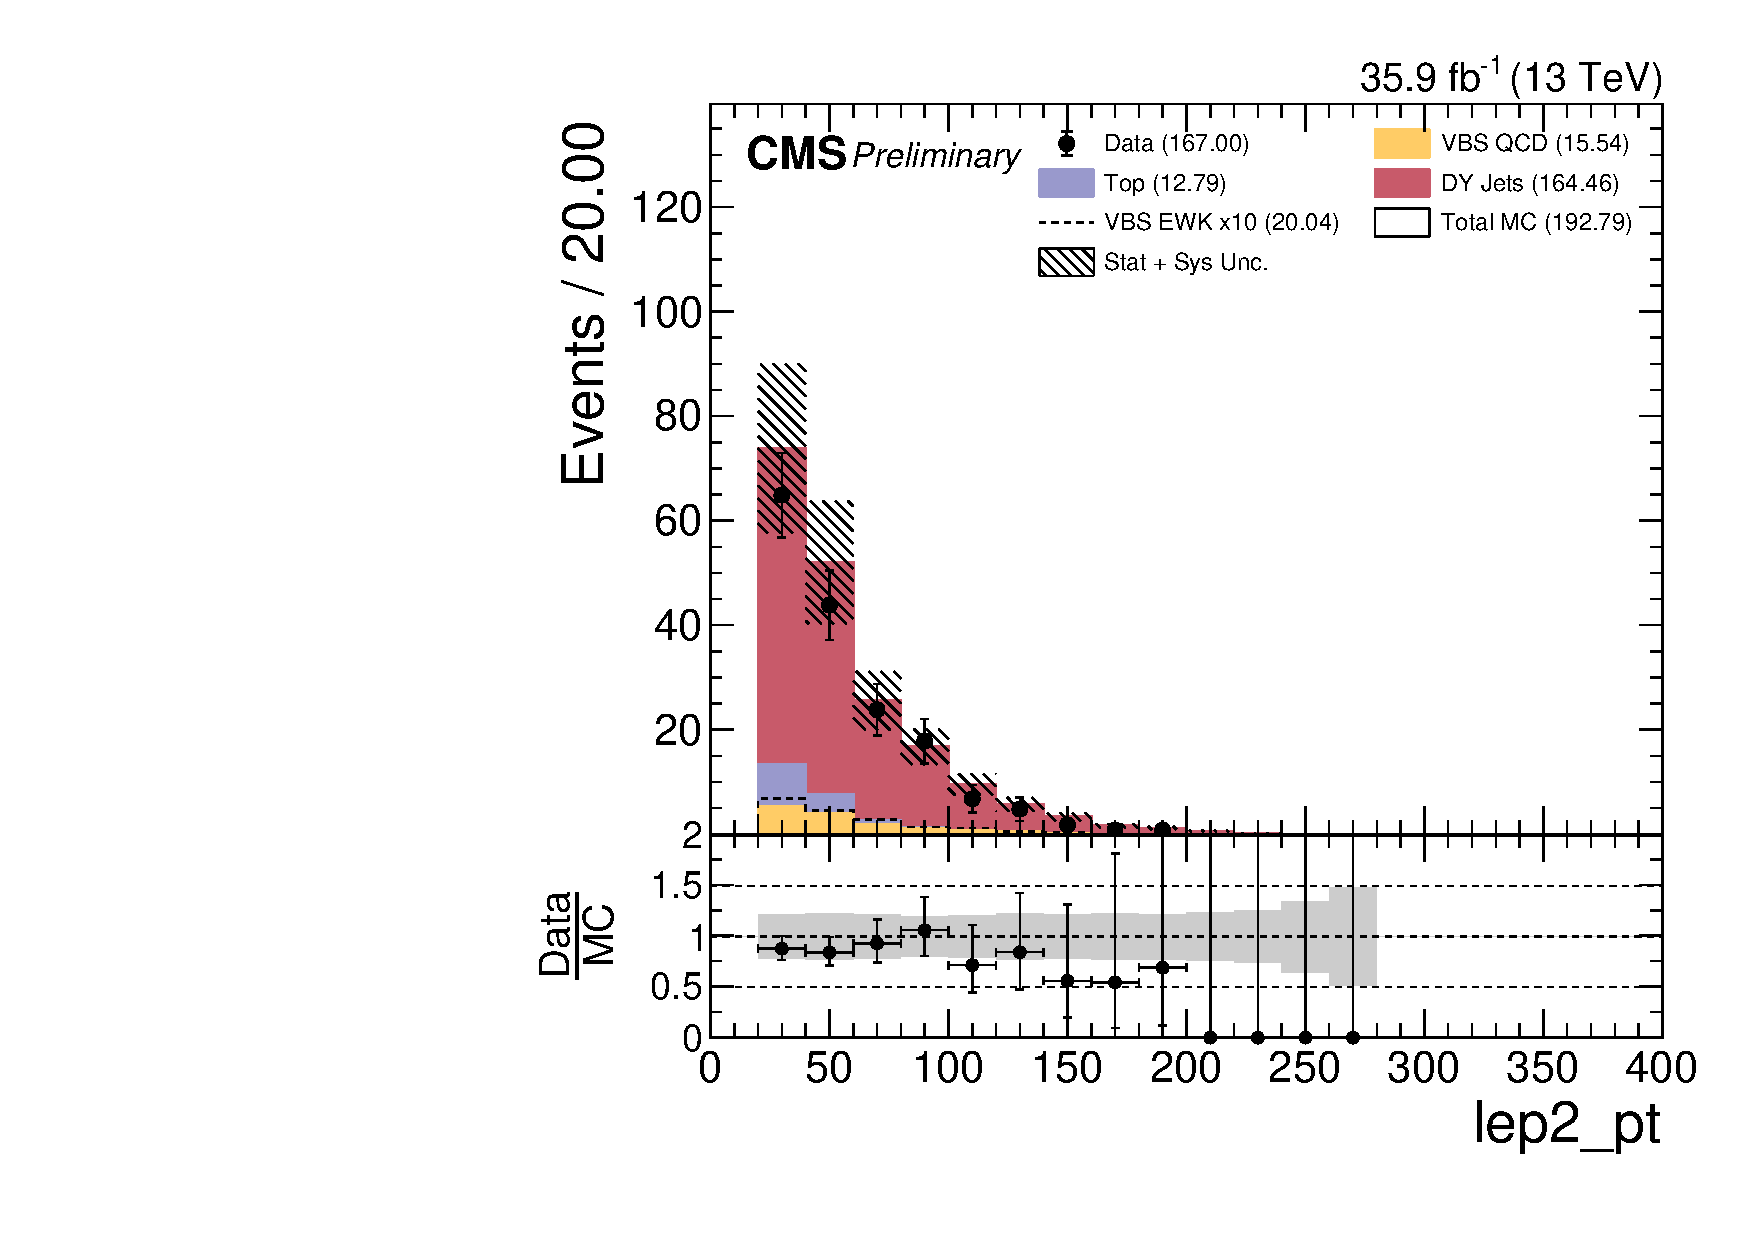
\includegraphics[width=0.30\textwidth]{analysis_plots/2016_zv/cr_vjets_e/lep2_pt.pdf}
  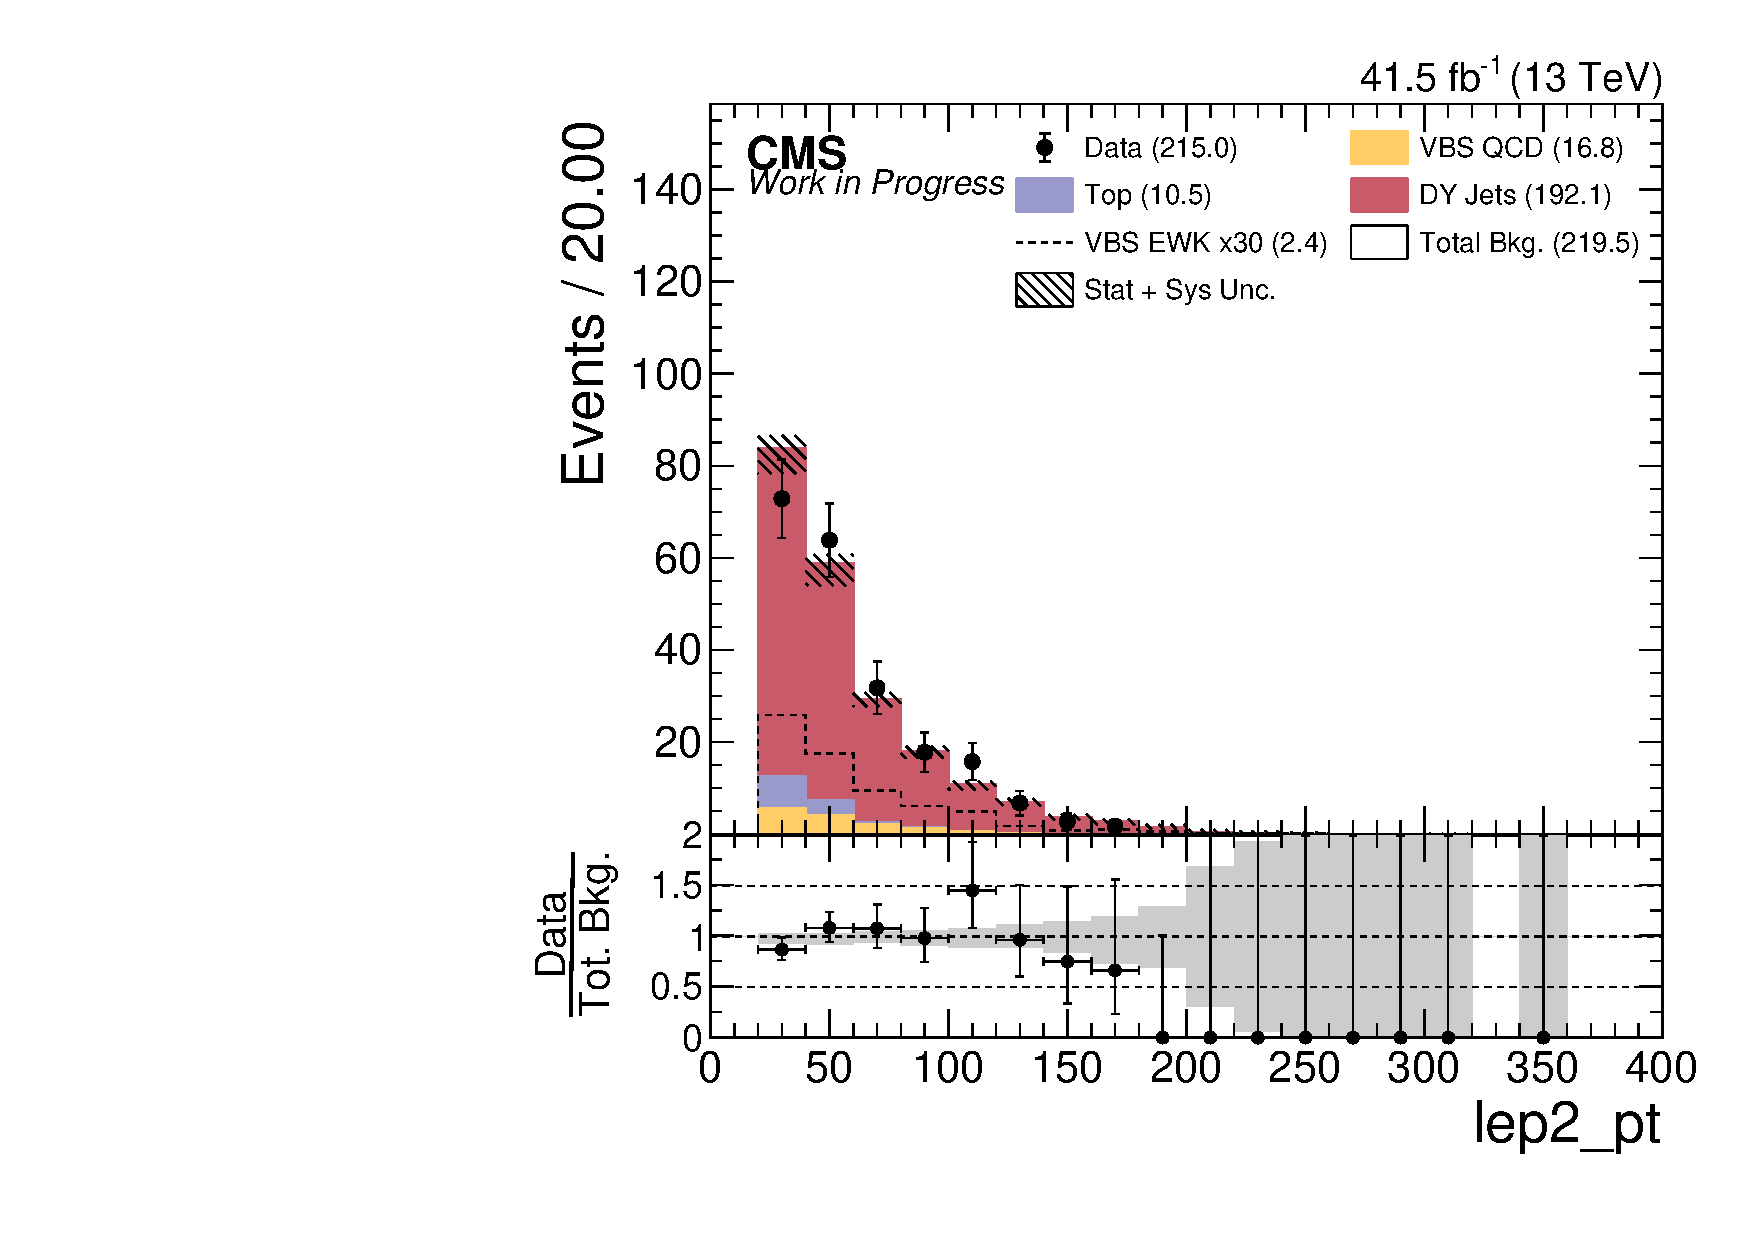
\includegraphics[width=0.30\textwidth]{analysis_plots/2017_zv/cr_vjets_e/lep2_pt.pdf}
  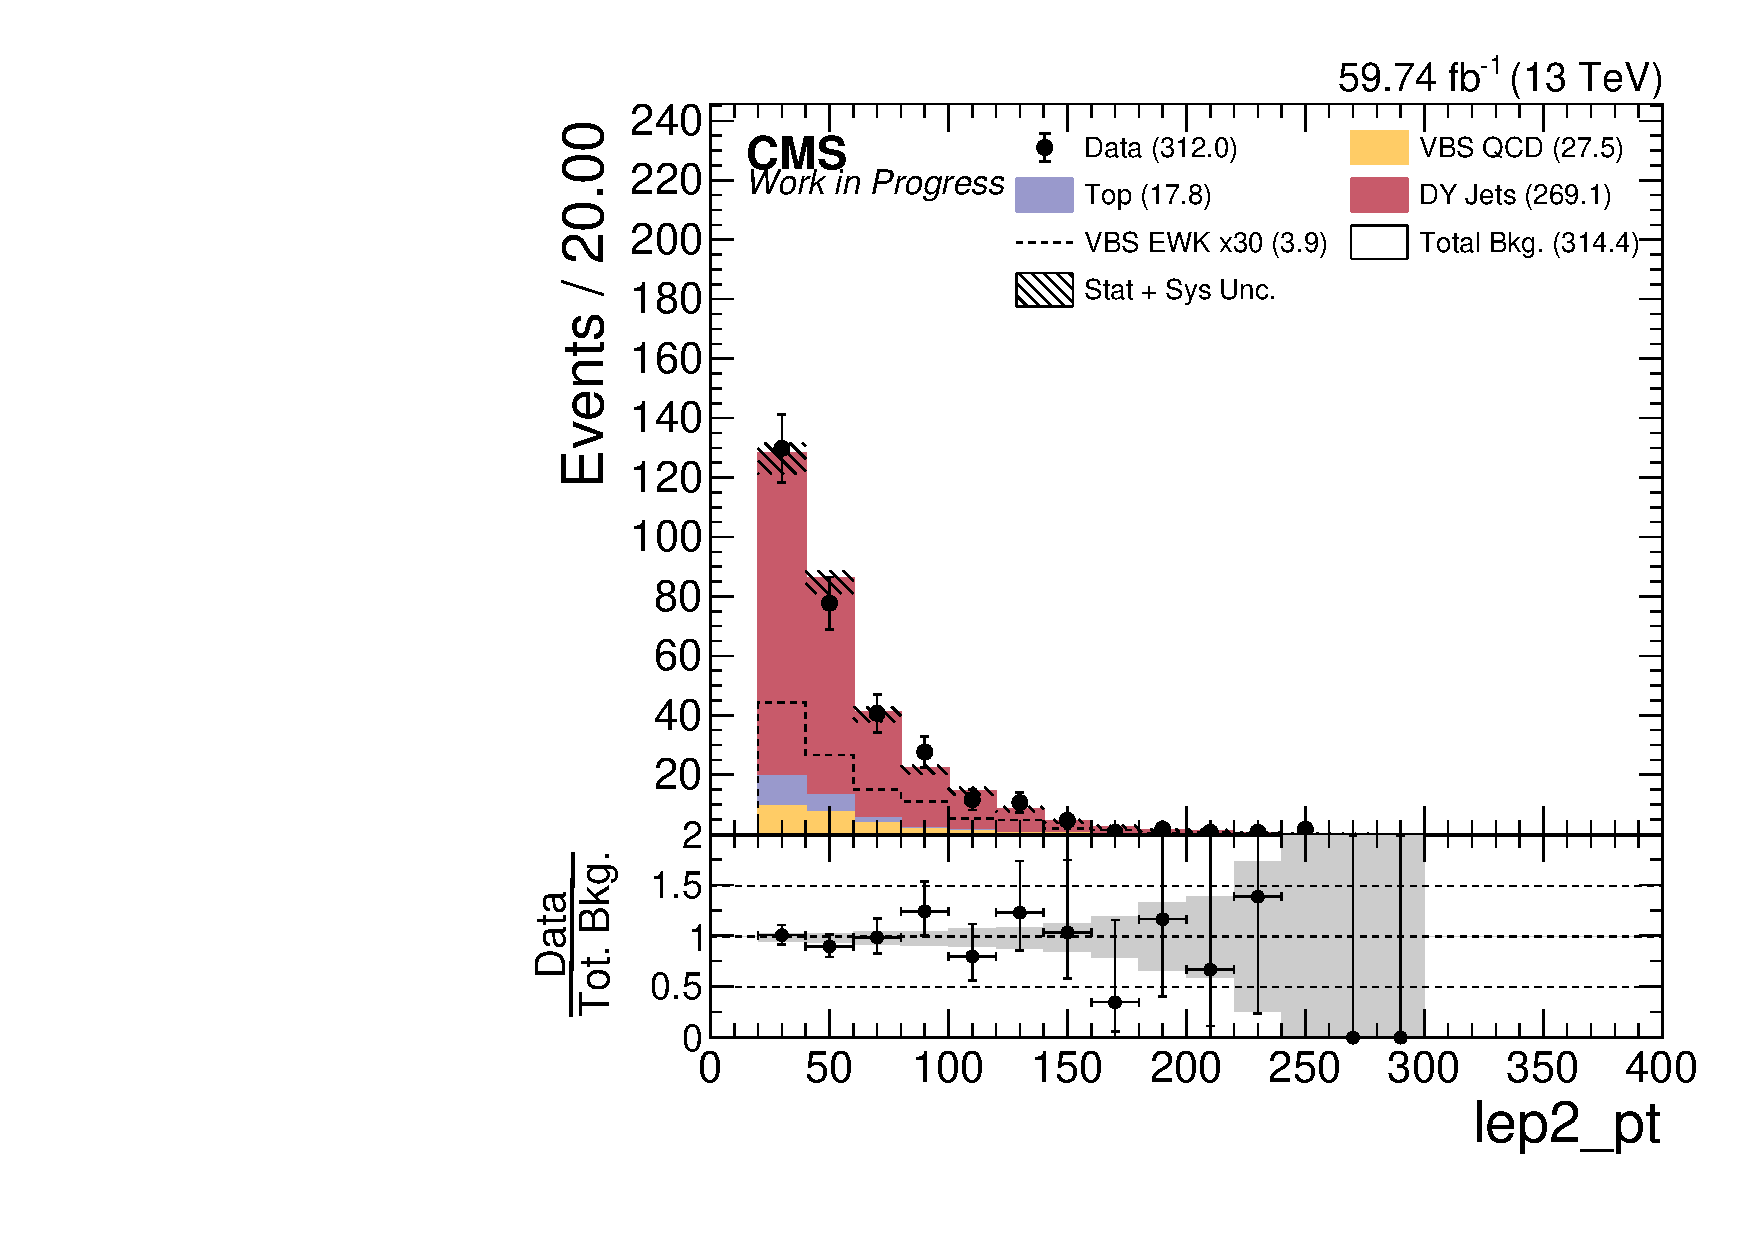
\includegraphics[width=0.30\textwidth]{analysis_plots/2018_zv/cr_vjets_e/lep2_pt.pdf} \\
  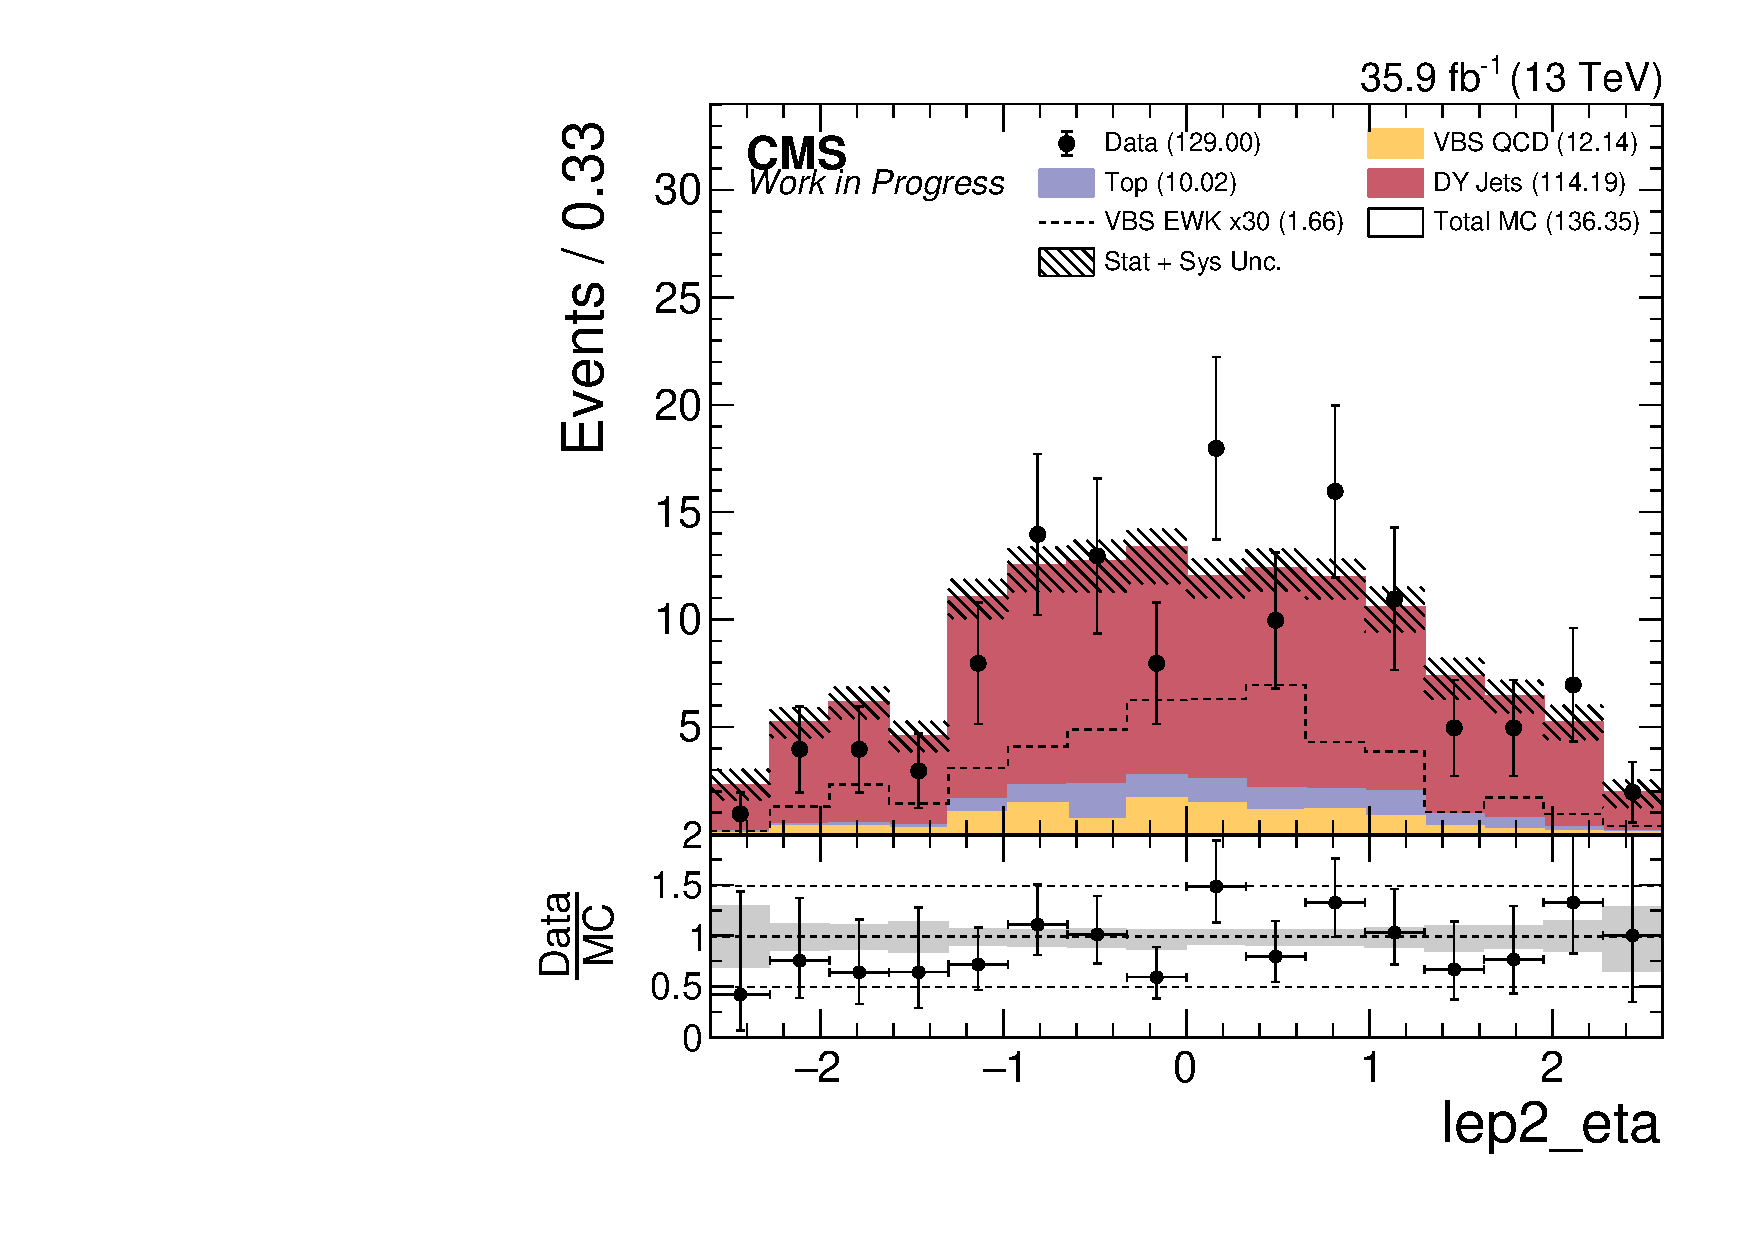
\includegraphics[width=0.30\textwidth]{analysis_plots/2016_zv/cr_vjets_e/lep2_eta.pdf}
  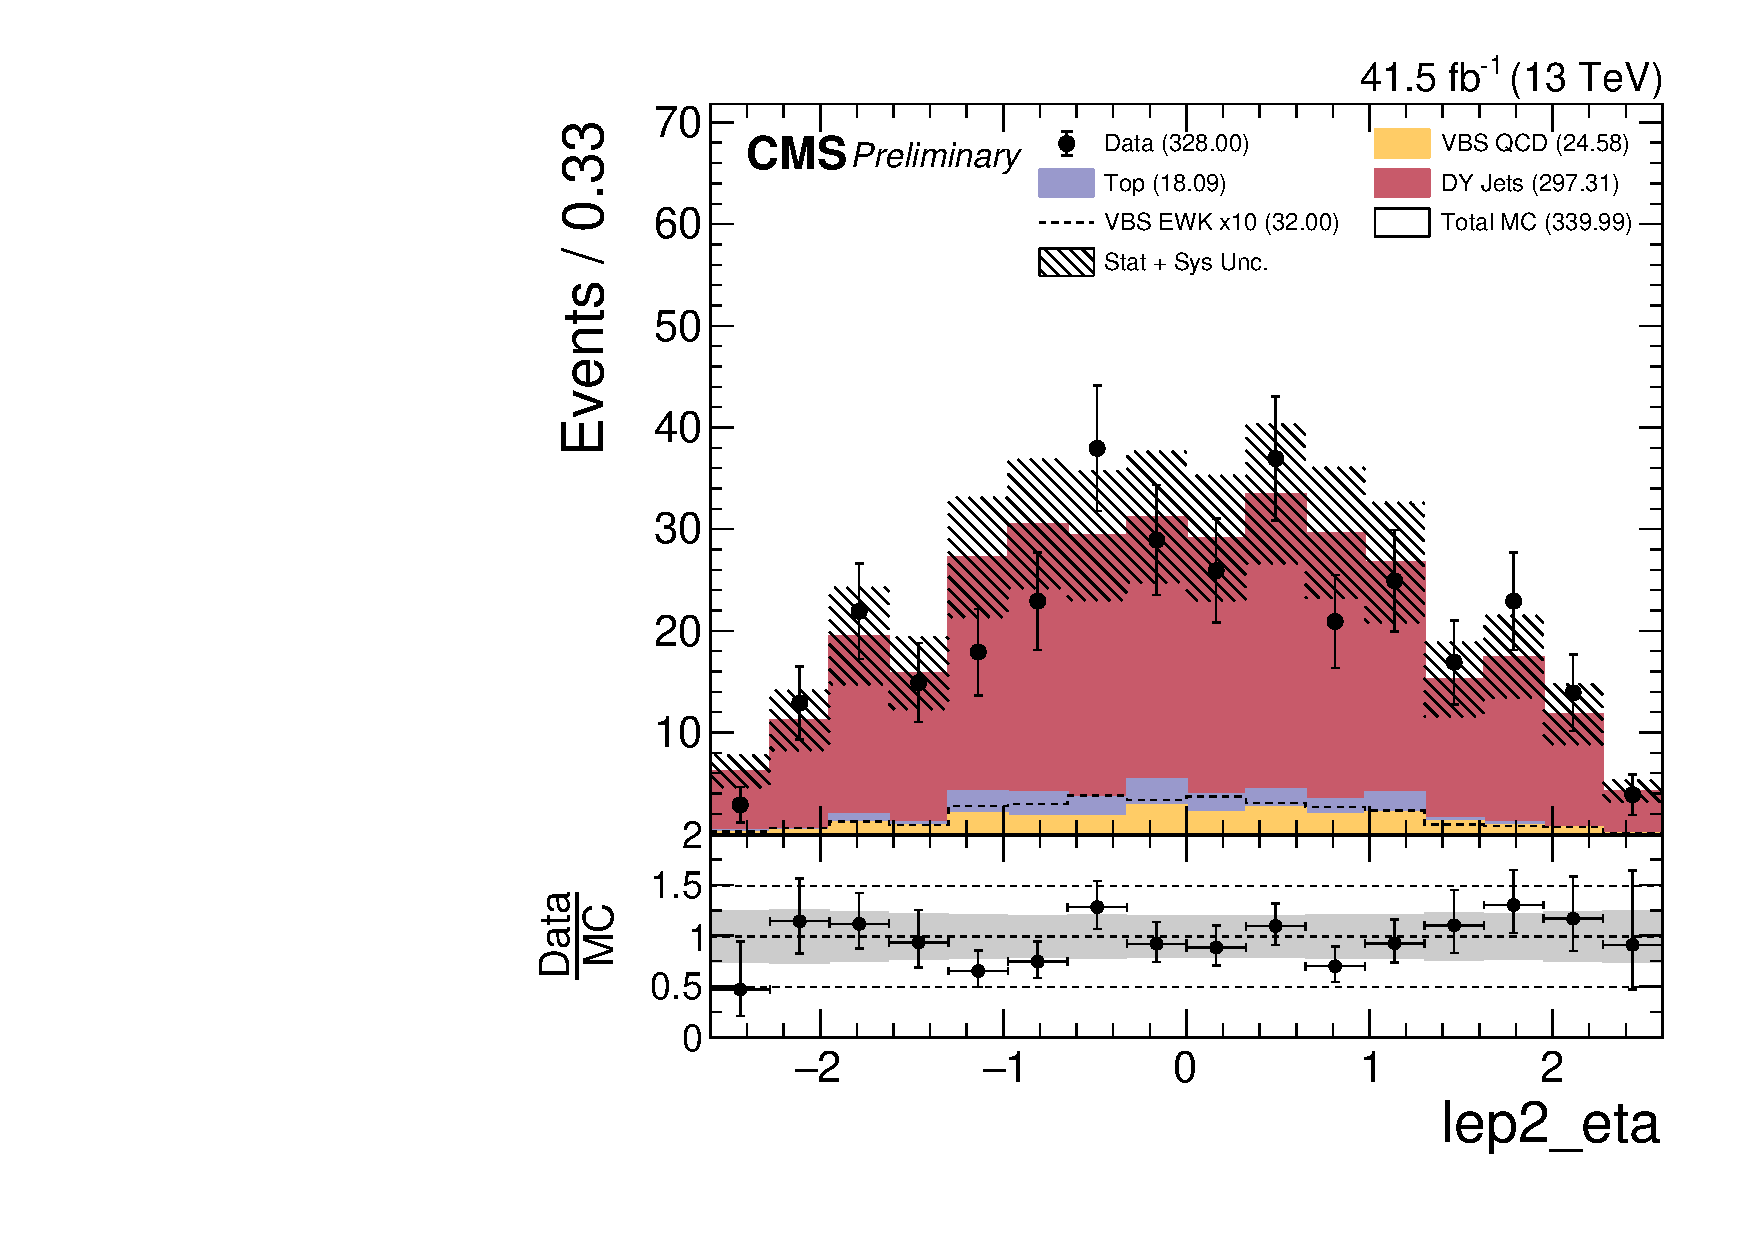
\includegraphics[width=0.30\textwidth]{analysis_plots/2017_zv/cr_vjets_e/lep2_eta.pdf}
  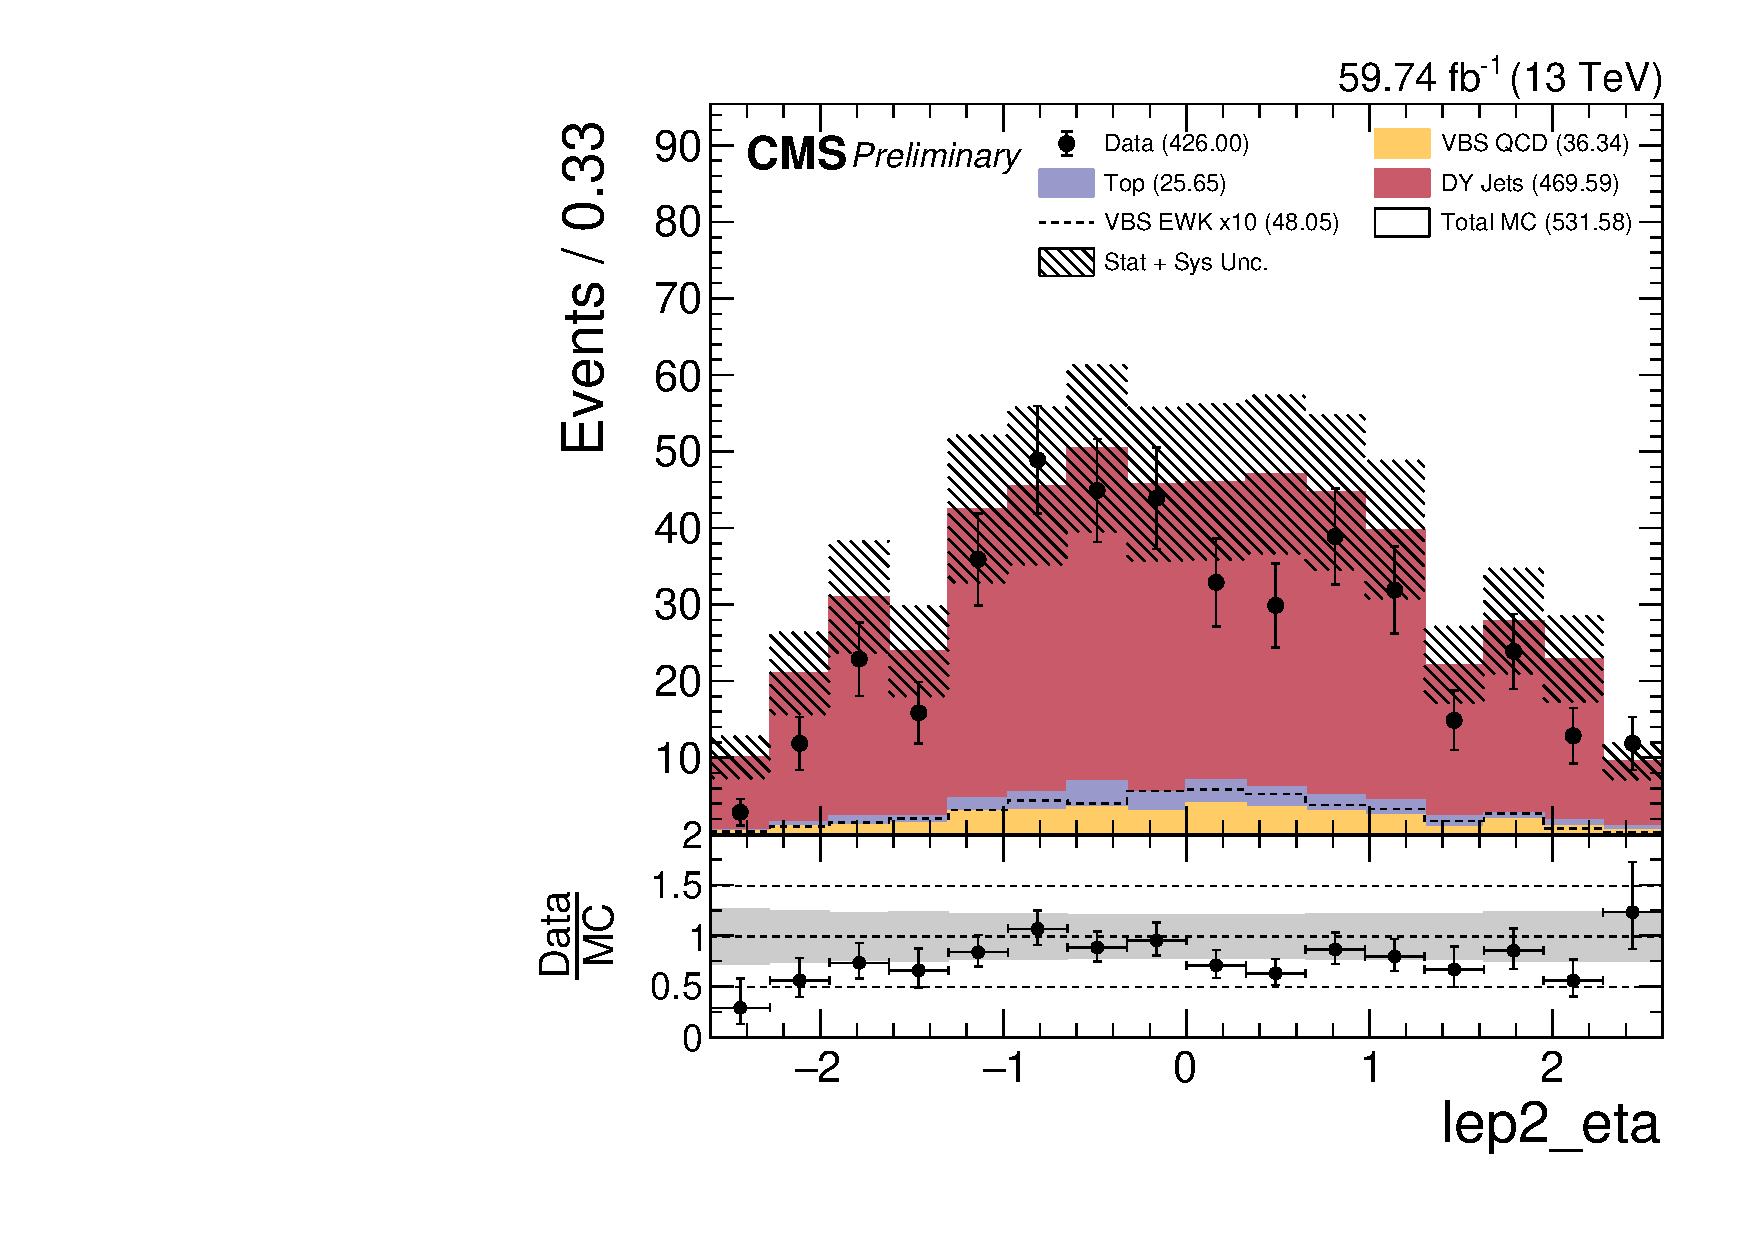
\includegraphics[width=0.30\textwidth]{analysis_plots/2018_zv/cr_vjets_e/lep2_eta.pdf} \\
  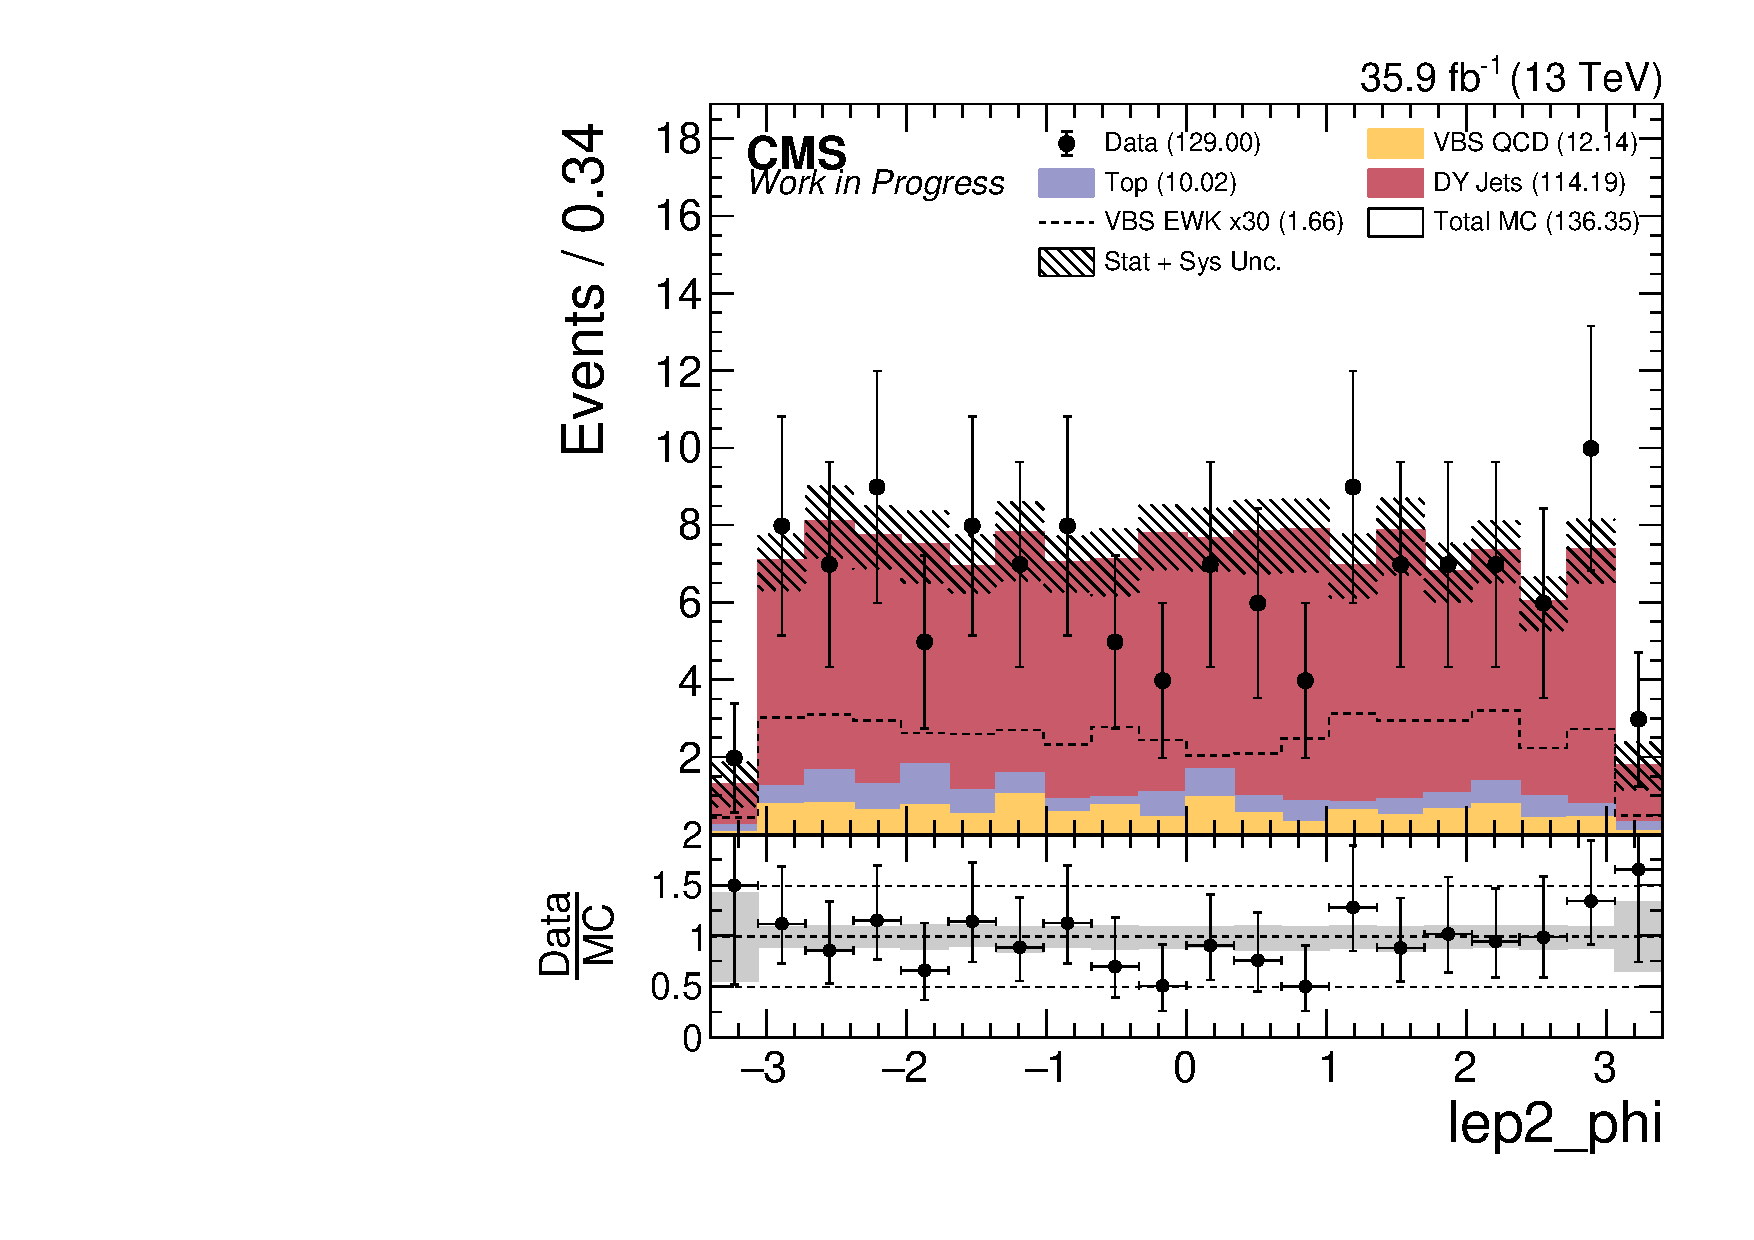
\includegraphics[width=0.30\textwidth]{analysis_plots/2016_zv/cr_vjets_e/lep2_phi.pdf}
  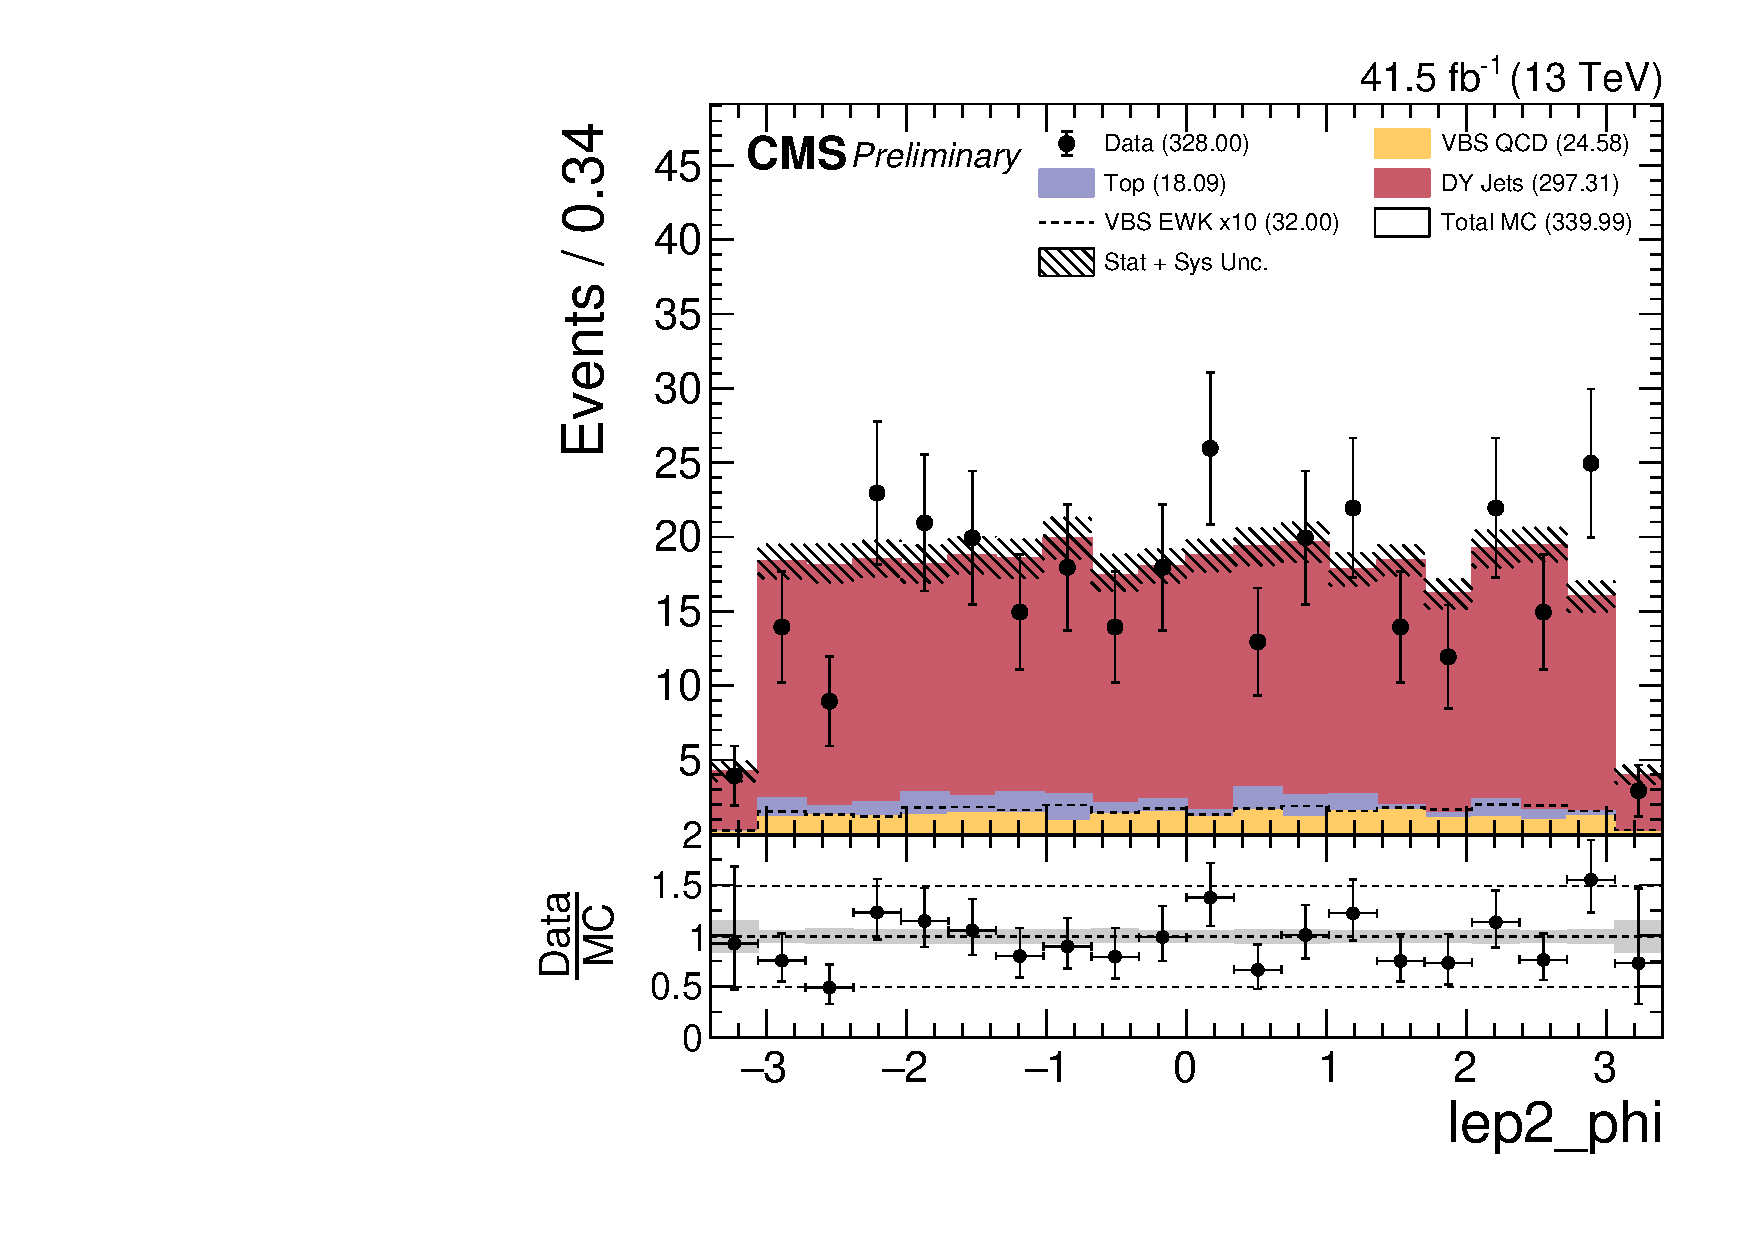
\includegraphics[width=0.30\textwidth]{analysis_plots/2017_zv/cr_vjets_e/lep2_phi.pdf}
  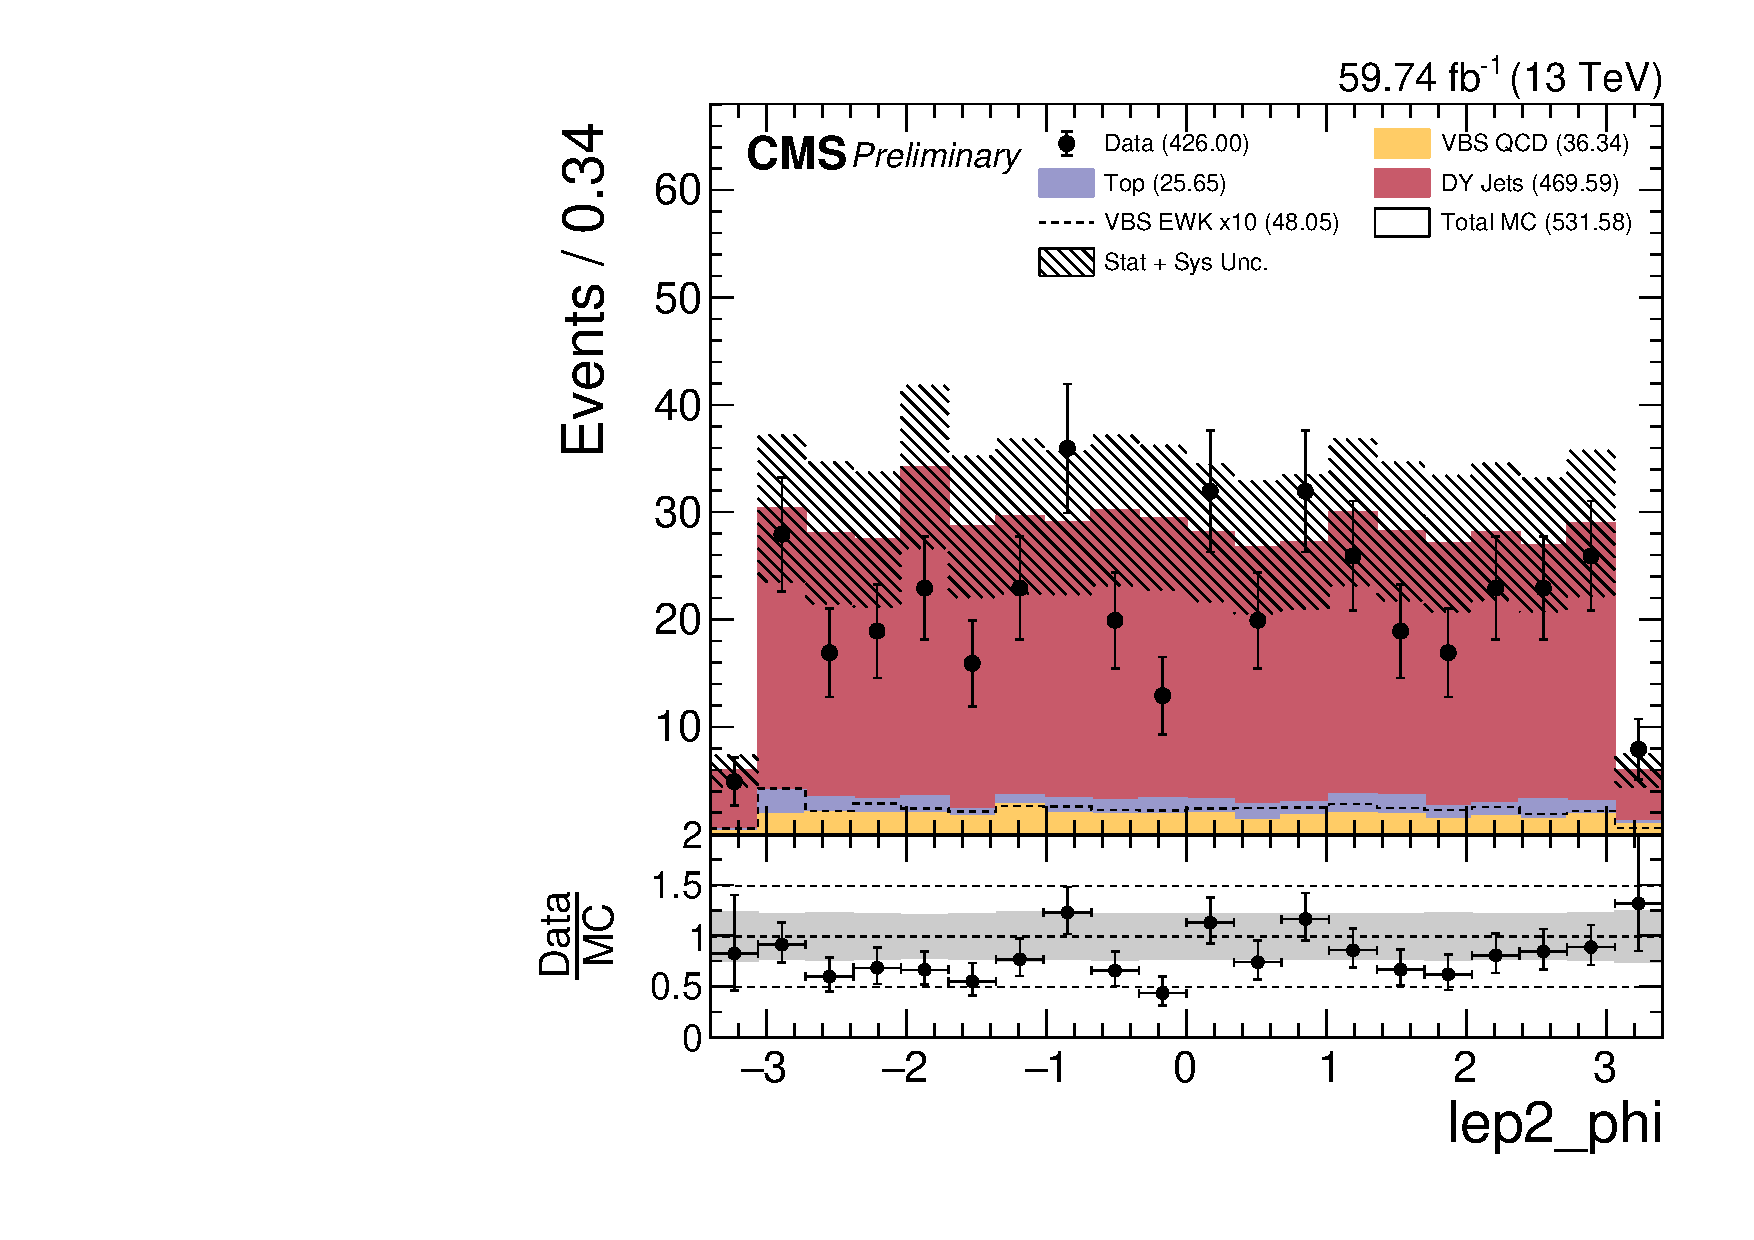
\includegraphics[width=0.30\textwidth]{analysis_plots/2018_zv/cr_vjets_e/lep2_phi.pdf} \\
  \caption[DY+Jets Control Region: Trailing electron kinematics in Boosted ZV Channel]%
  {DY+Jets Control Region: Trailing electron kinematics in Boosted ZV Channel. From Left to Right: 2016,
    2017, and 2018. From Top to Bottom: \( p_T \), \( \eta \), \( \phi \).}%
  \label{fig:zv-cr-vjets-e-lep2-pt-eta-phi}
\end{figure}

\begin{figure}[!ht]
  \centering
  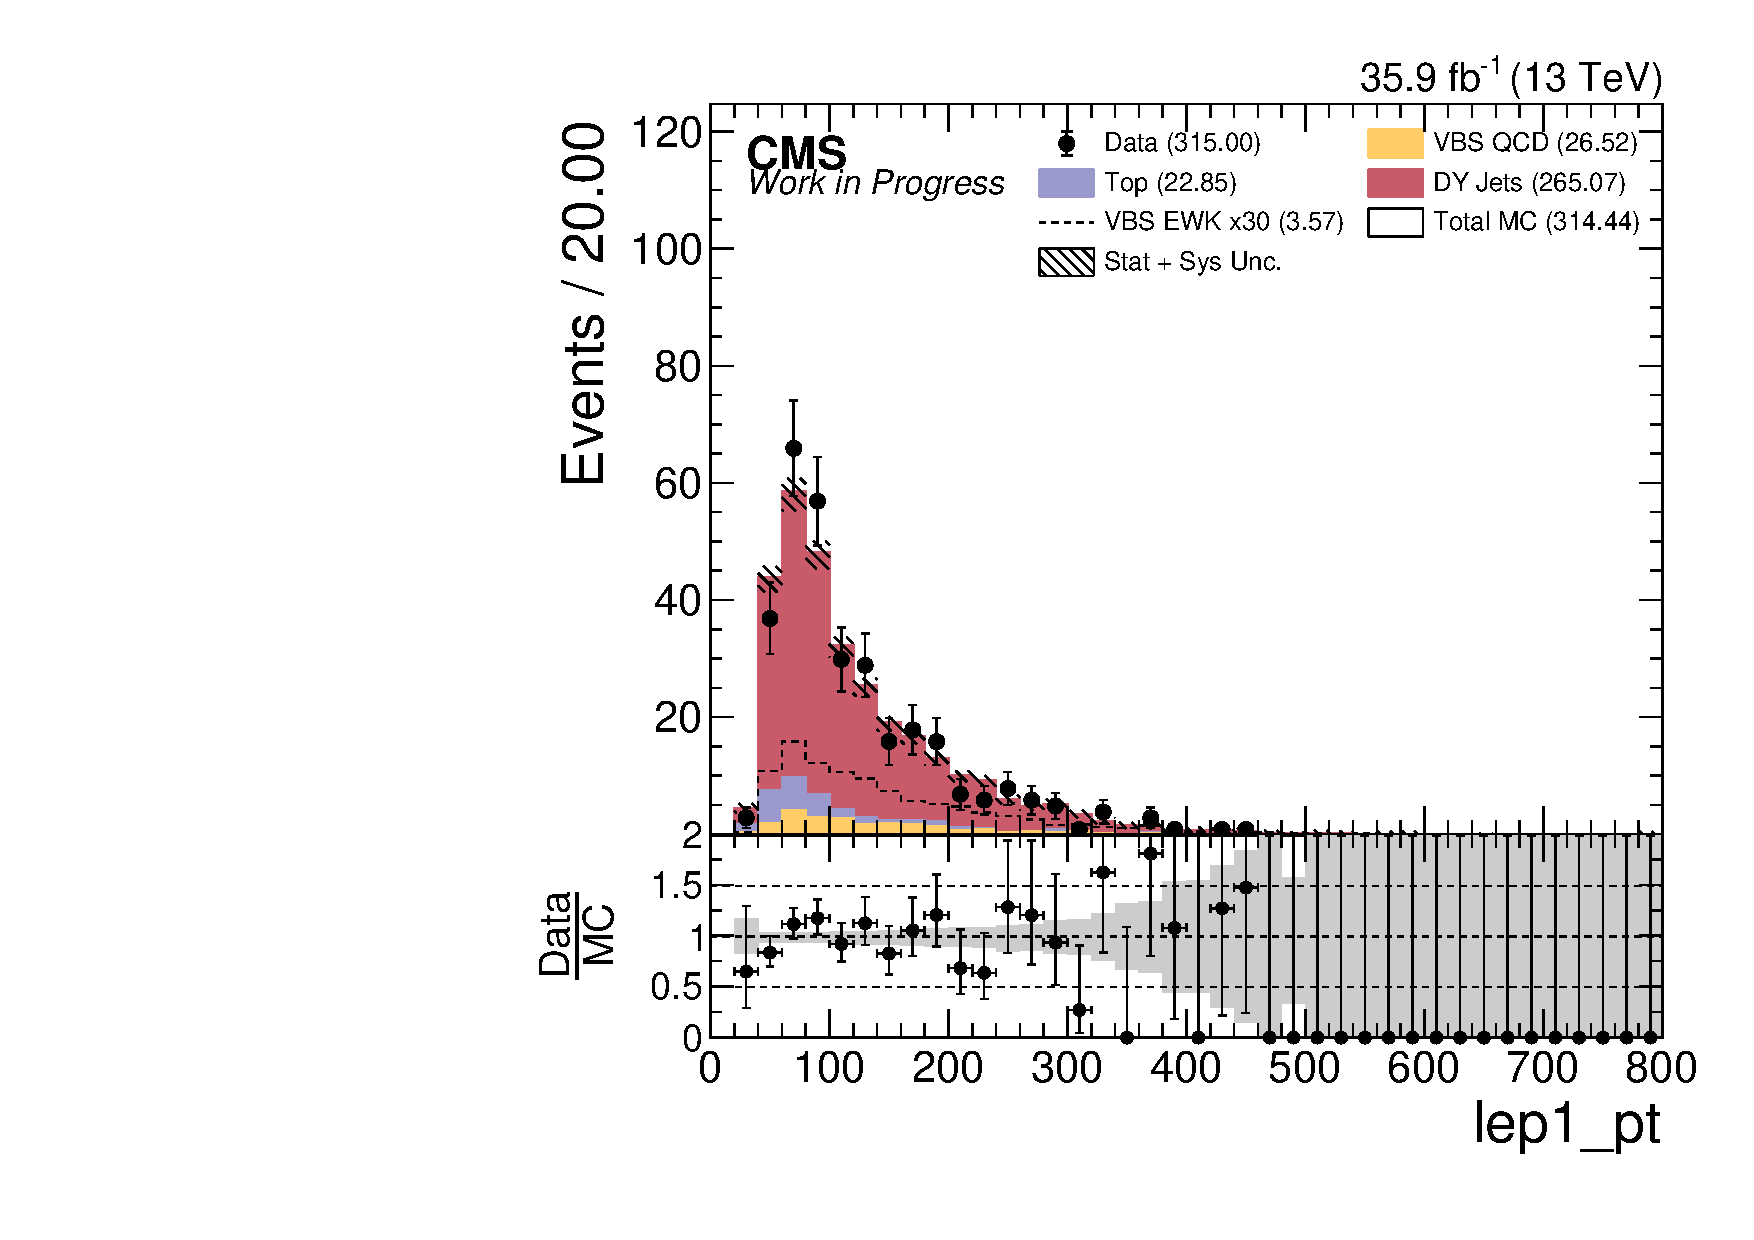
\includegraphics[width=0.30\textwidth]{analysis_plots/2016_zv/cr_vjets_m/lep1_pt.pdf}
  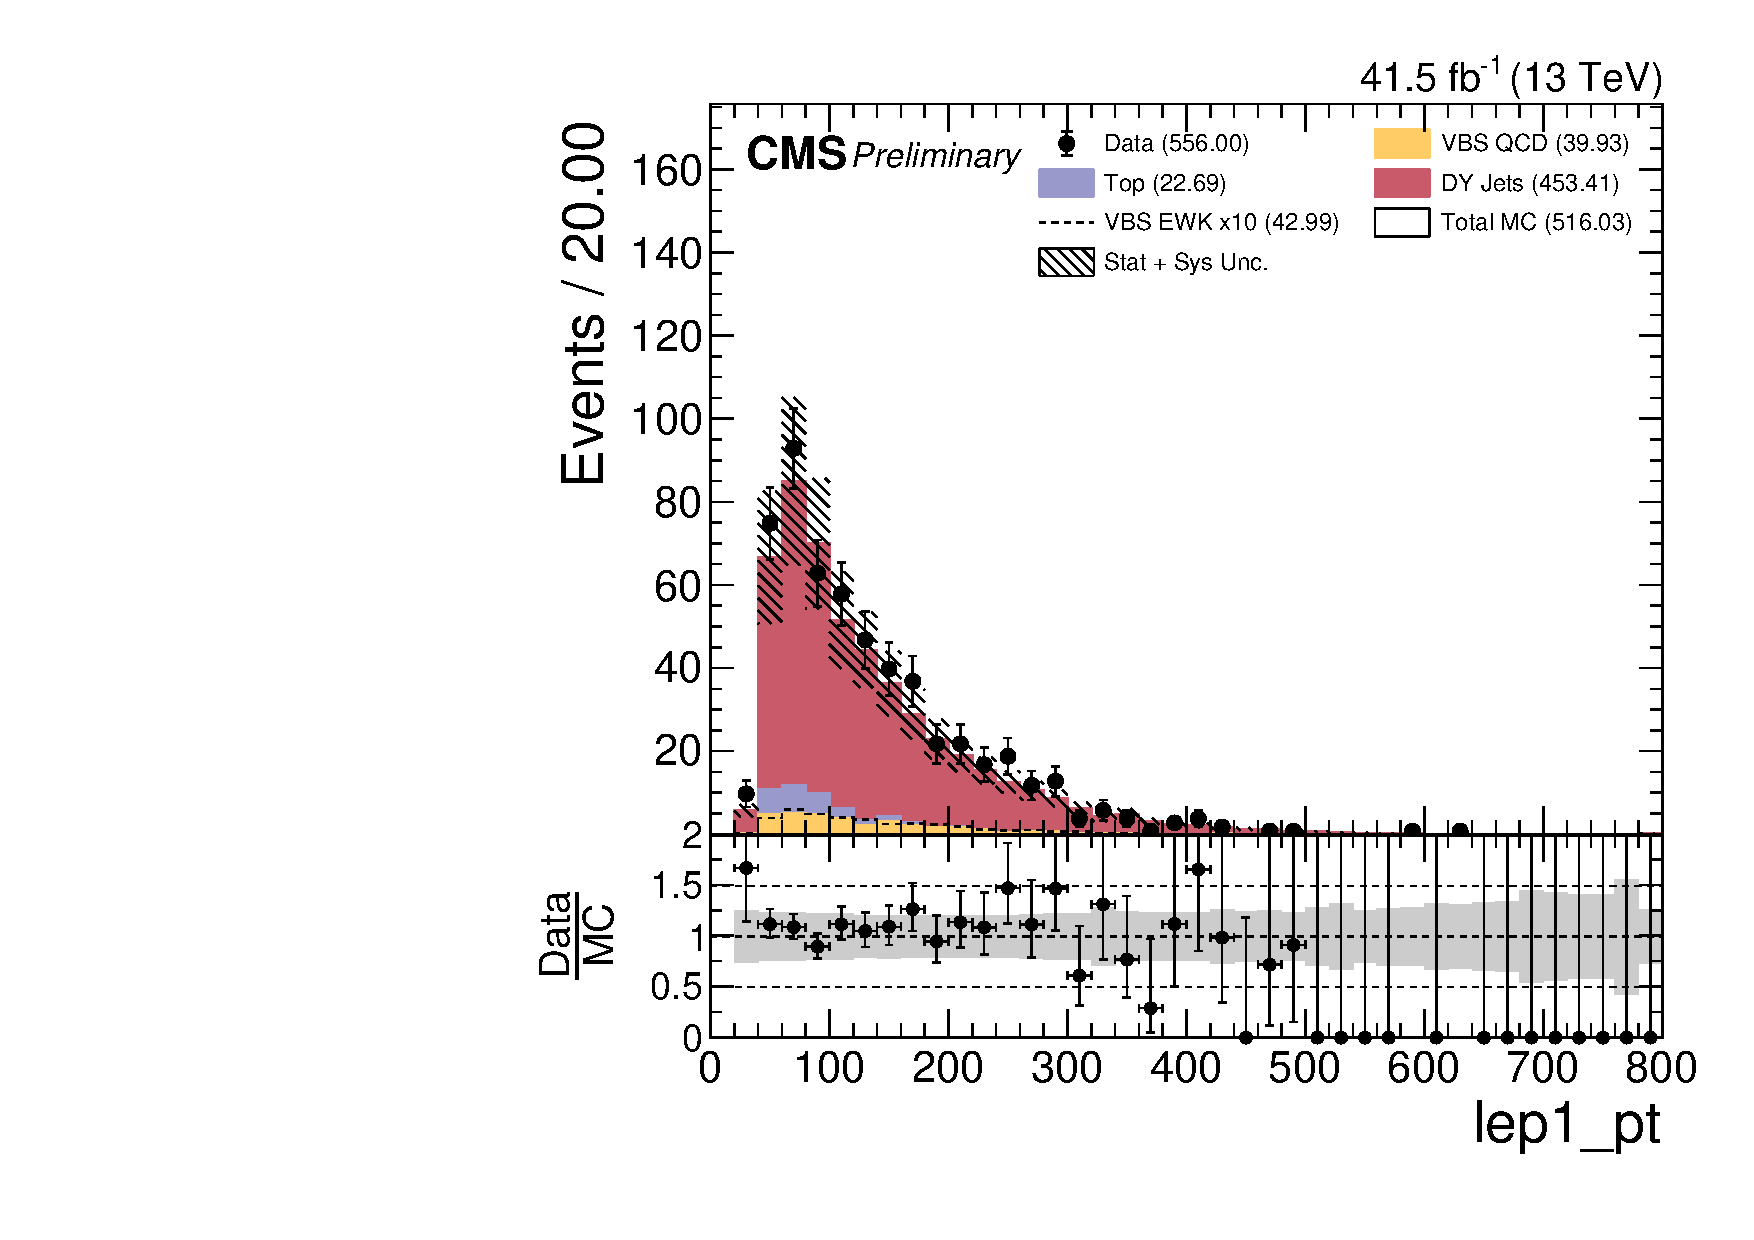
\includegraphics[width=0.30\textwidth]{analysis_plots/2017_zv/cr_vjets_m/lep1_pt.pdf}
  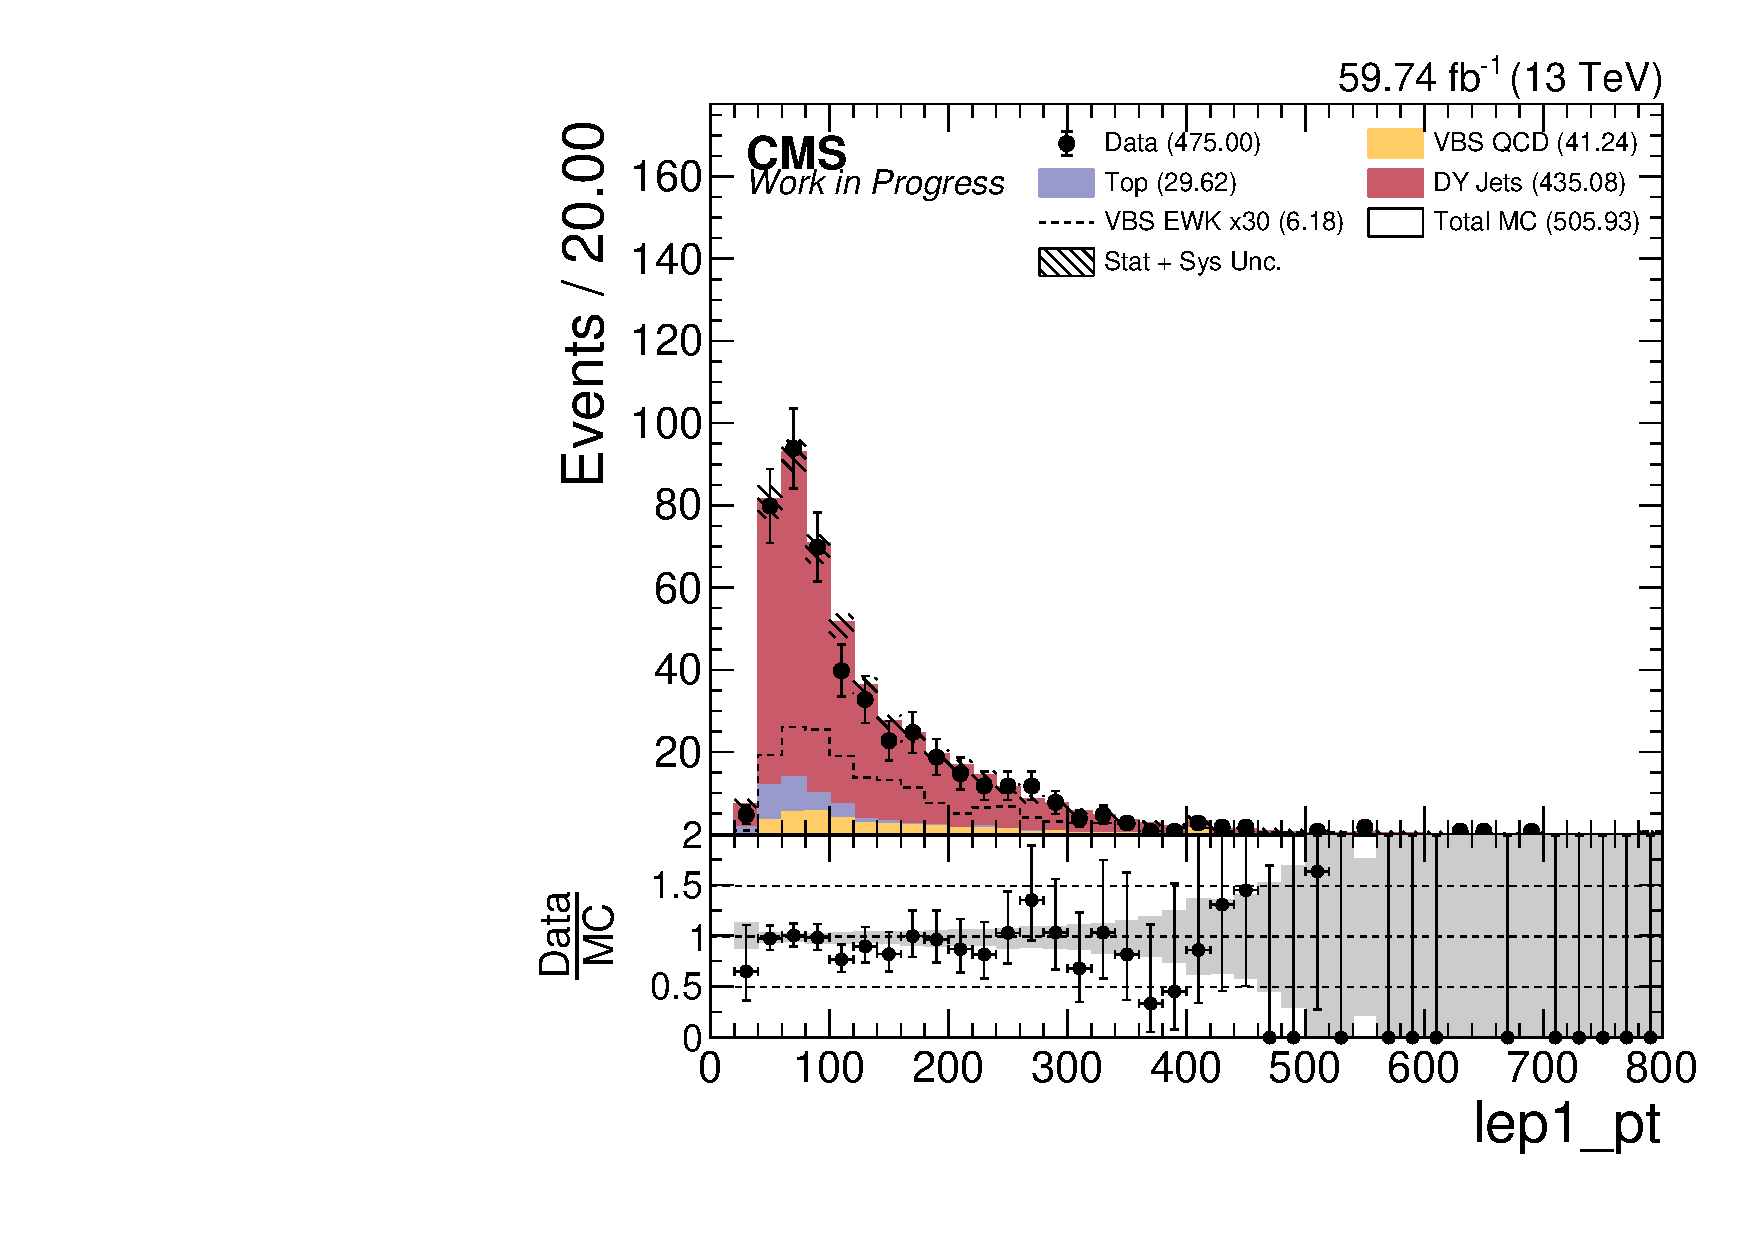
\includegraphics[width=0.30\textwidth]{analysis_plots/2018_zv/cr_vjets_m/lep1_pt.pdf} \\
  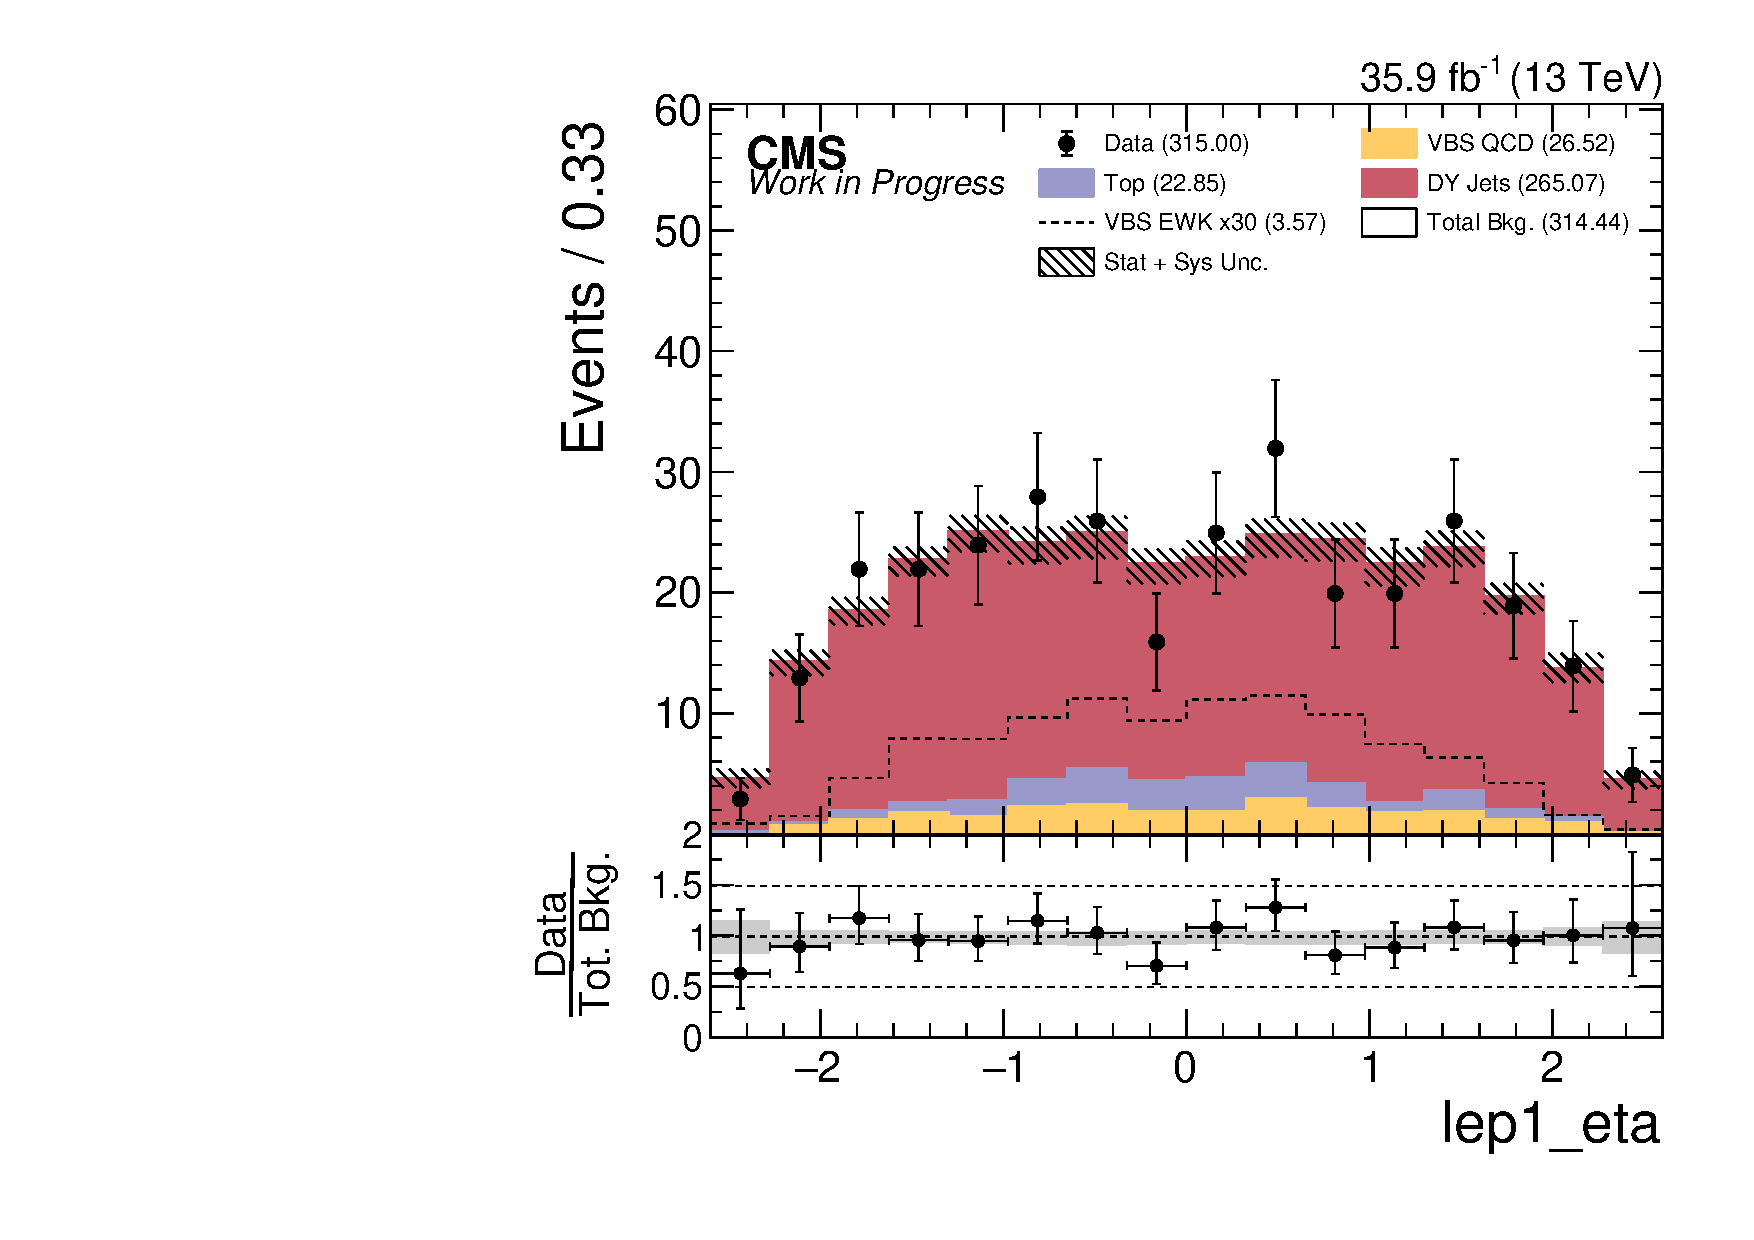
\includegraphics[width=0.30\textwidth]{analysis_plots/2016_zv/cr_vjets_m/lep1_eta.pdf}
  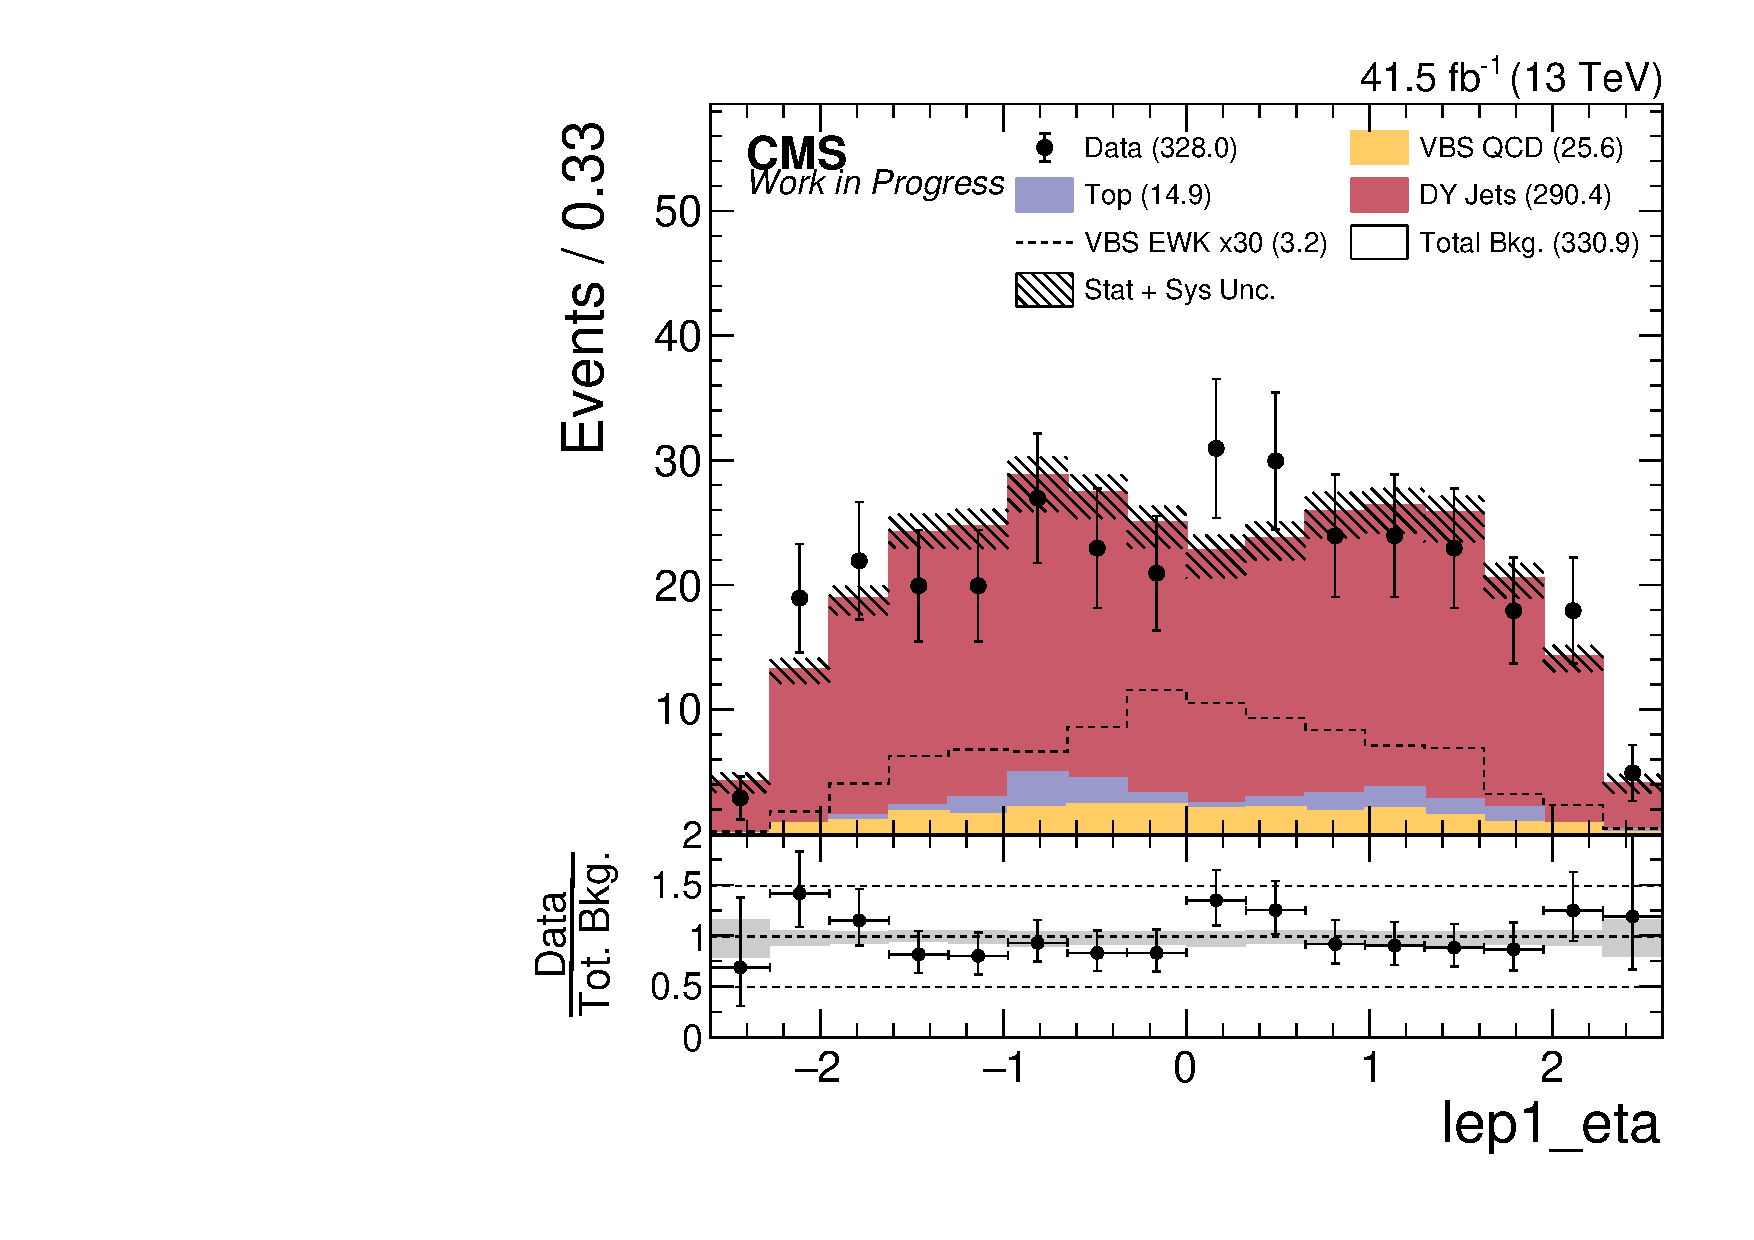
\includegraphics[width=0.30\textwidth]{analysis_plots/2017_zv/cr_vjets_m/lep1_eta.pdf}
  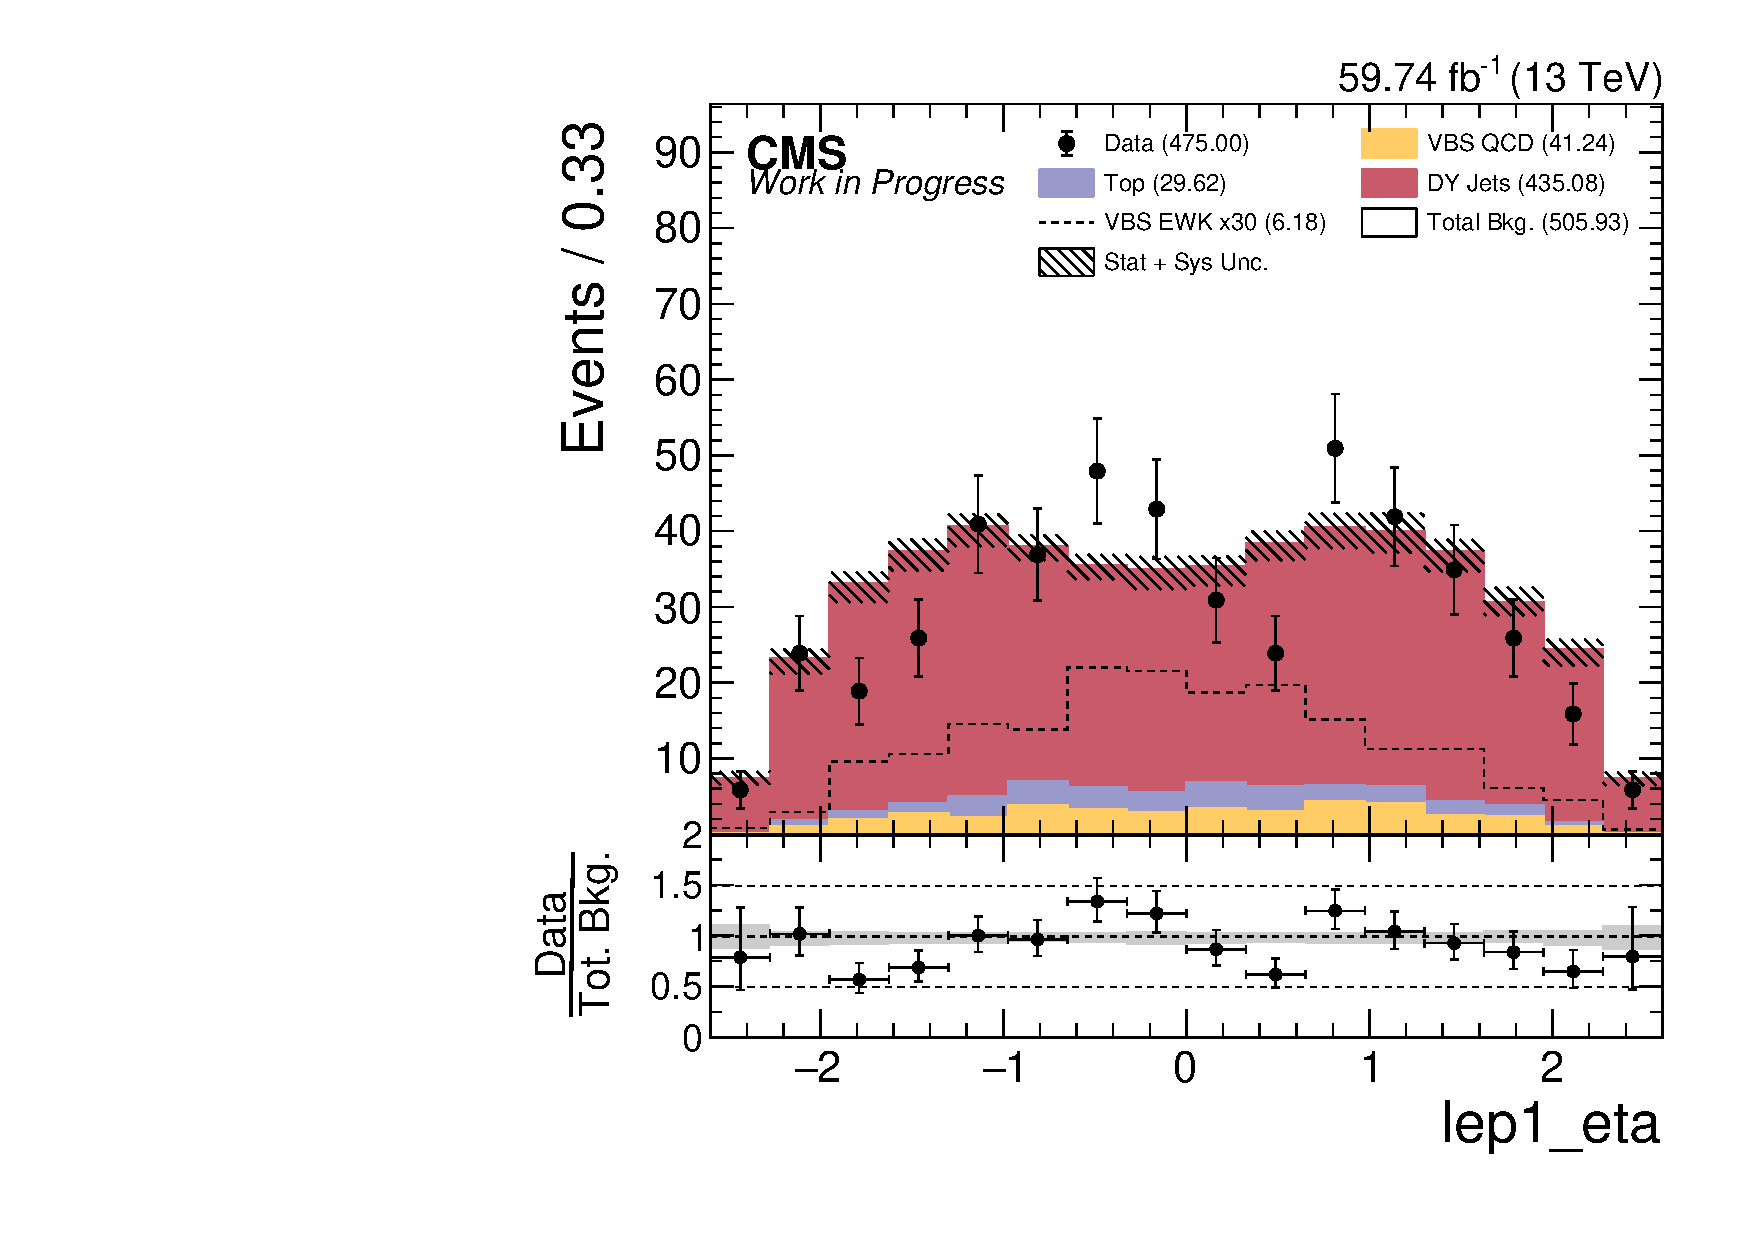
\includegraphics[width=0.30\textwidth]{analysis_plots/2018_zv/cr_vjets_m/lep1_eta.pdf} \\
  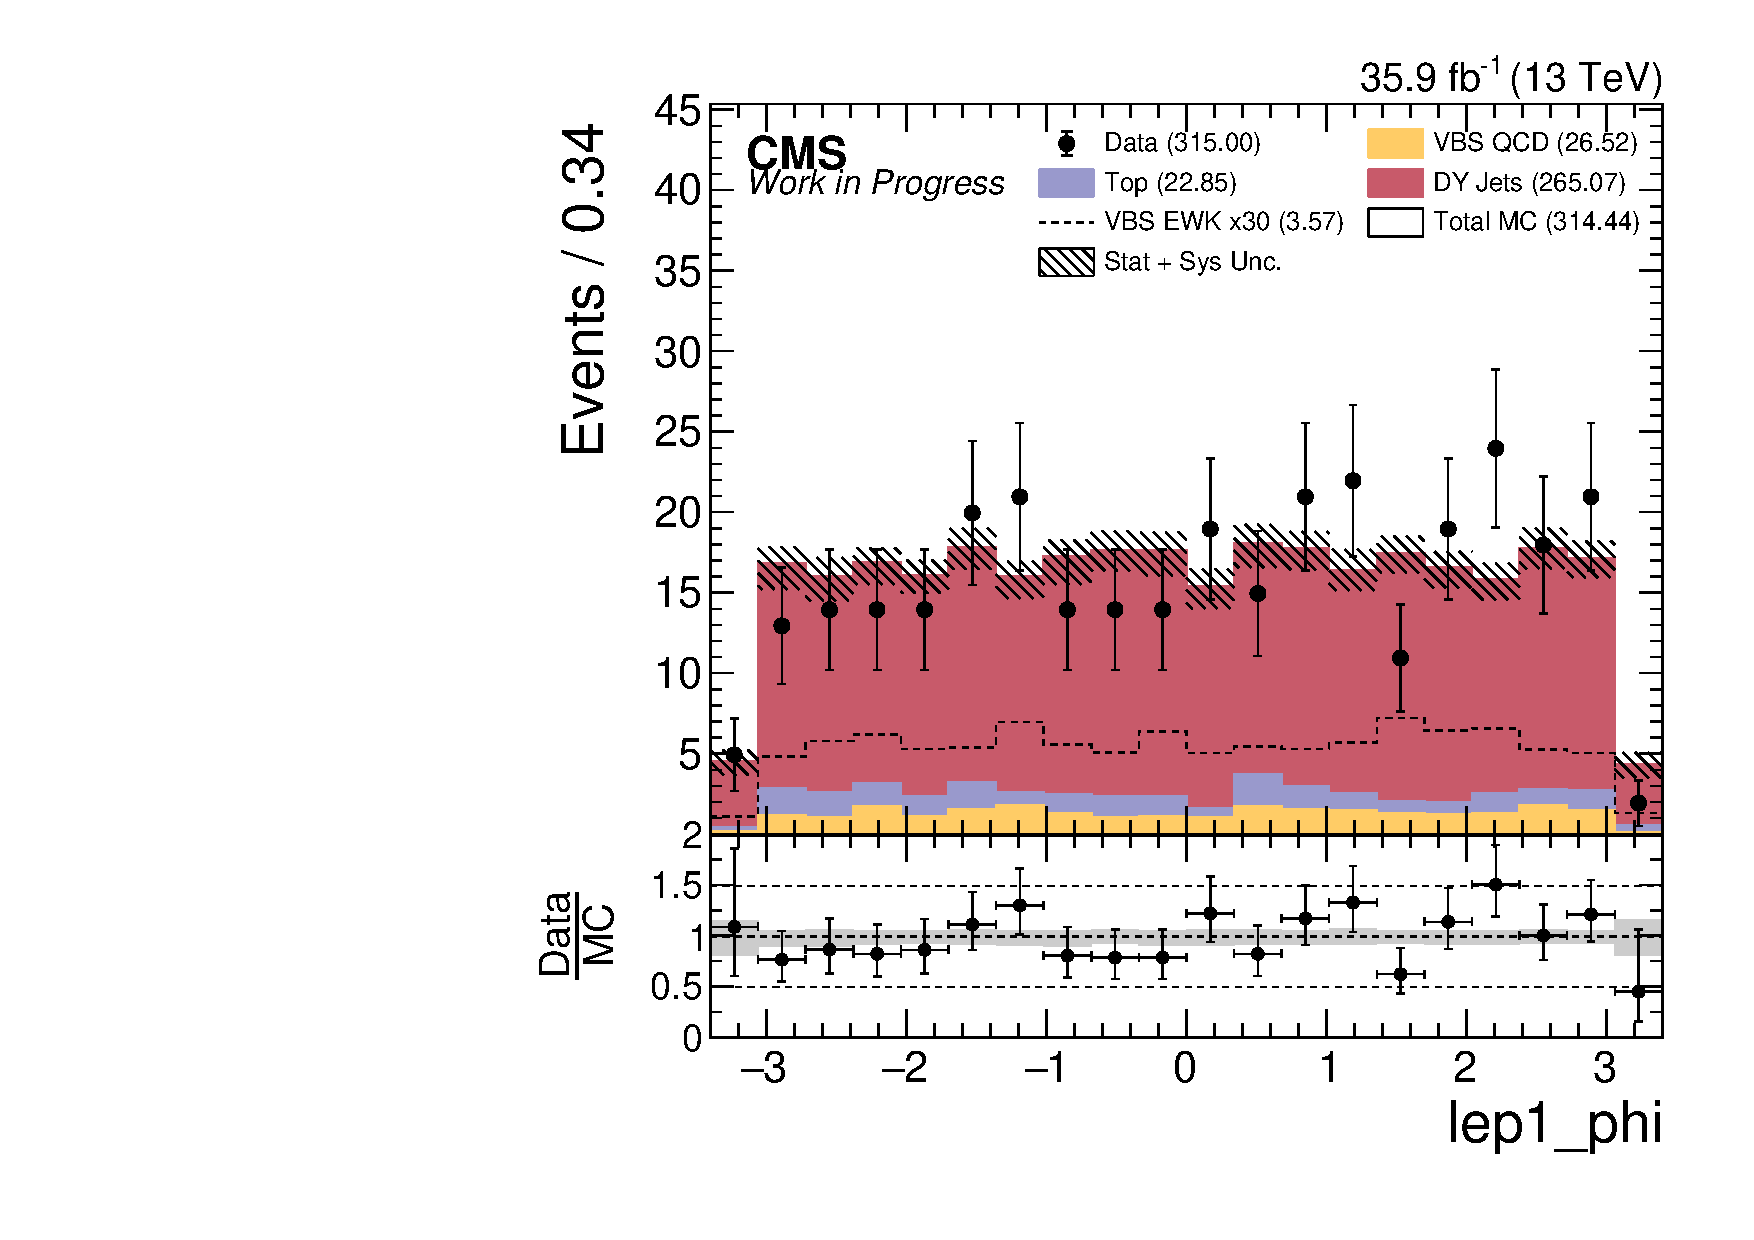
\includegraphics[width=0.30\textwidth]{analysis_plots/2016_zv/cr_vjets_m/lep1_phi.pdf}
  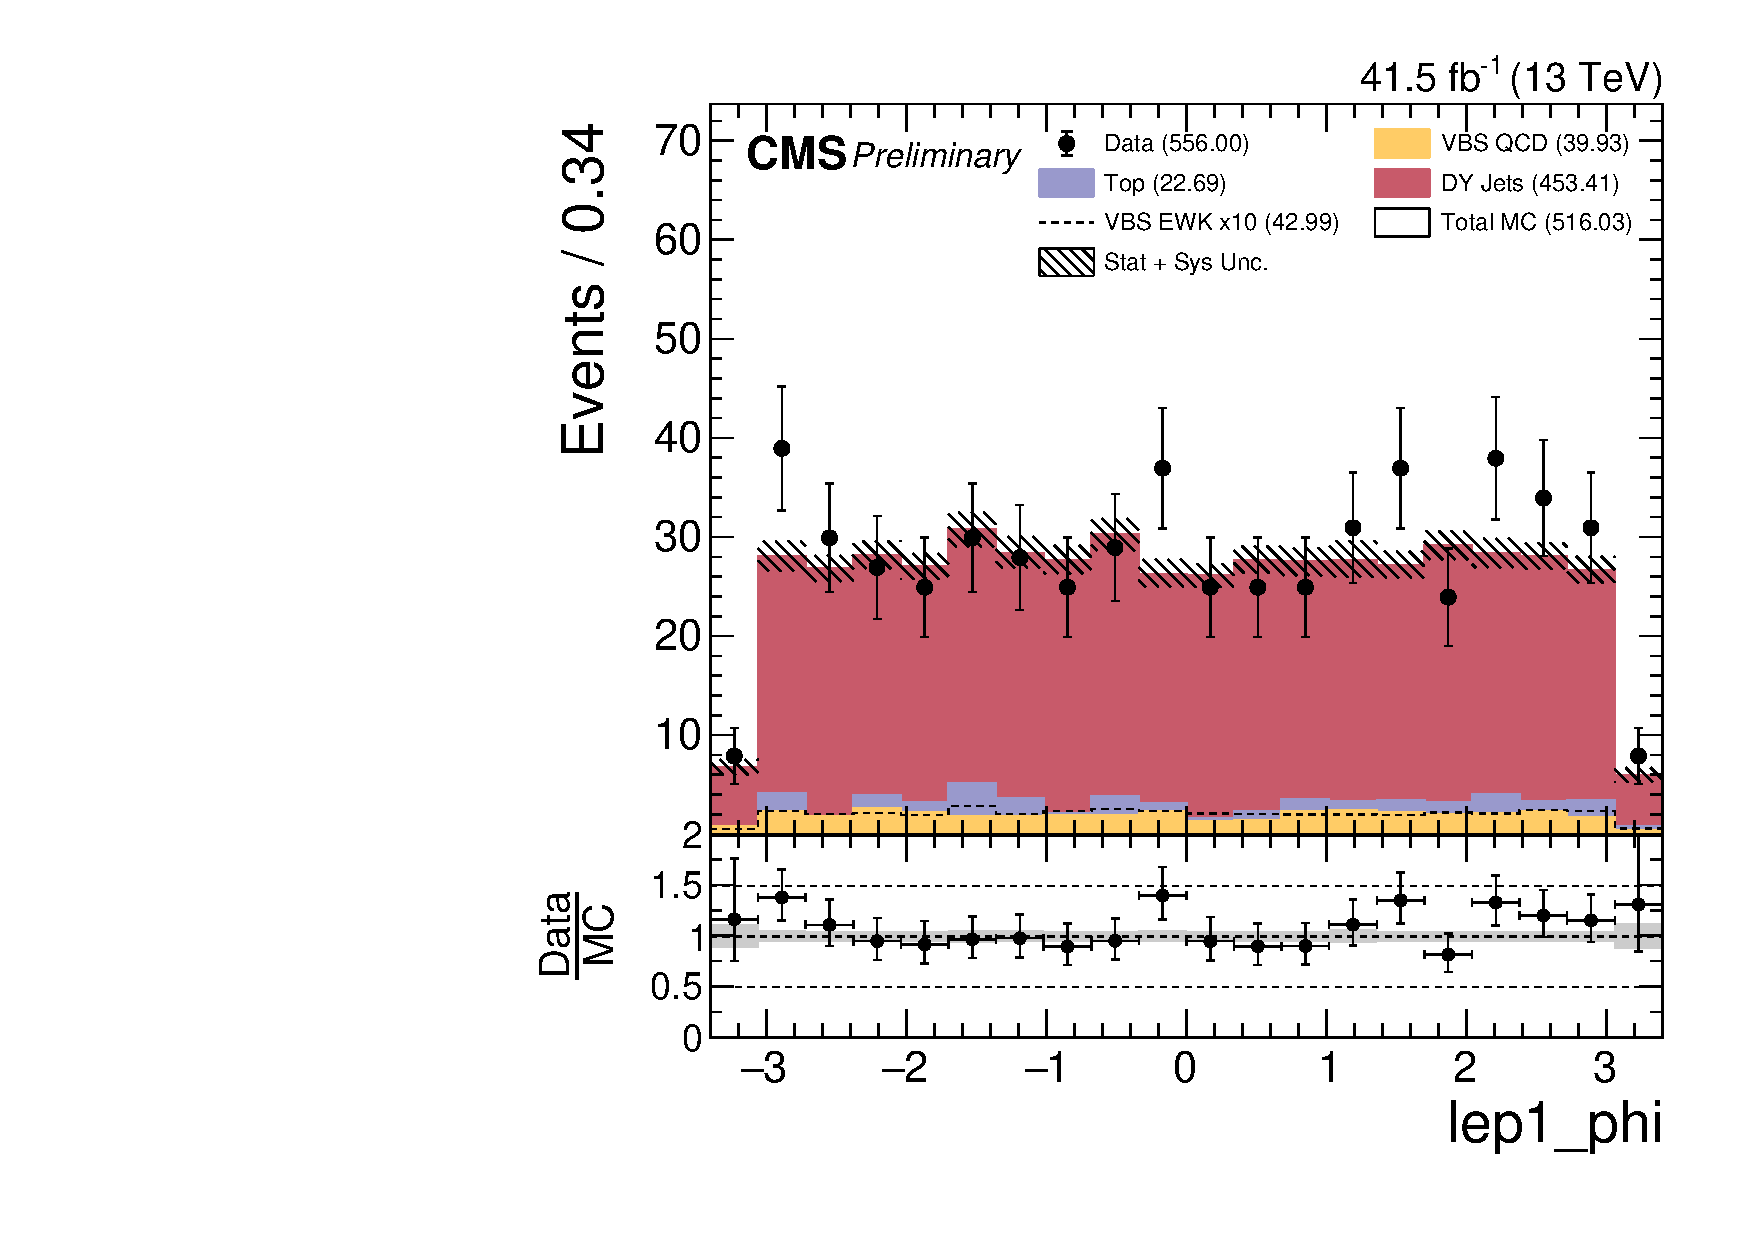
\includegraphics[width=0.30\textwidth]{analysis_plots/2017_zv/cr_vjets_m/lep1_phi.pdf}
  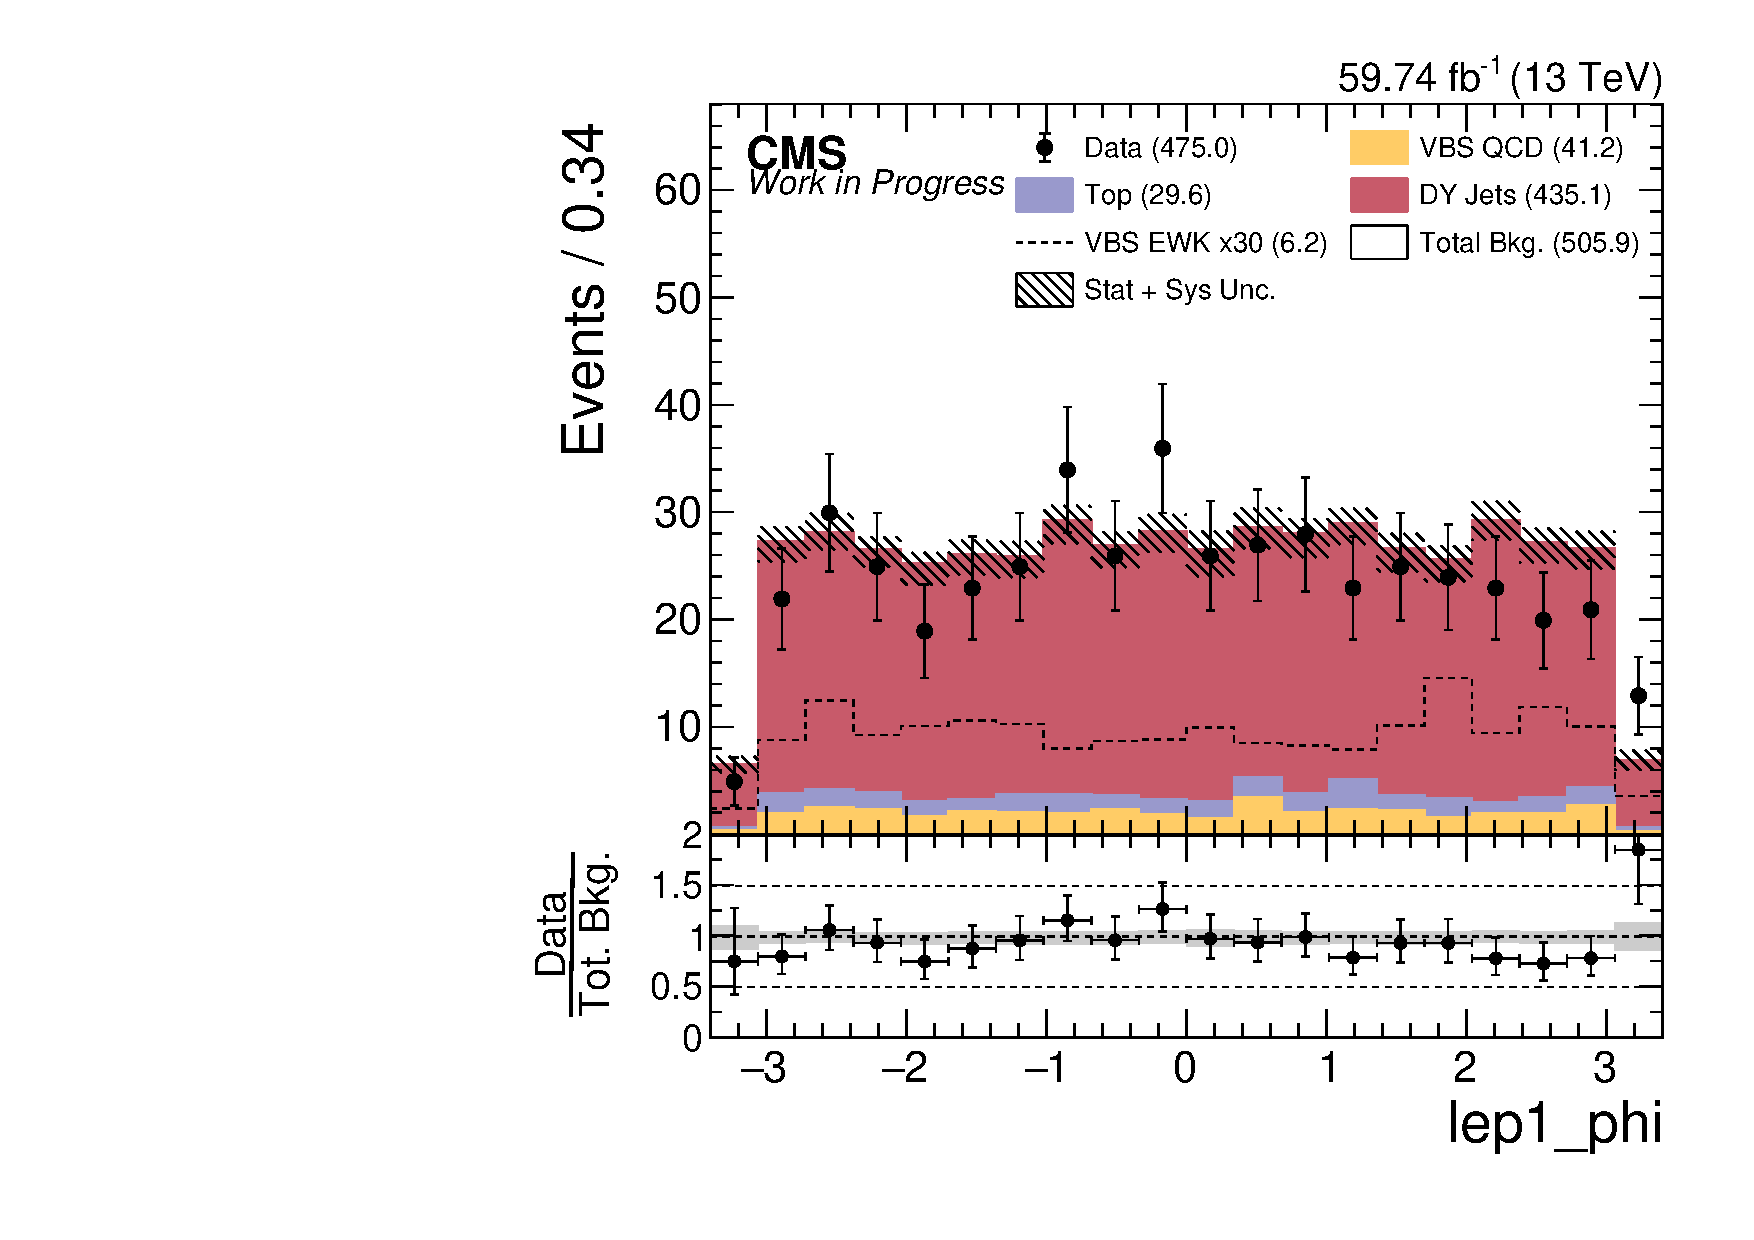
\includegraphics[width=0.30\textwidth]{analysis_plots/2018_zv/cr_vjets_m/lep1_phi.pdf} \\
  \caption[DY+Jets Control Region: Leading muon kinematics in Boosted ZV Channel]%
  {DY+Jets Control Region: Leading muon kinematics in Boosted ZV Channel. From Left to Right: 2016,
    2017, and 2018. From Top to Bottom: \( p_T \), \( \eta \), \( \phi \).}%
  \label{fig:zv-cr-vjets-m-lep1-pt-eta-phi}
\end{figure}

\begin{figure}[!ht]
  \centering
  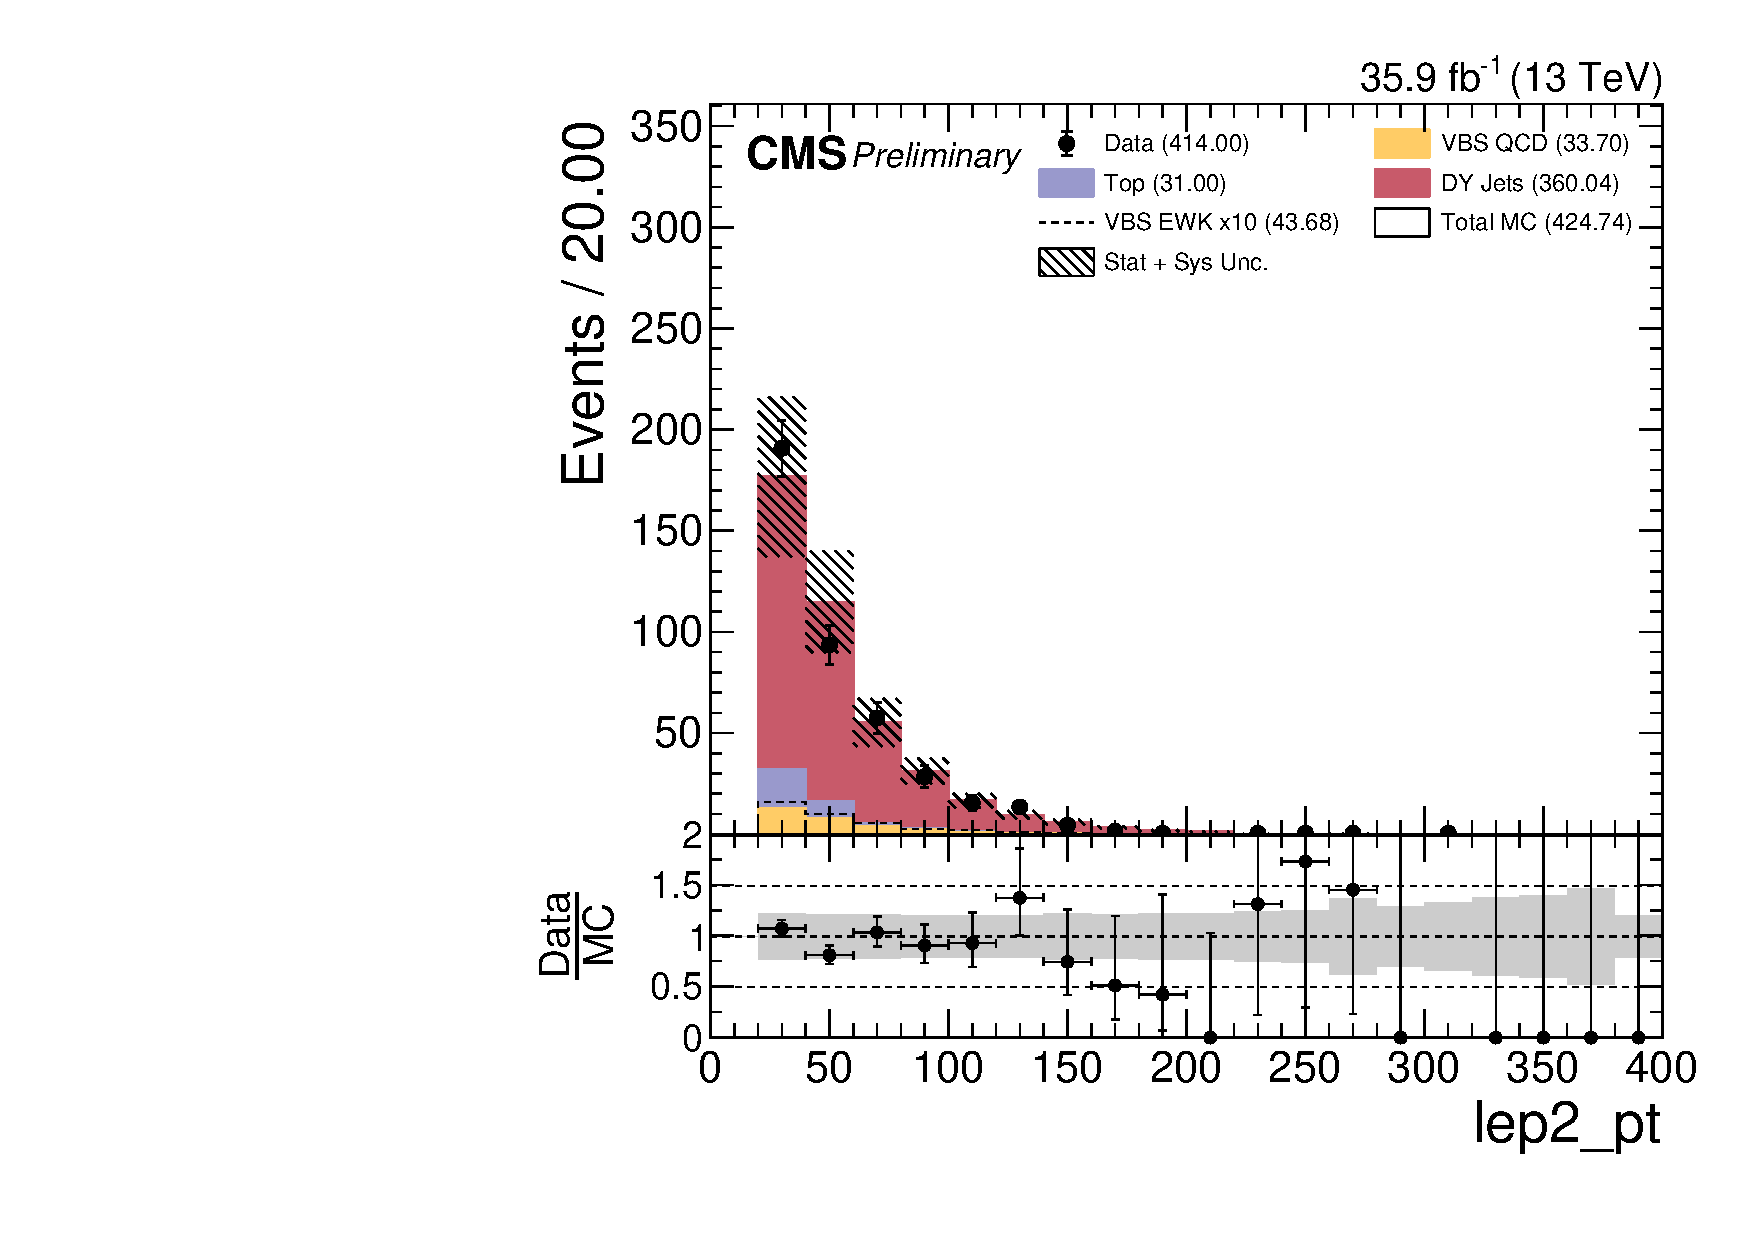
\includegraphics[width=0.30\textwidth]{analysis_plots/2016_zv/cr_vjets_m/lep2_pt.pdf}
  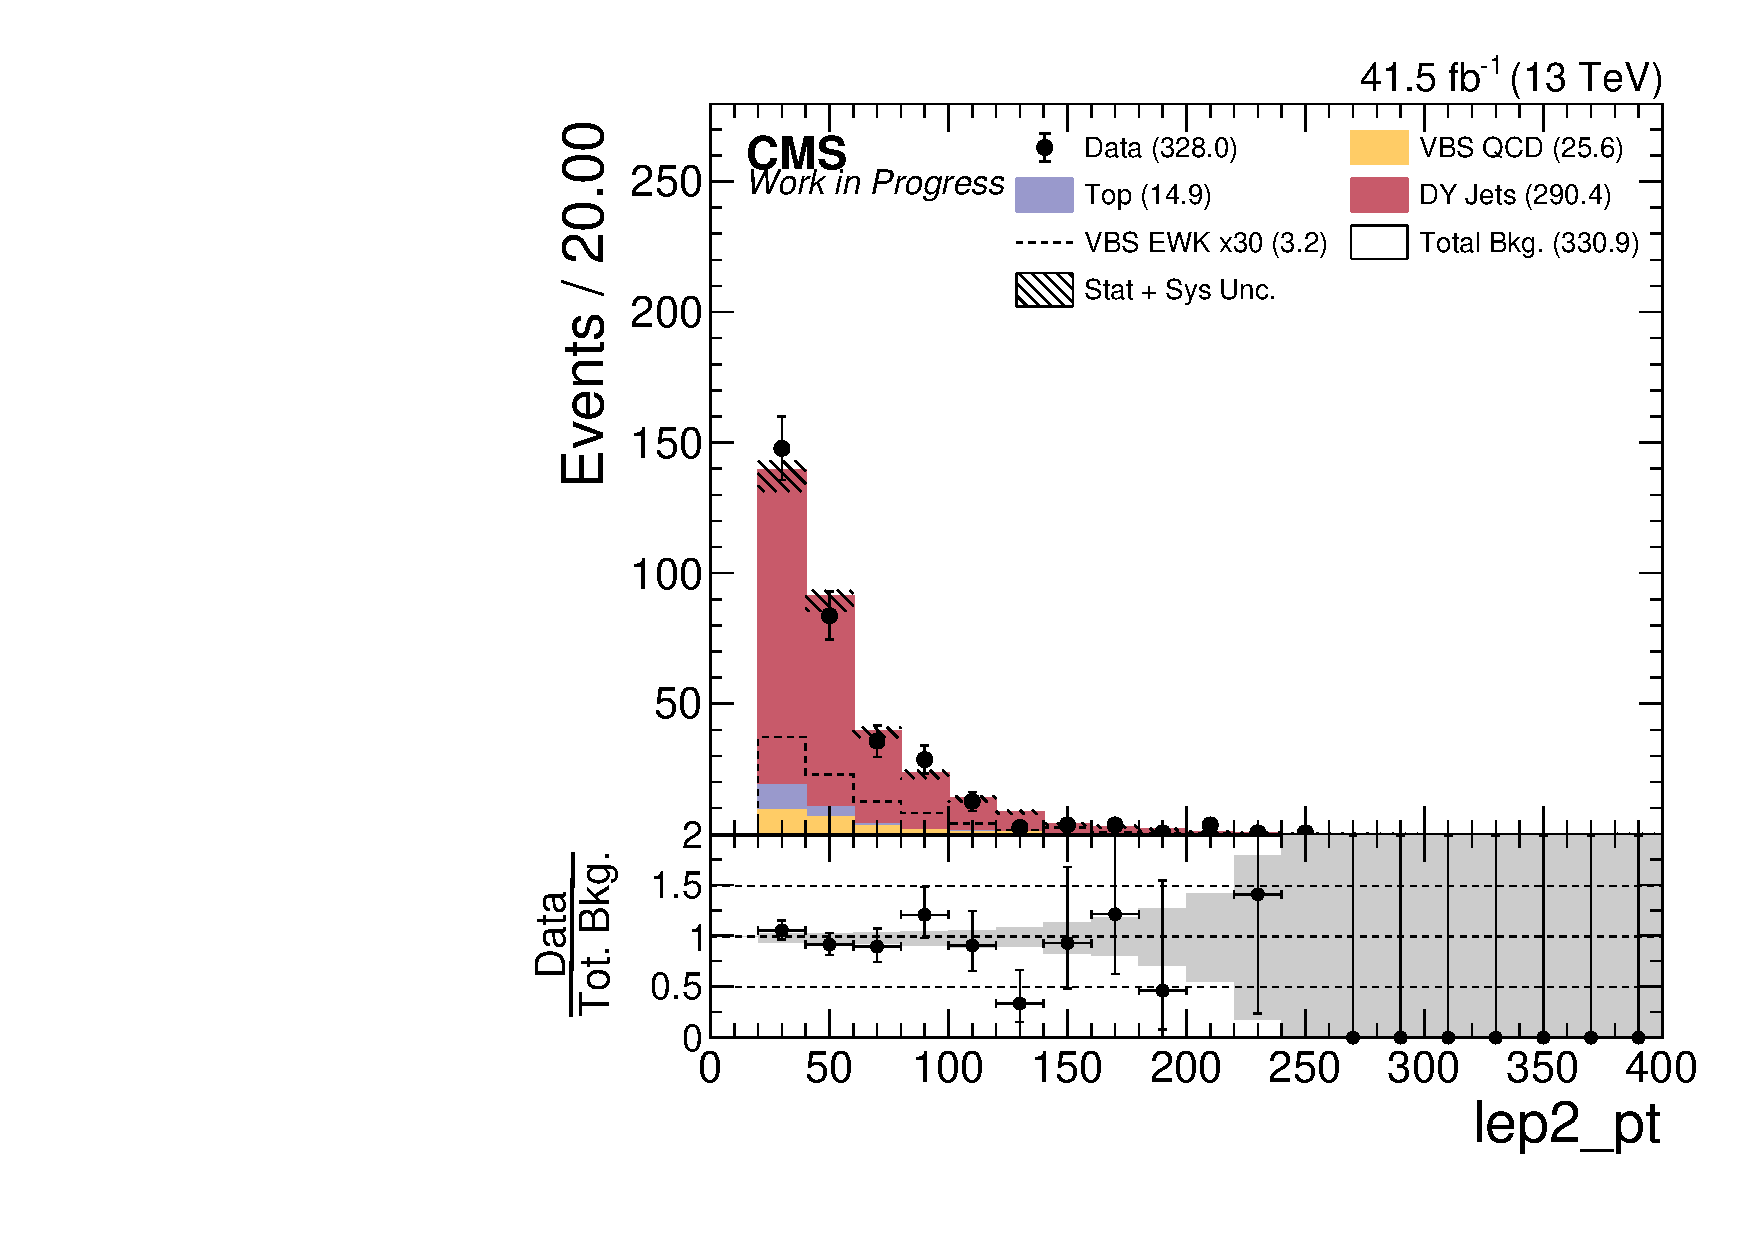
\includegraphics[width=0.30\textwidth]{analysis_plots/2017_zv/cr_vjets_m/lep2_pt.pdf}
  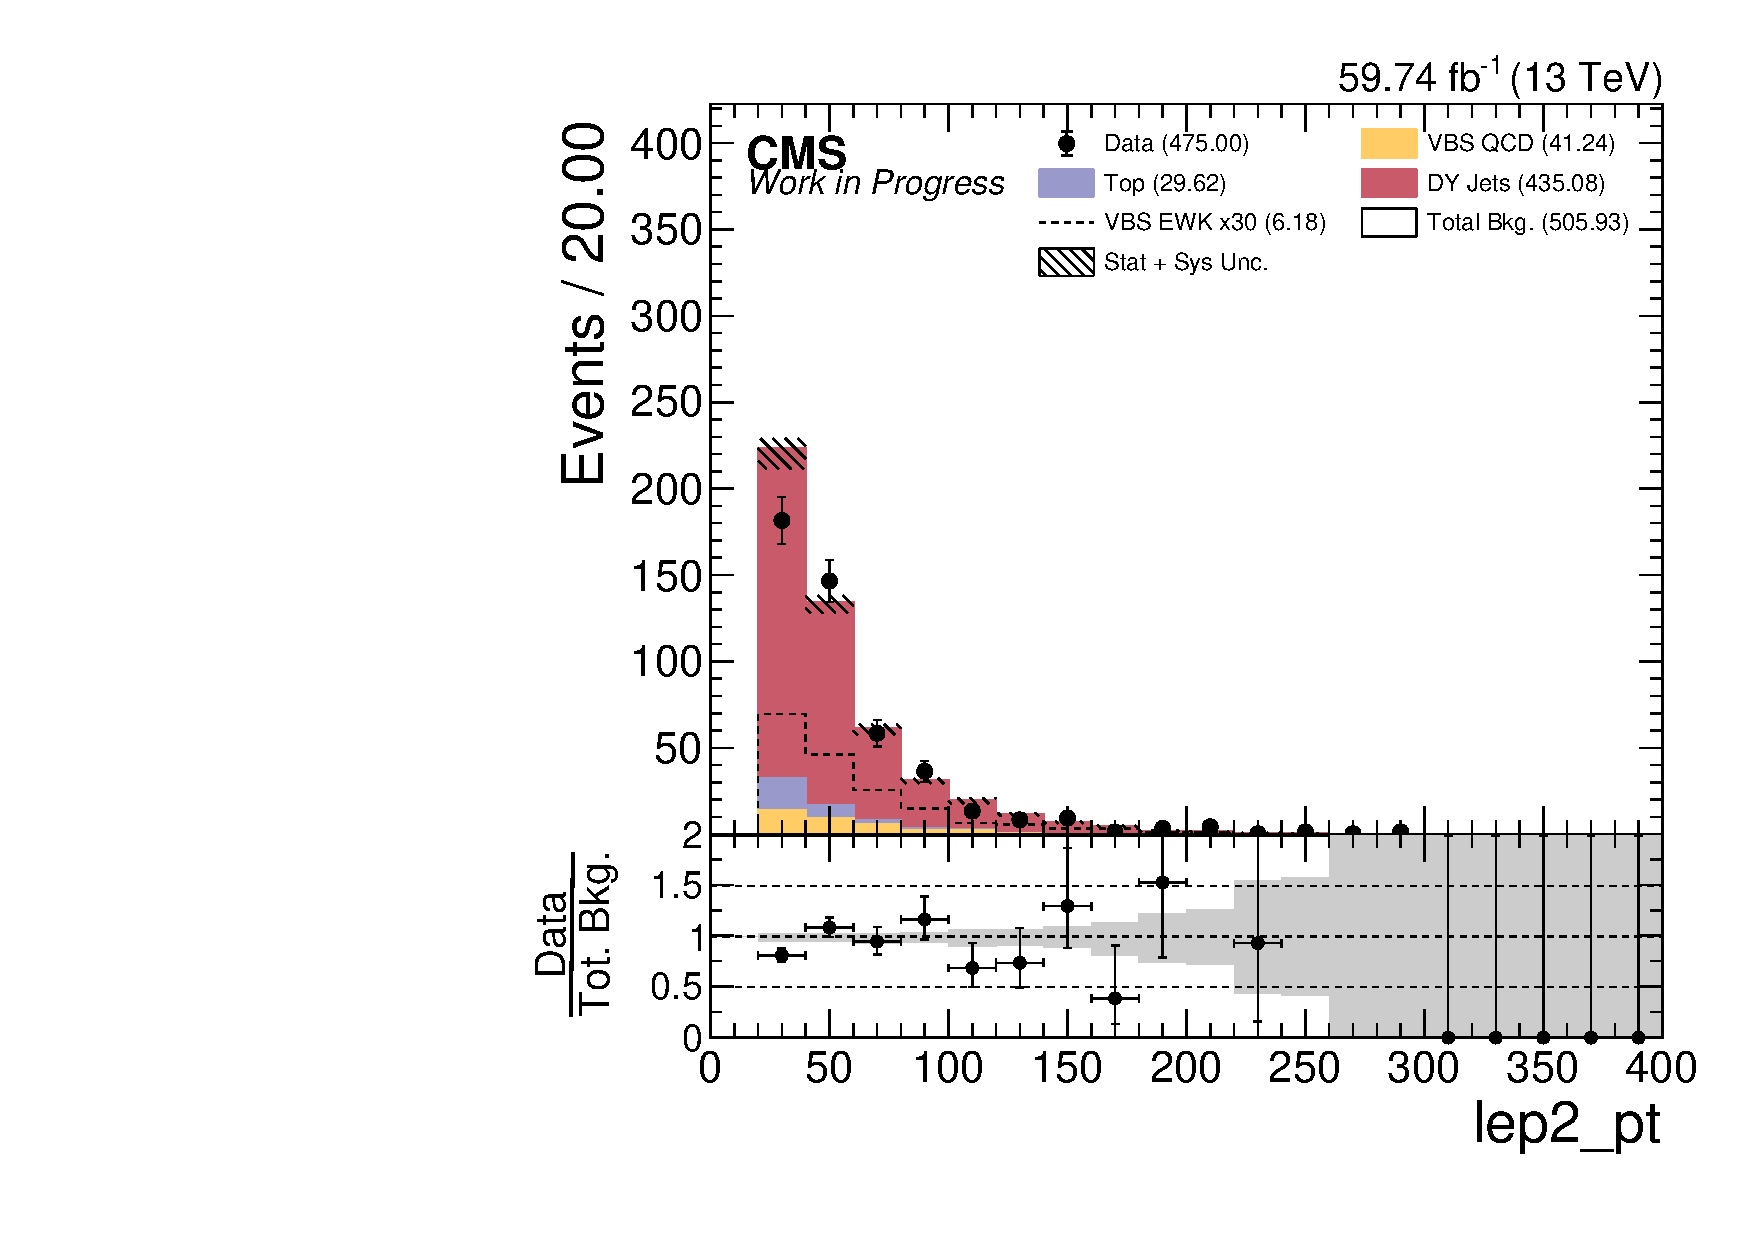
\includegraphics[width=0.30\textwidth]{analysis_plots/2018_zv/cr_vjets_m/lep2_pt.pdf} \\
  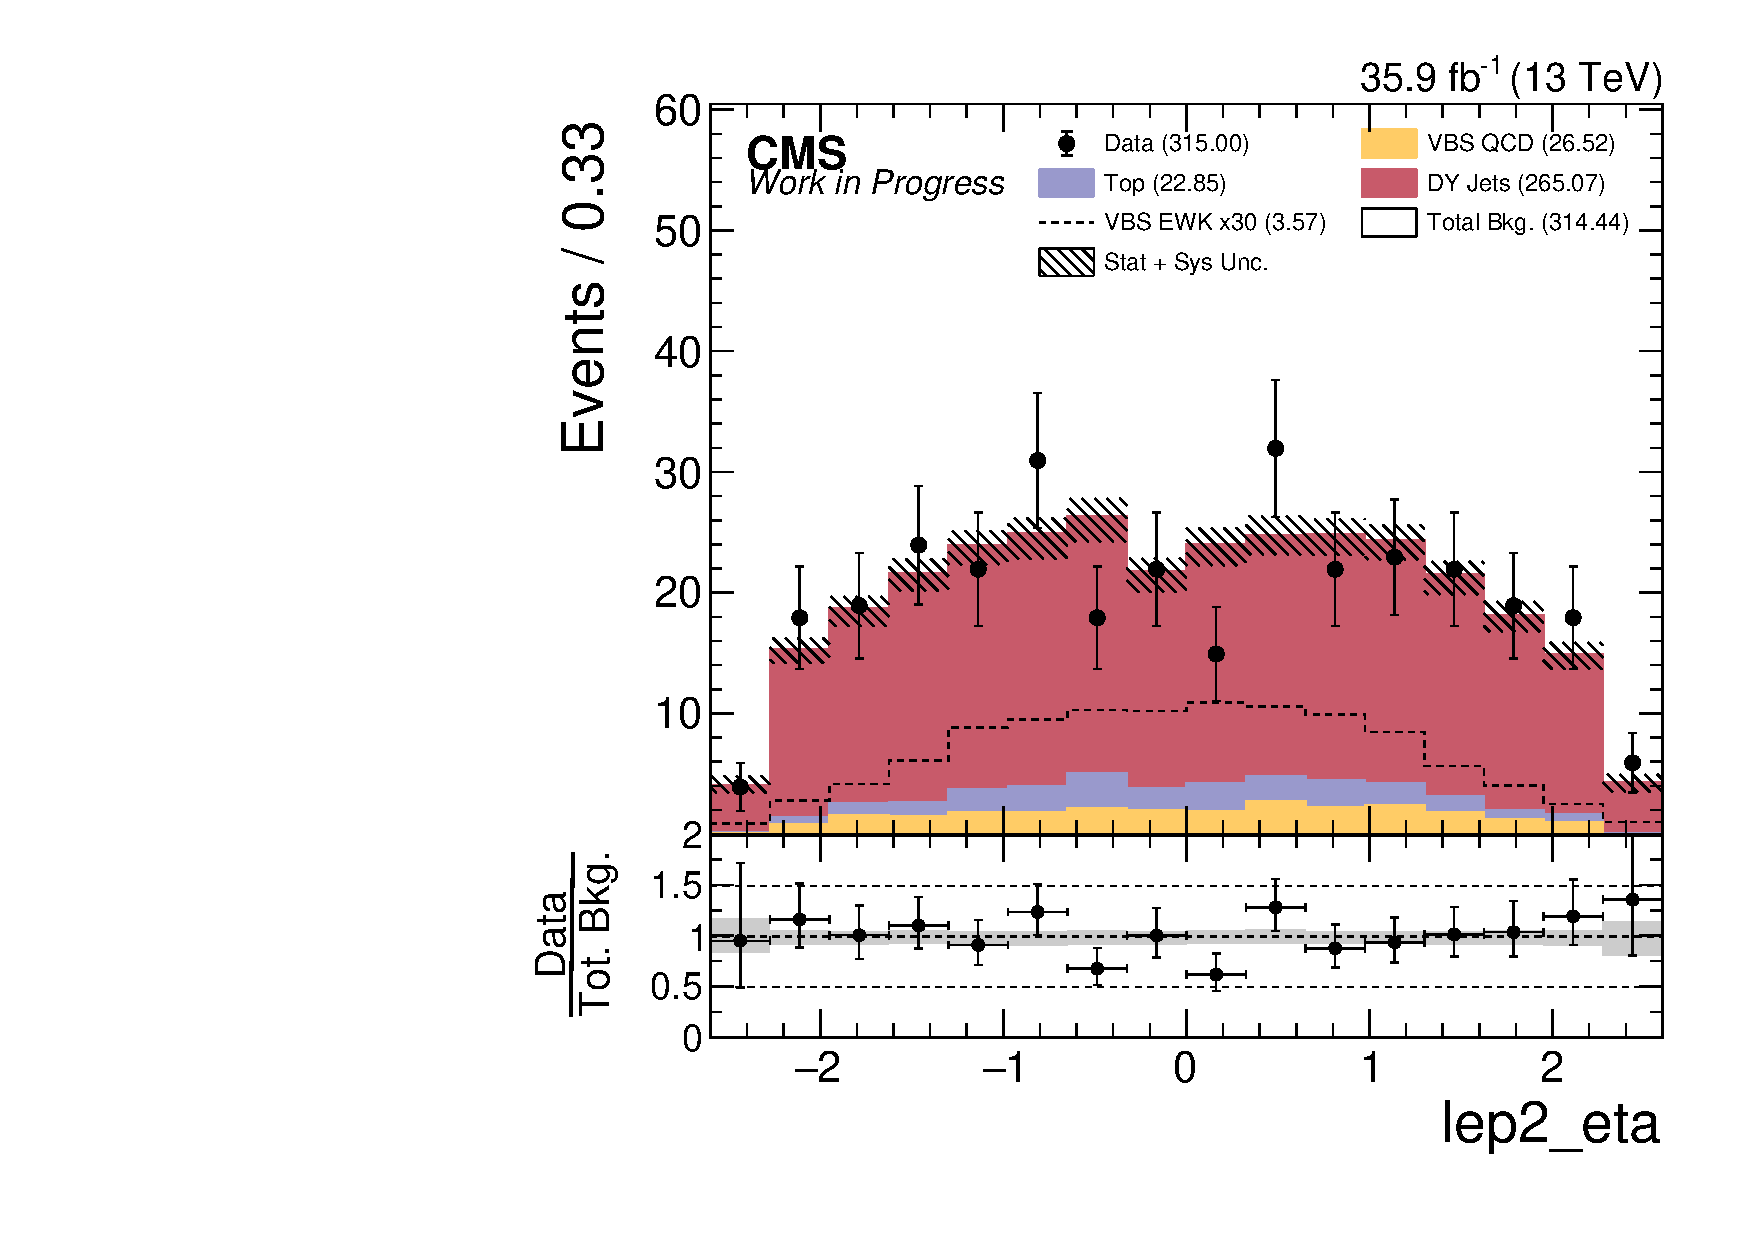
\includegraphics[width=0.30\textwidth]{analysis_plots/2016_zv/cr_vjets_m/lep2_eta.pdf}
  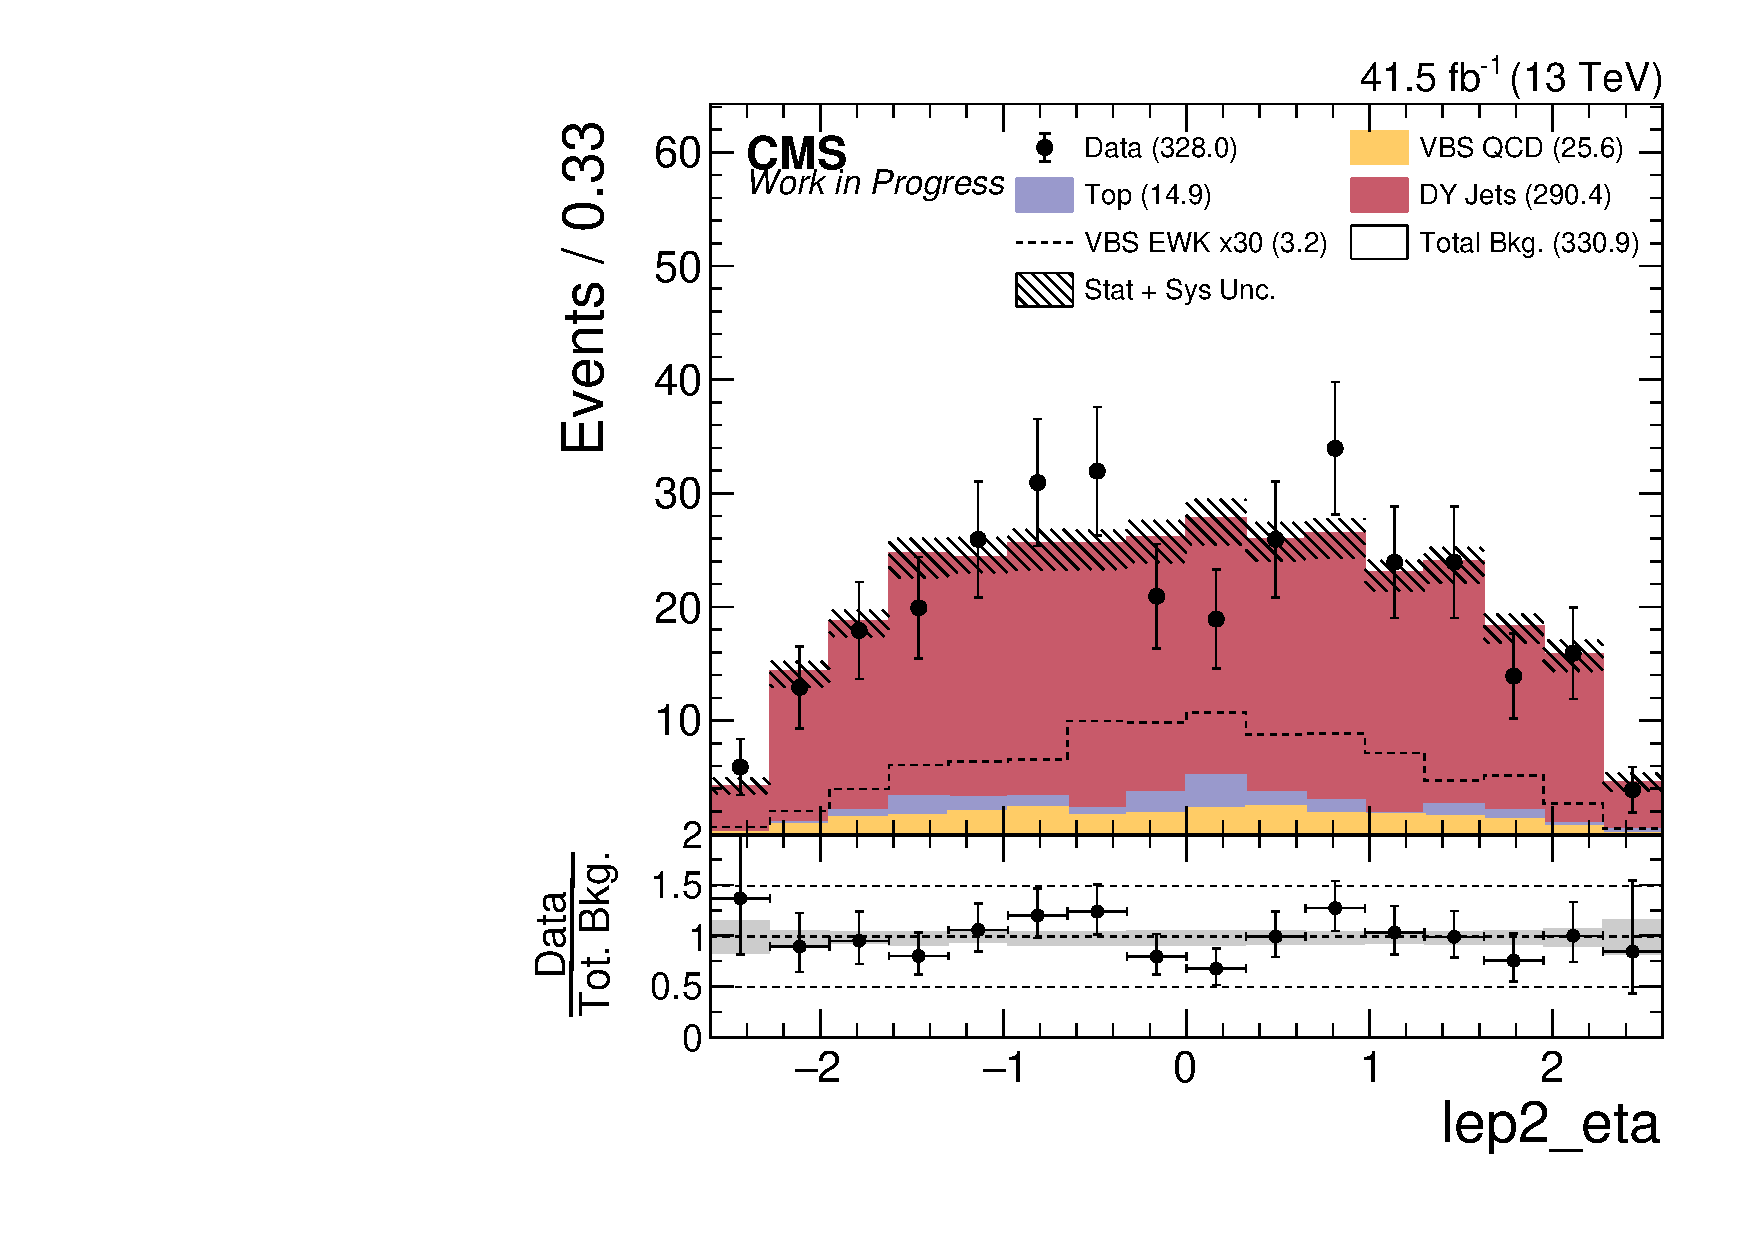
\includegraphics[width=0.30\textwidth]{analysis_plots/2017_zv/cr_vjets_m/lep2_eta.pdf}
  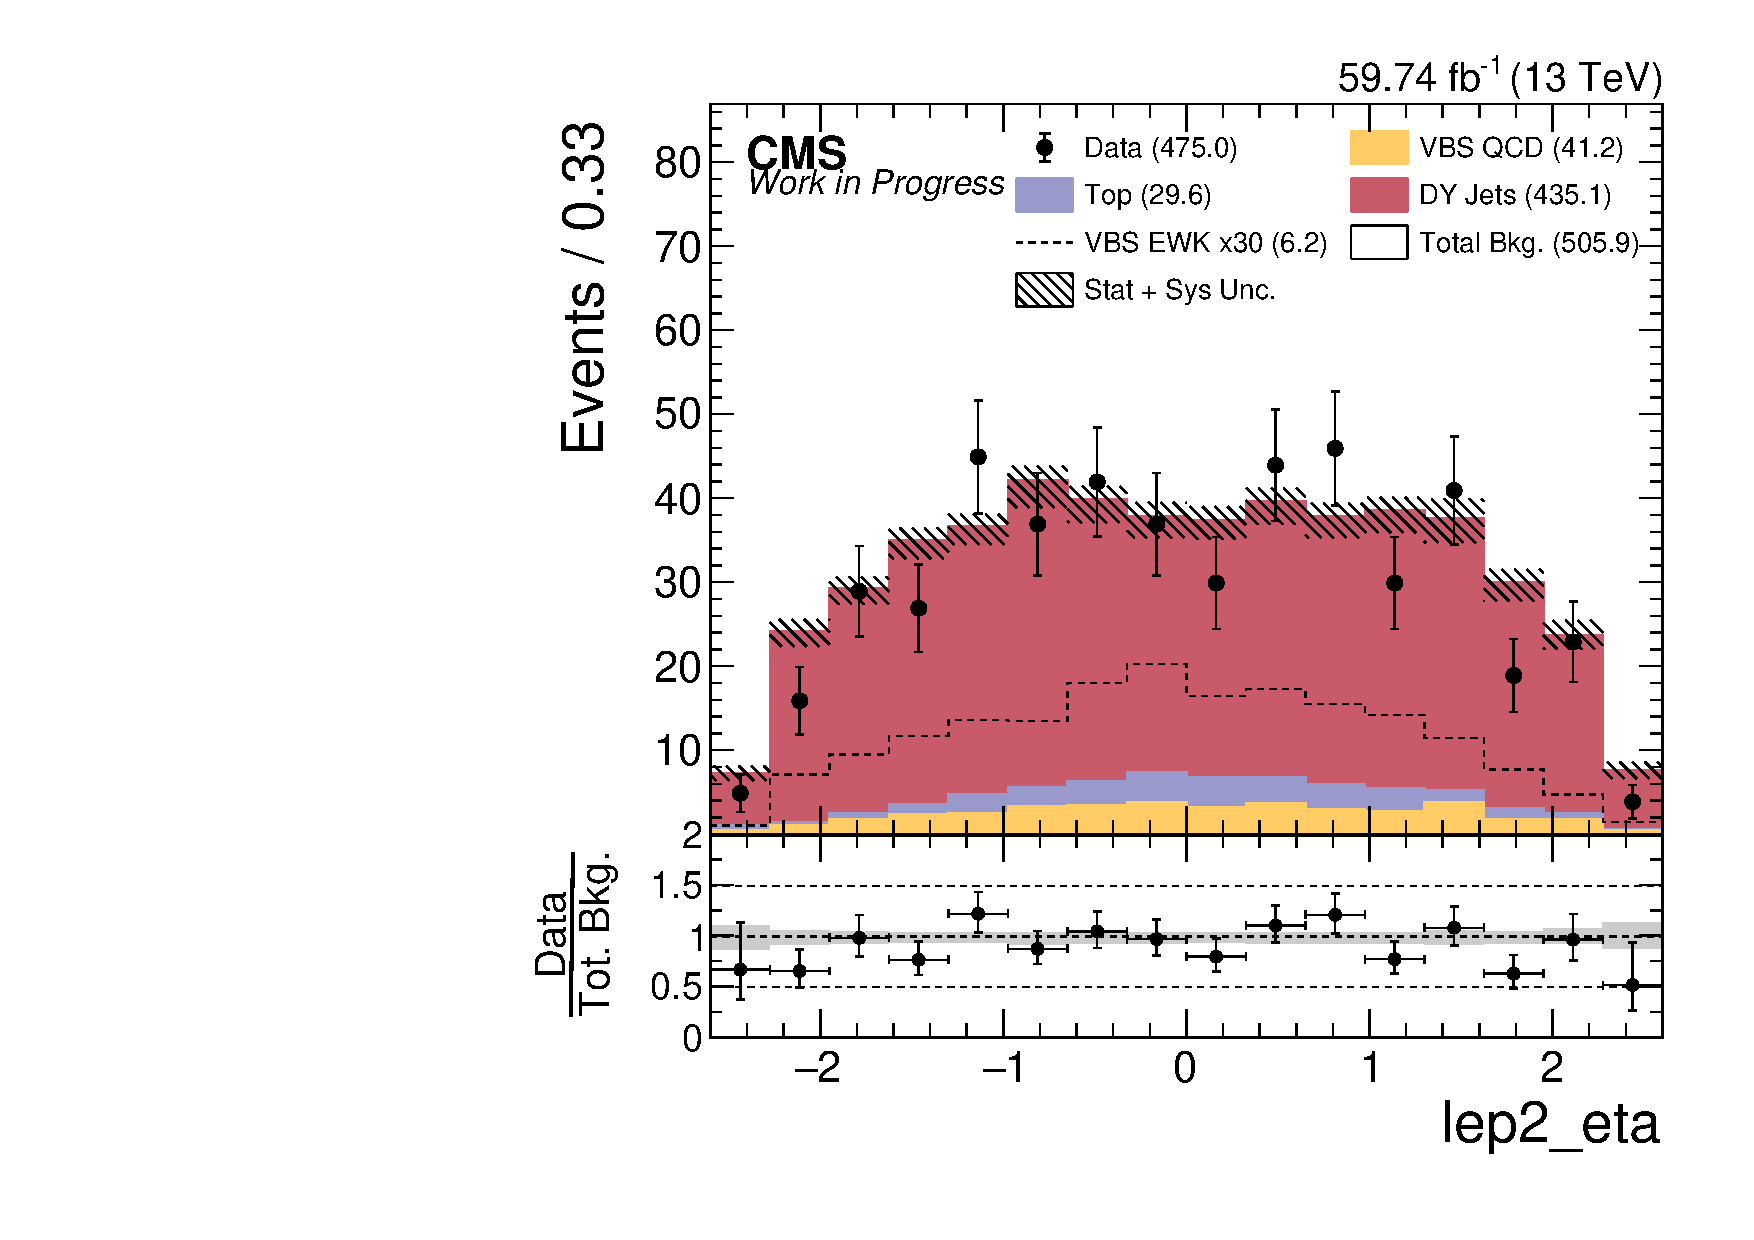
\includegraphics[width=0.30\textwidth]{analysis_plots/2018_zv/cr_vjets_m/lep2_eta.pdf} \\
  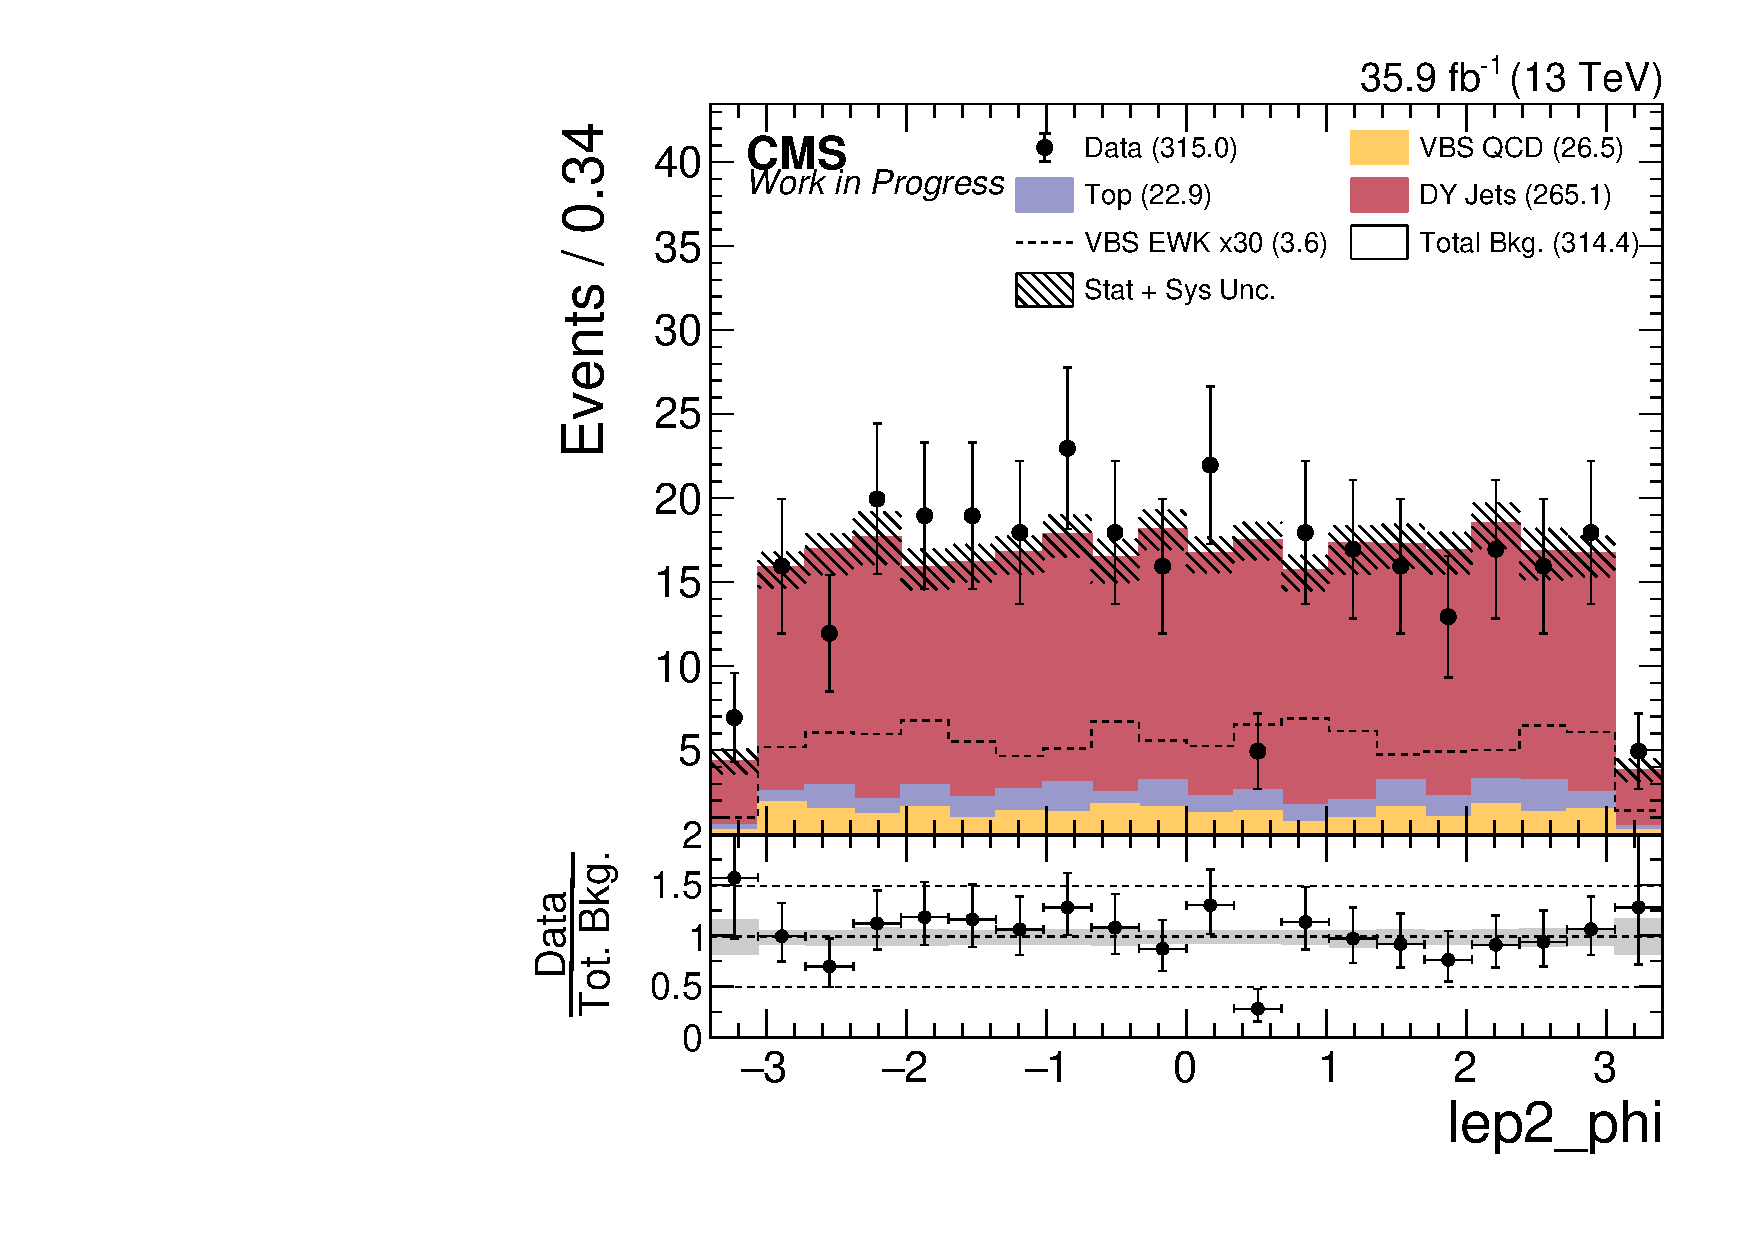
\includegraphics[width=0.30\textwidth]{analysis_plots/2016_zv/cr_vjets_m/lep2_phi.pdf}
  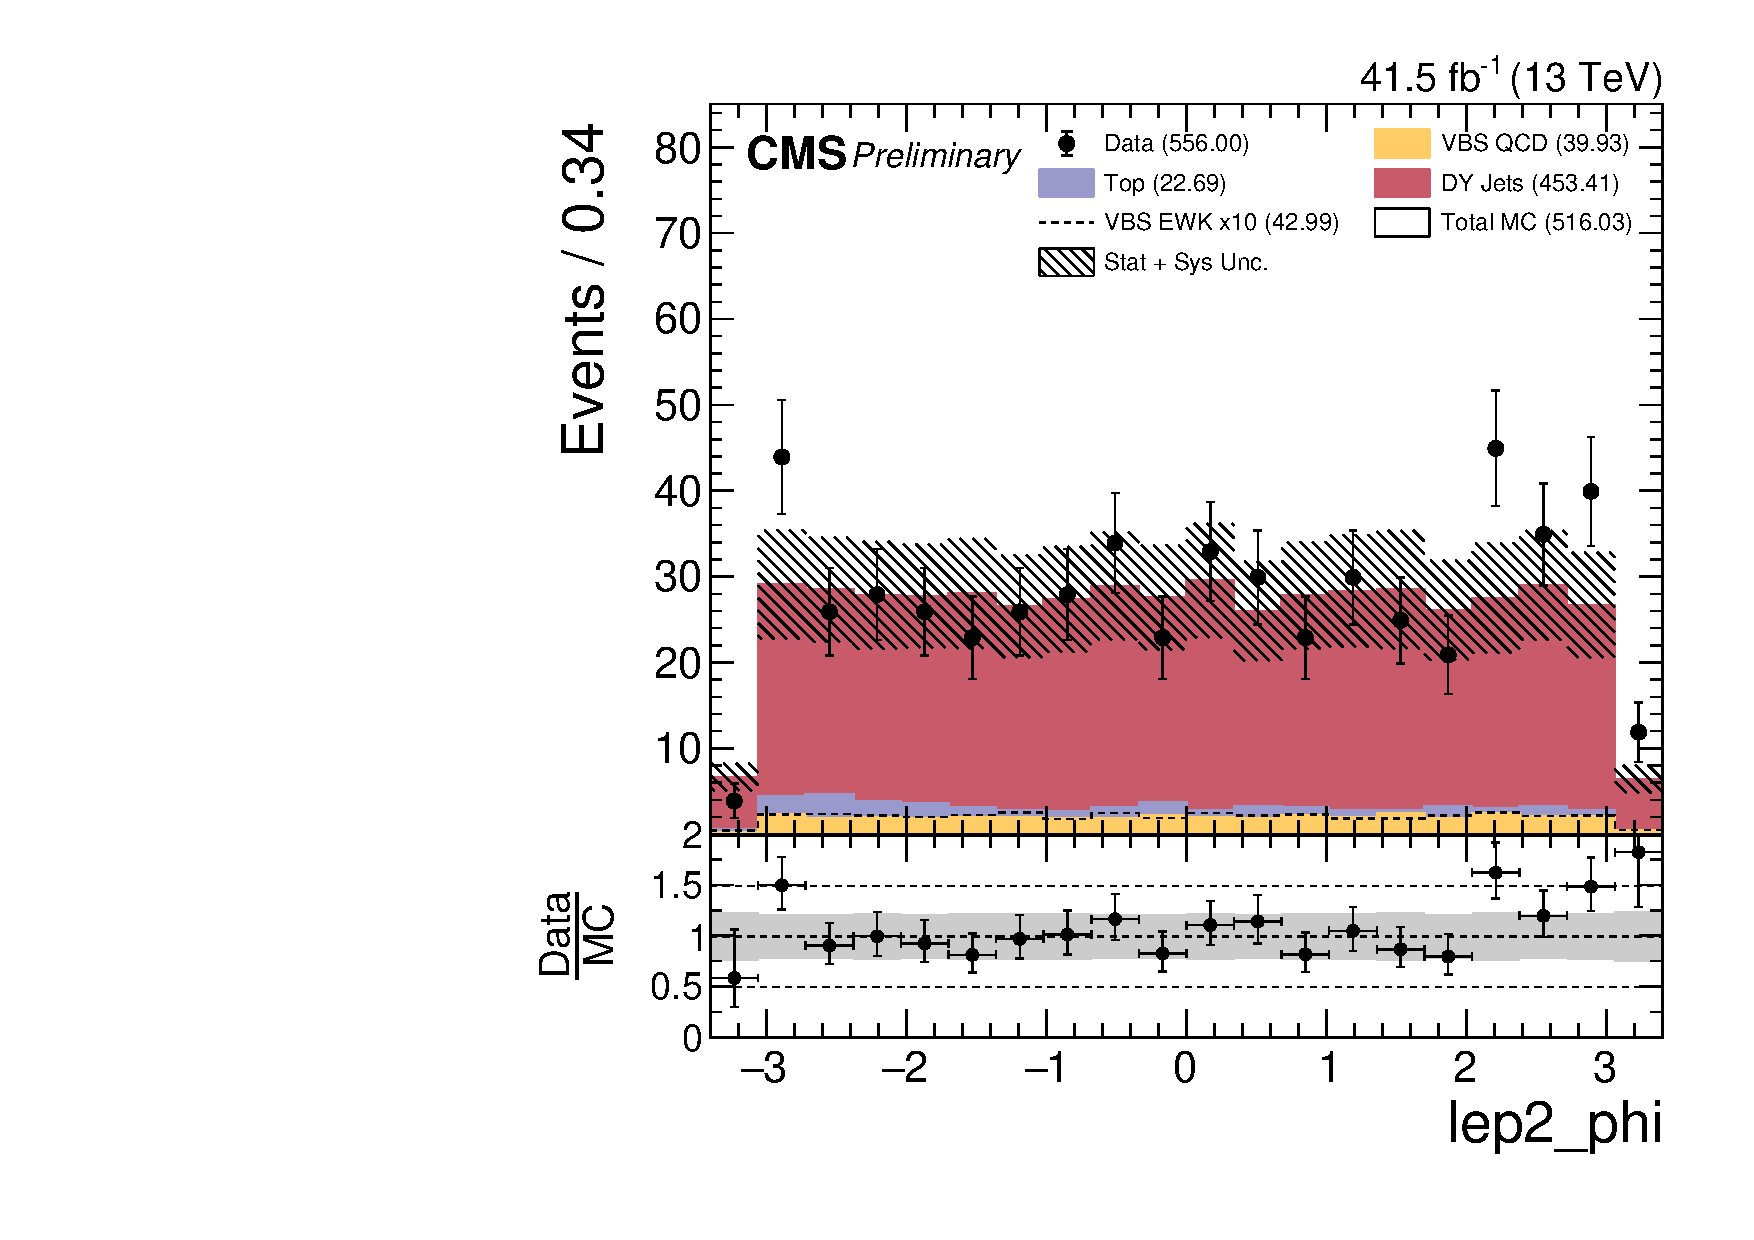
\includegraphics[width=0.30\textwidth]{analysis_plots/2017_zv/cr_vjets_m/lep2_phi.pdf}
  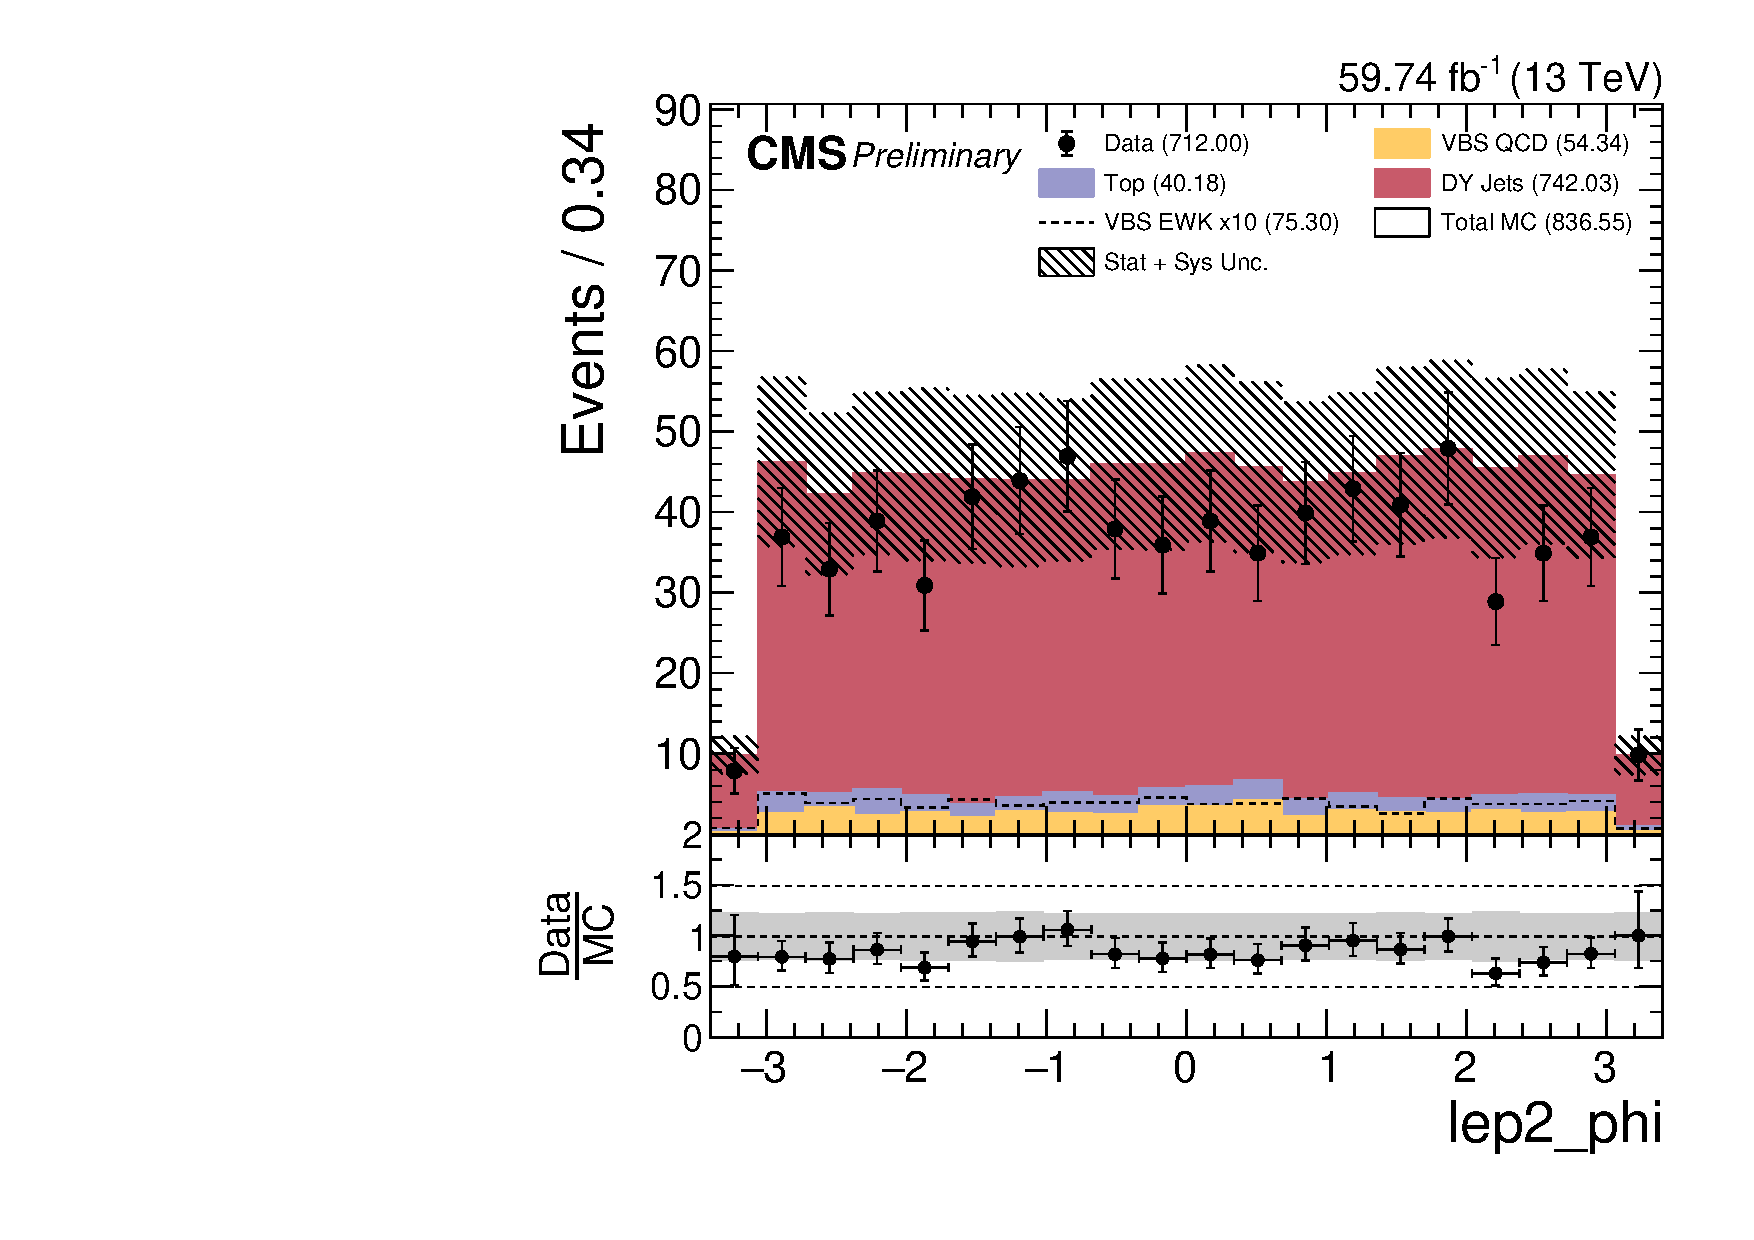
\includegraphics[width=0.30\textwidth]{analysis_plots/2018_zv/cr_vjets_m/lep2_phi.pdf} \\
  \caption[DY+Jets Control Region: Trailing muon kinematics in Boosted ZV Channel]%
  {DY+Jets Control Region: Trailing muon kinematics in Boosted ZV Channel. From Left to Right: 2016,
    2017, and 2018. From Top to Bottom: \( p_T \), \( \eta \), \( \phi \).}%
  \label{fig:zv-cr-vjets-m-lep2-pt-eta-phi}
\end{figure}

\begin{figure}[!ht]
  \centering
  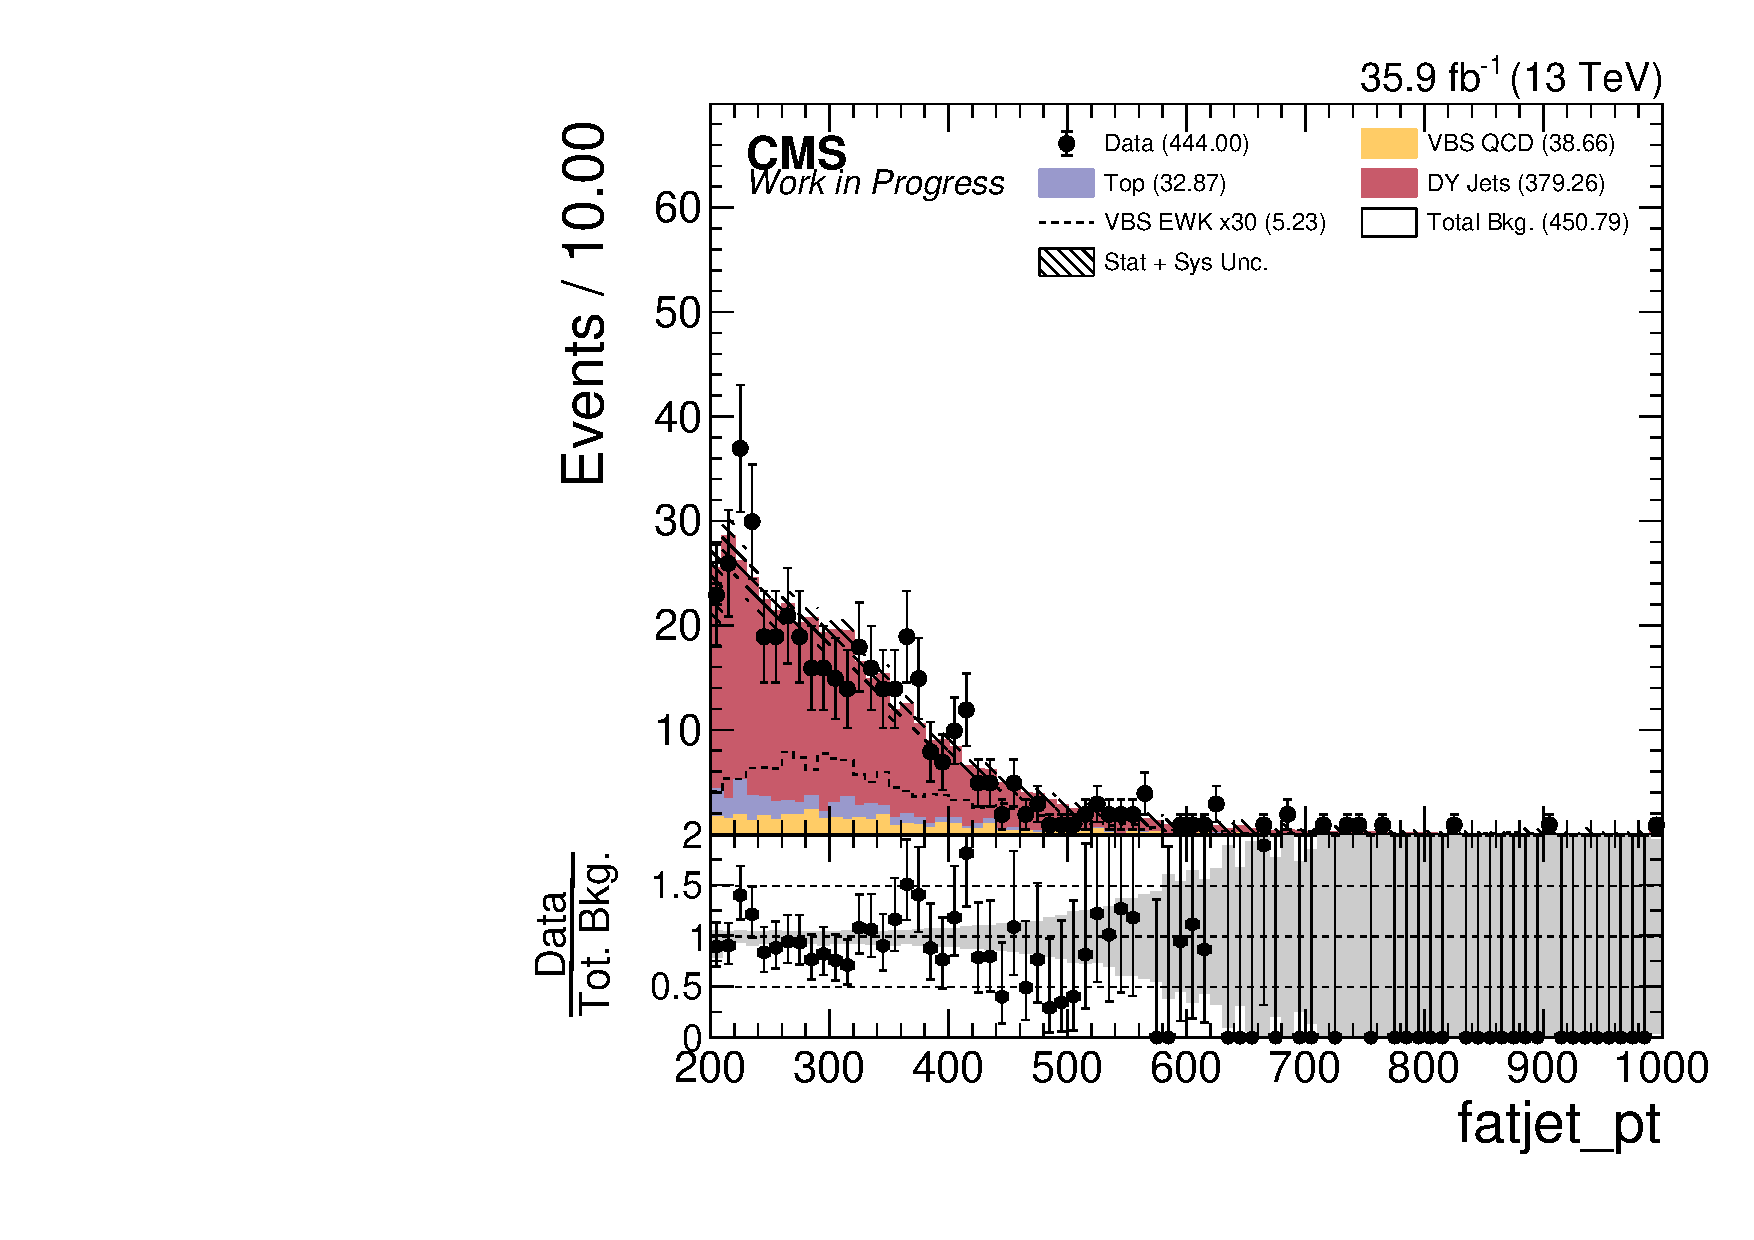
\includegraphics[width=0.30\textwidth]{analysis_plots/2016_zv/cr_vjets_l/fatjet_pt.pdf}
  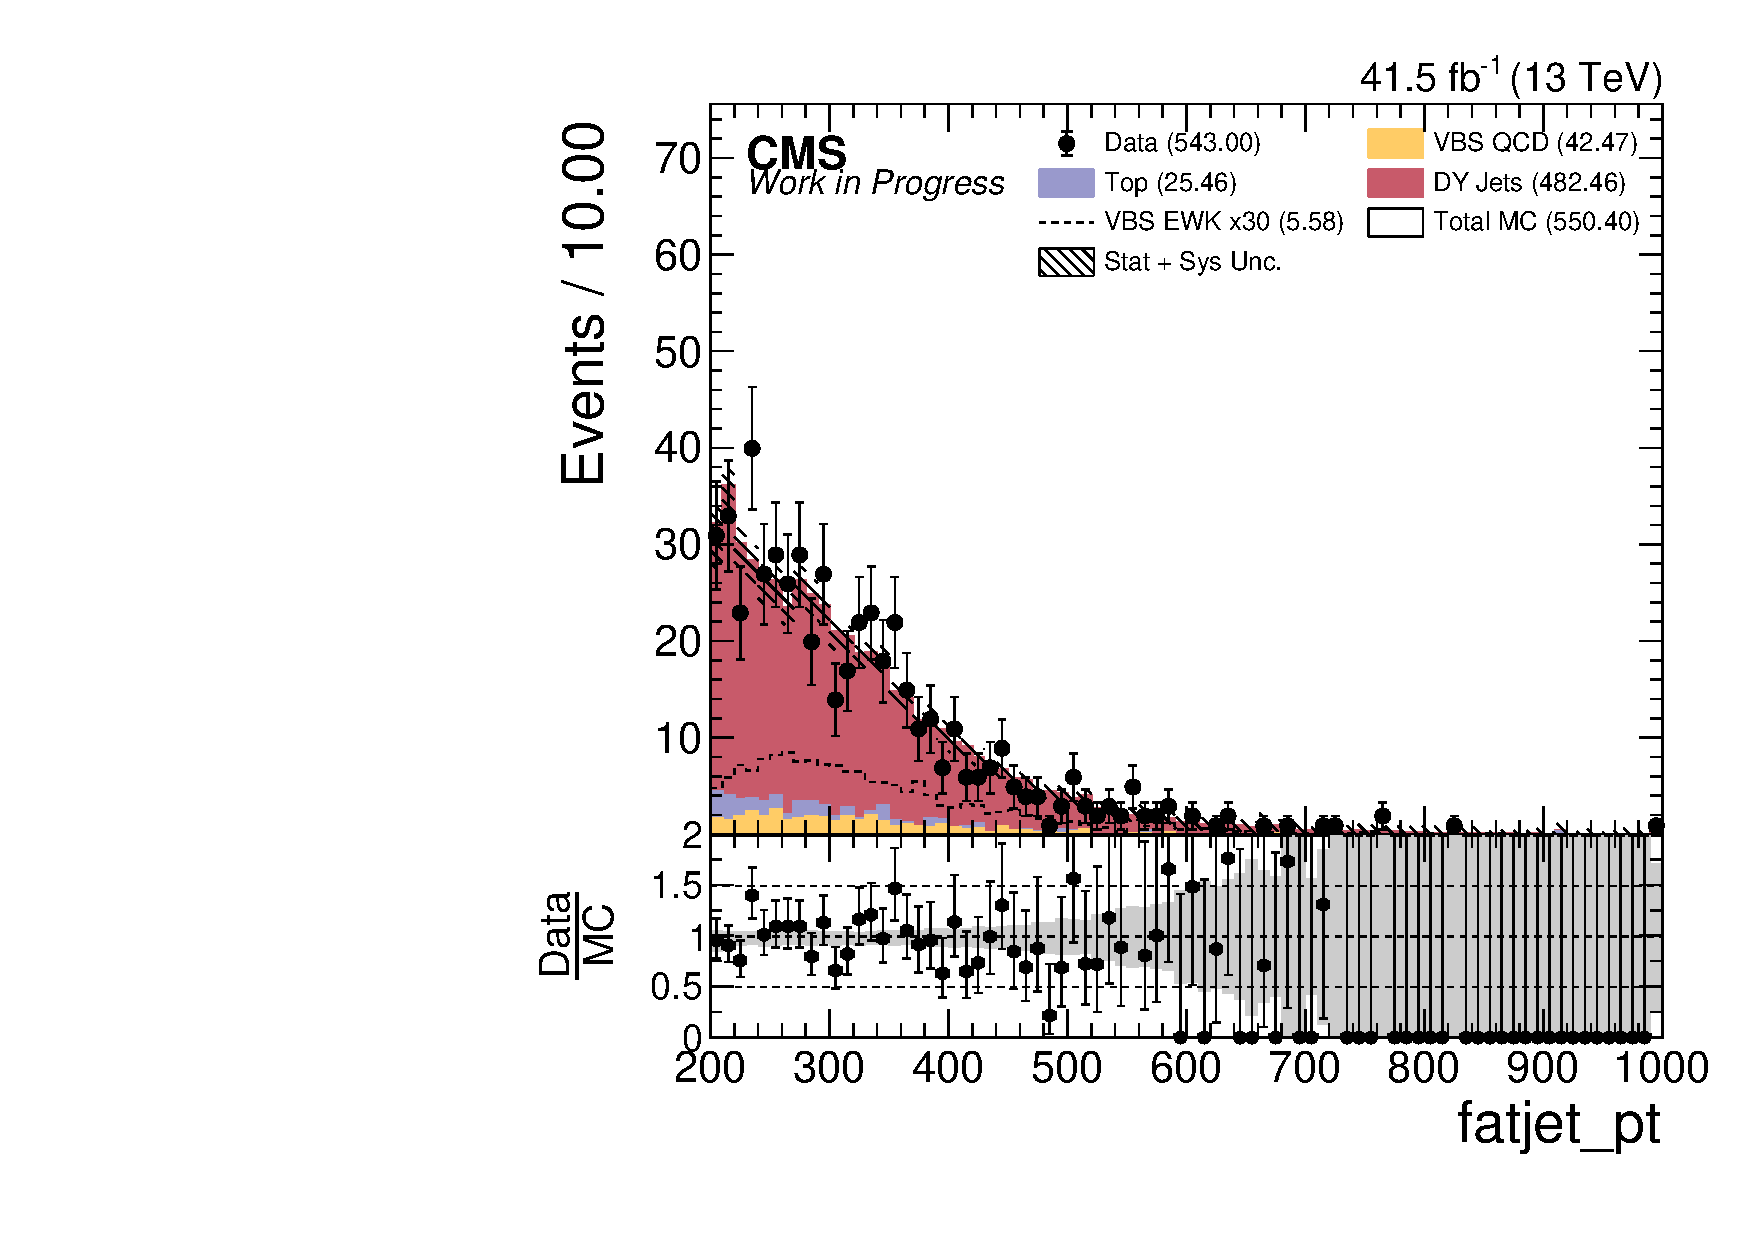
\includegraphics[width=0.30\textwidth]{analysis_plots/2017_zv/cr_vjets_l/fatjet_pt.pdf}
  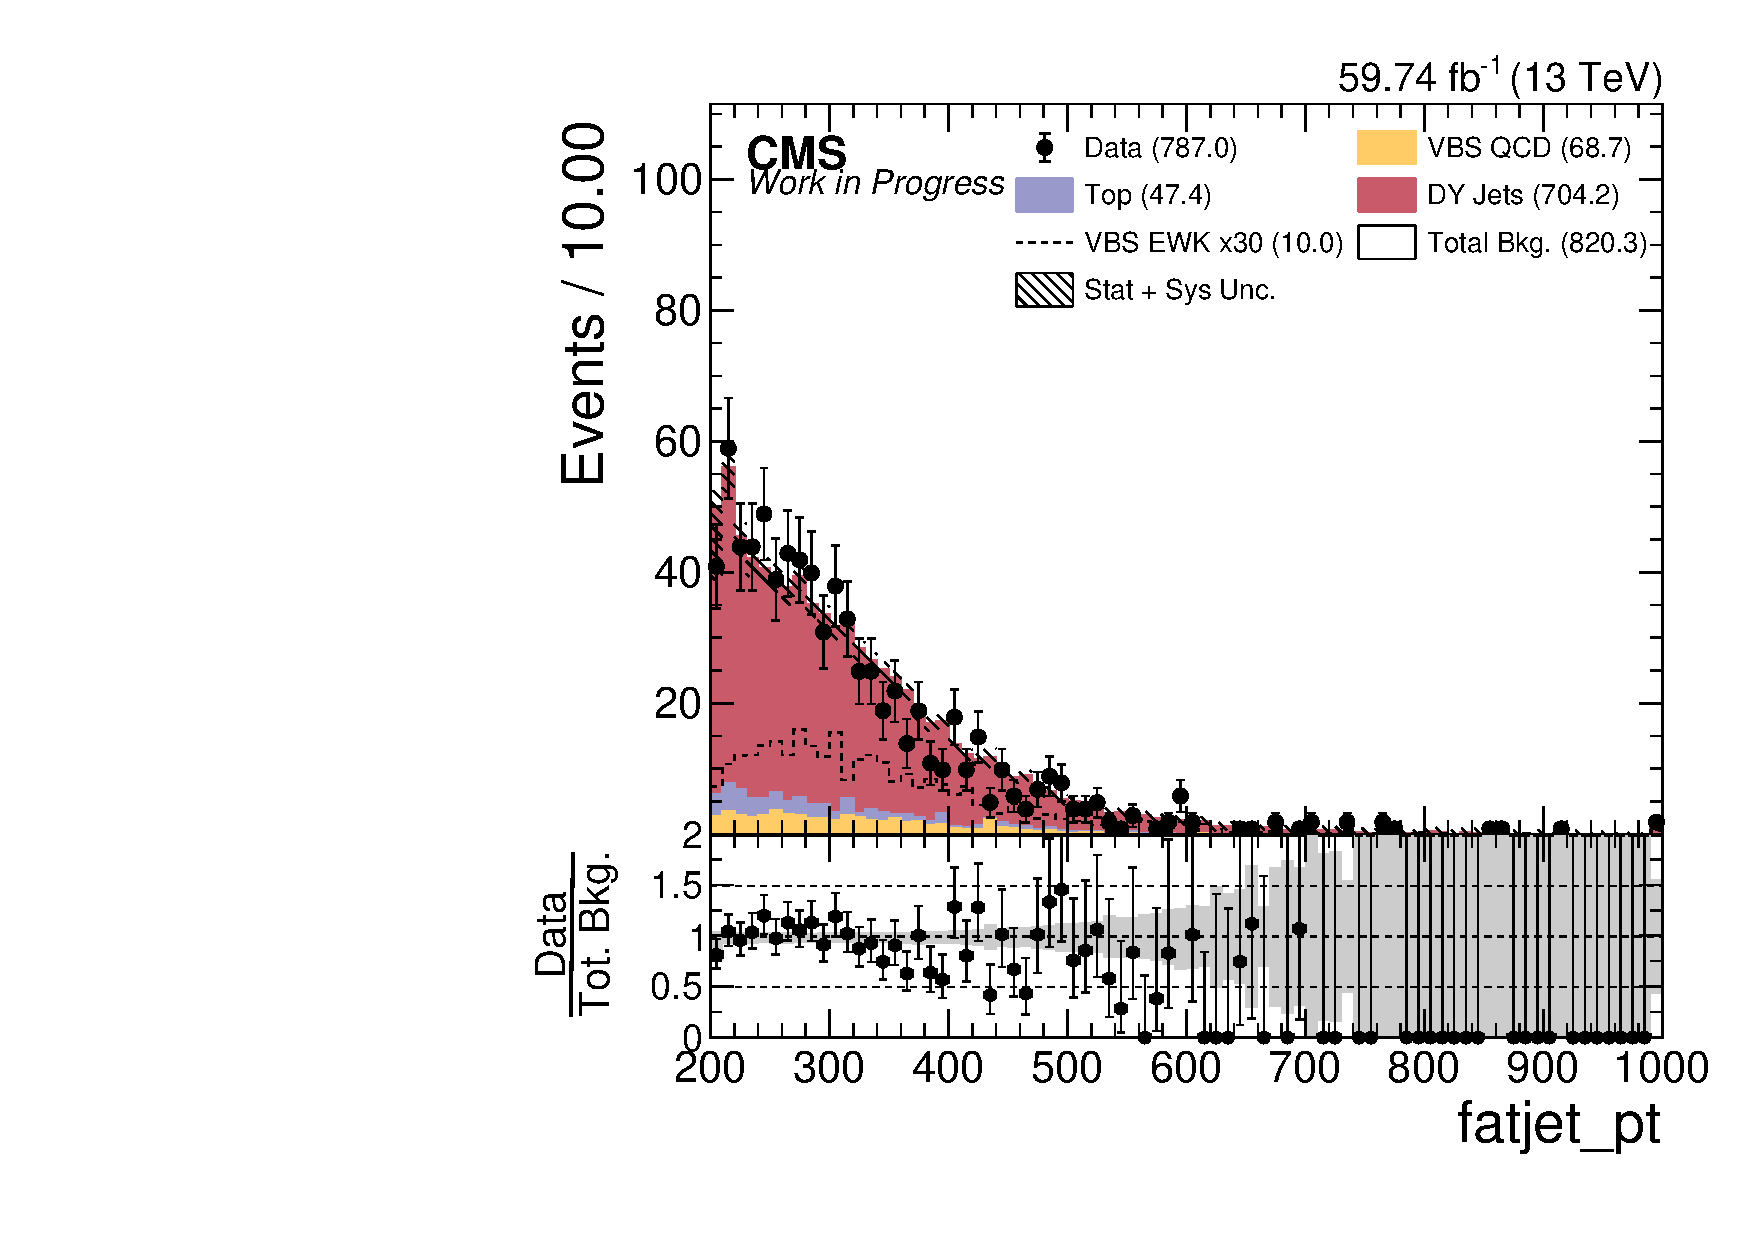
\includegraphics[width=0.30\textwidth]{analysis_plots/2018_zv/cr_vjets_l/fatjet_pt.pdf} \\
  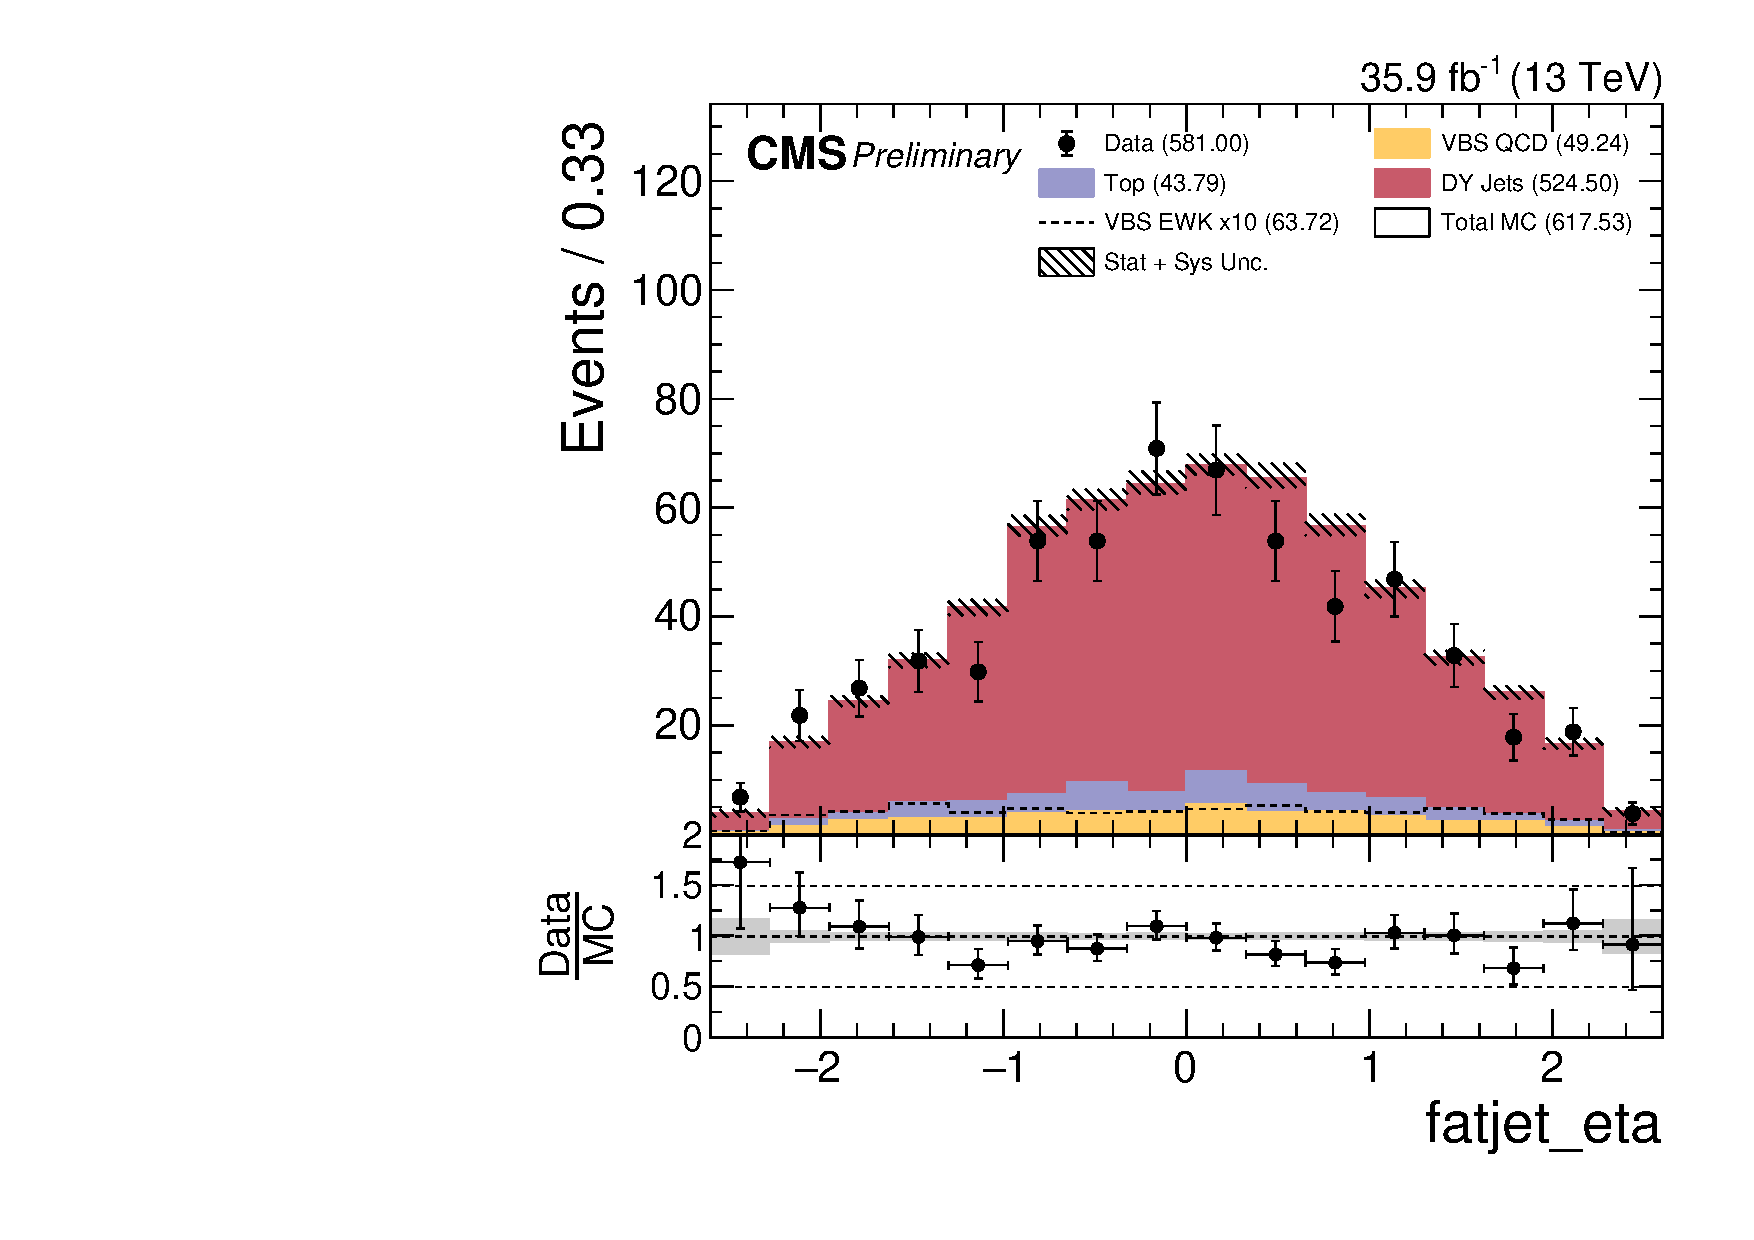
\includegraphics[width=0.30\textwidth]{analysis_plots/2016_zv/cr_vjets_l/fatjet_eta.pdf}
  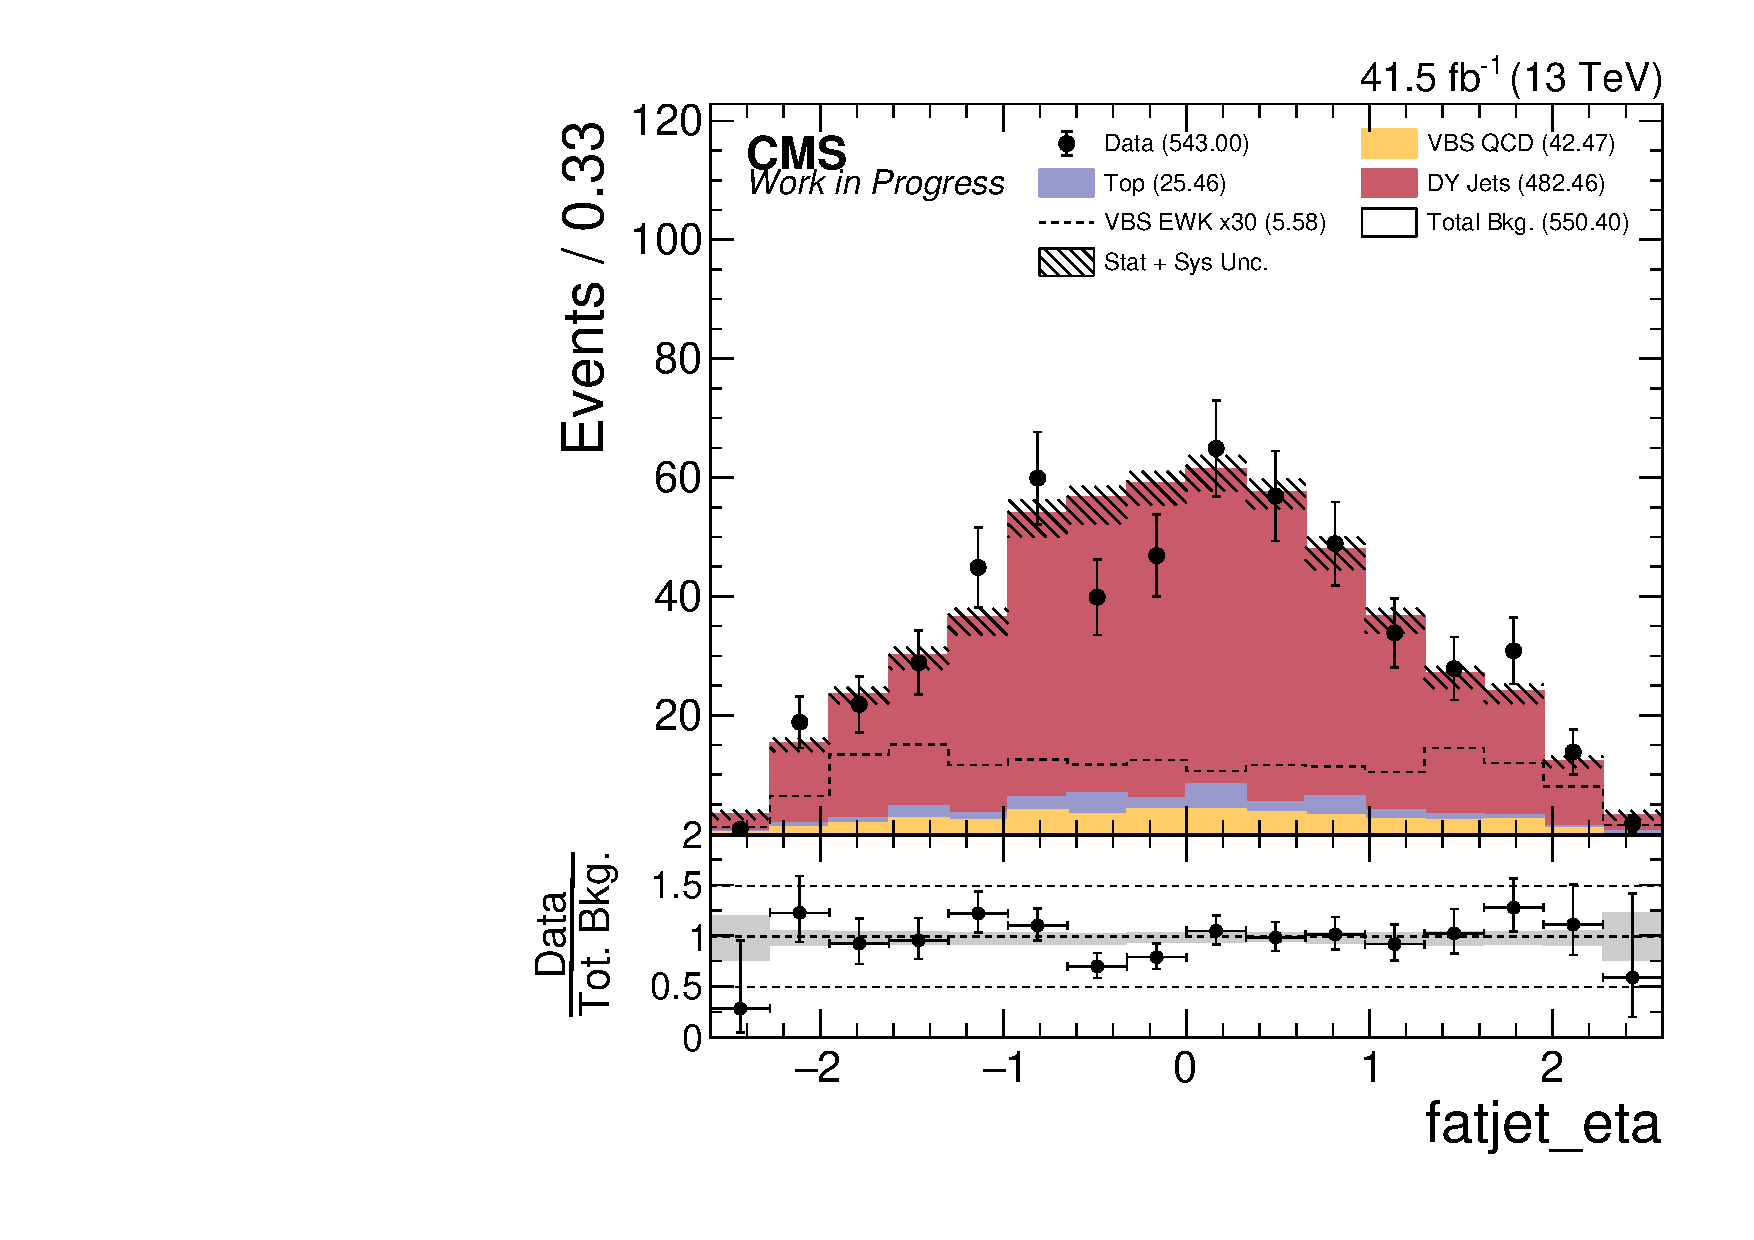
\includegraphics[width=0.30\textwidth]{analysis_plots/2017_zv/cr_vjets_l/fatjet_eta.pdf}
  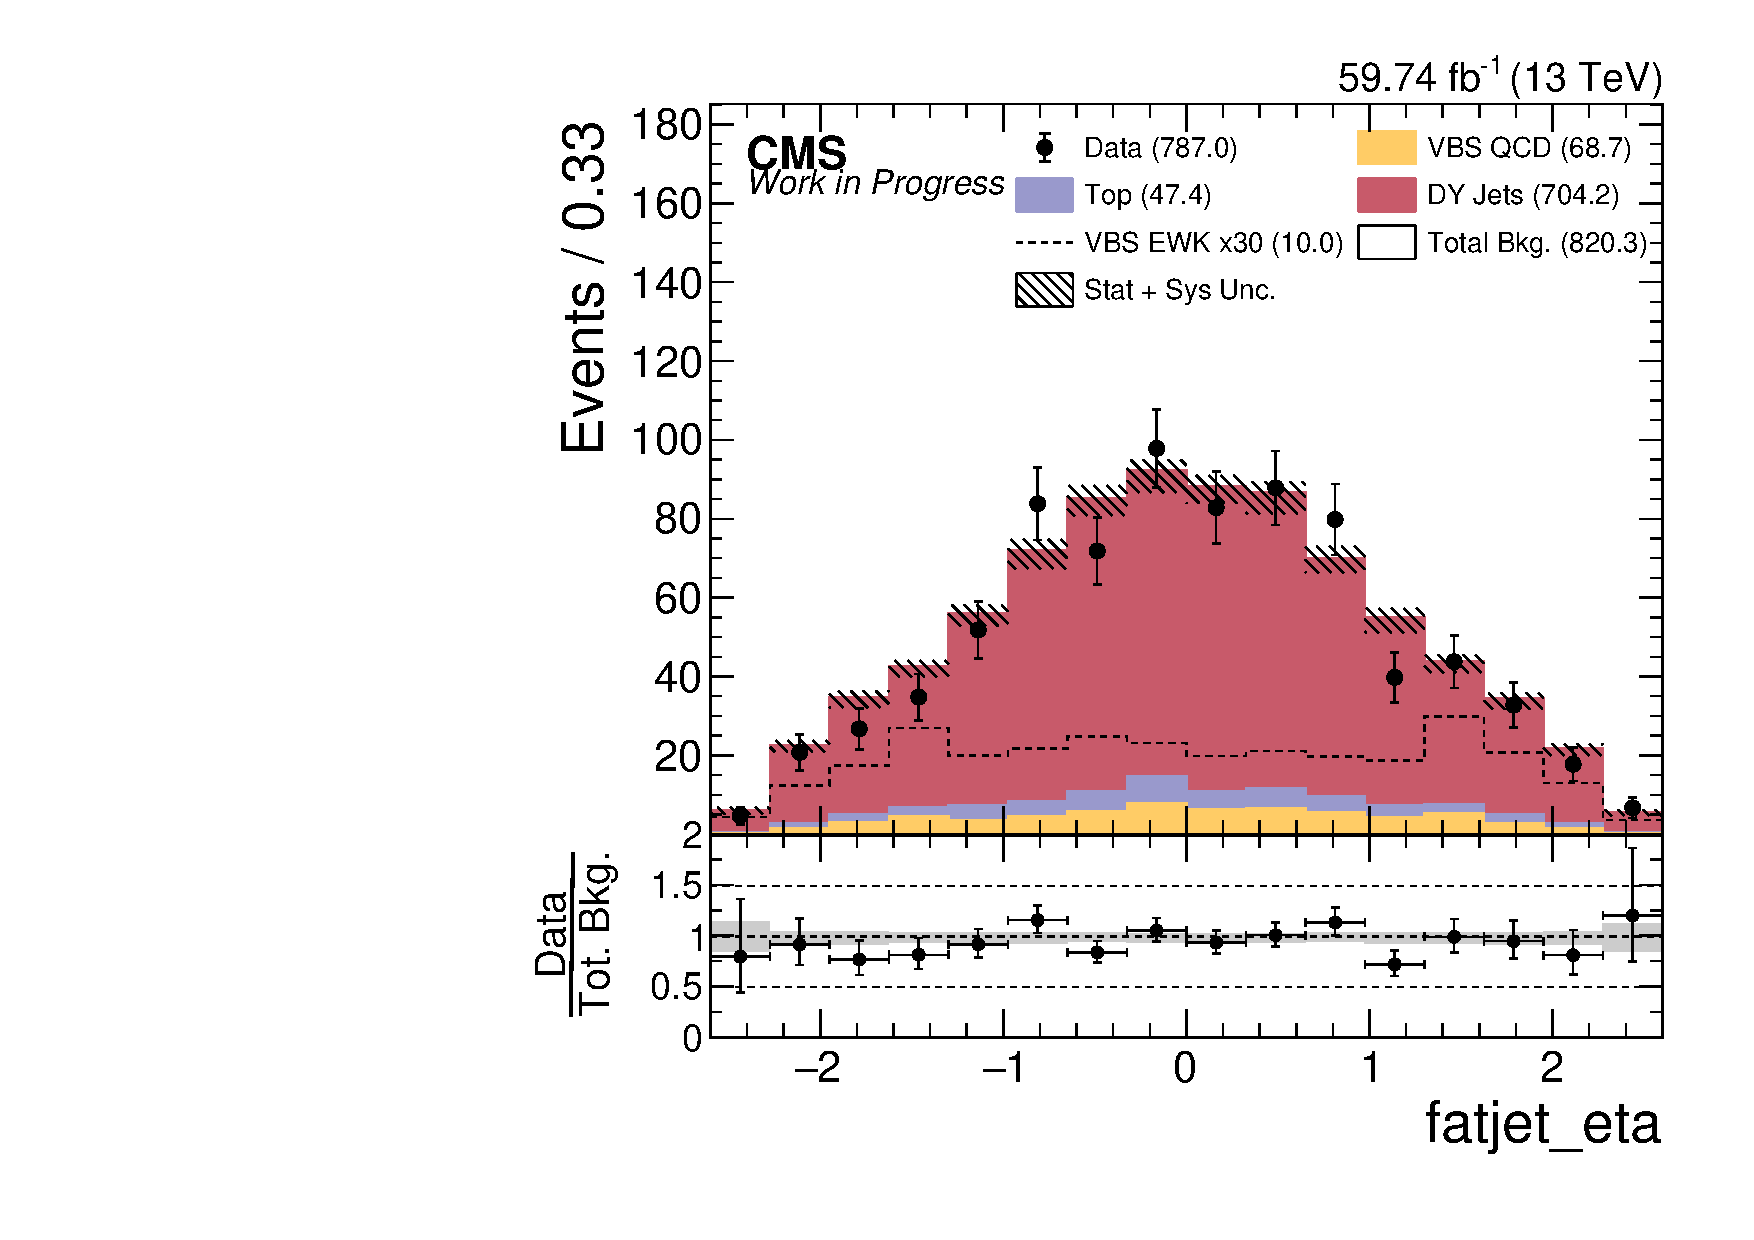
\includegraphics[width=0.30\textwidth]{analysis_plots/2018_zv/cr_vjets_l/fatjet_eta.pdf} \\
  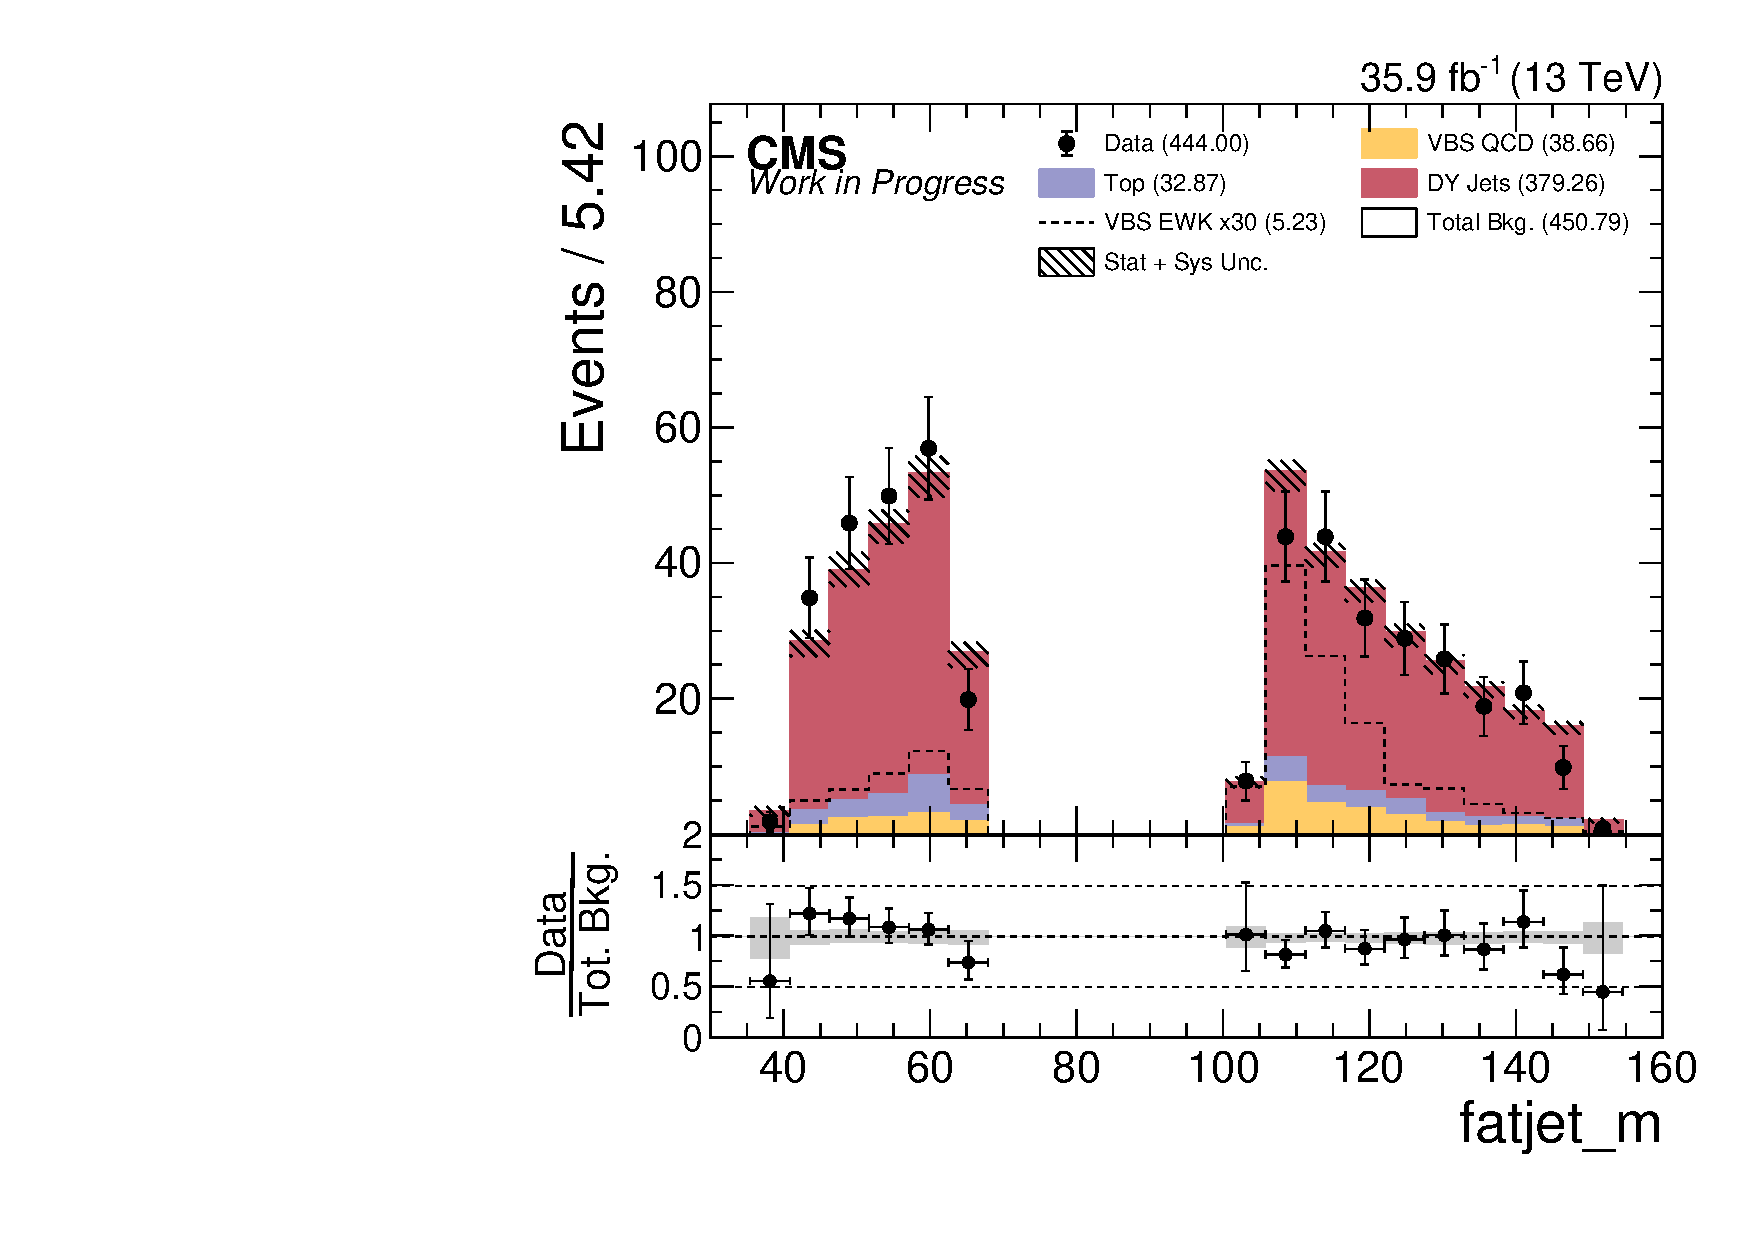
\includegraphics[width=0.30\textwidth]{analysis_plots/2016_zv/cr_vjets_l/fatjet_m.pdf}
  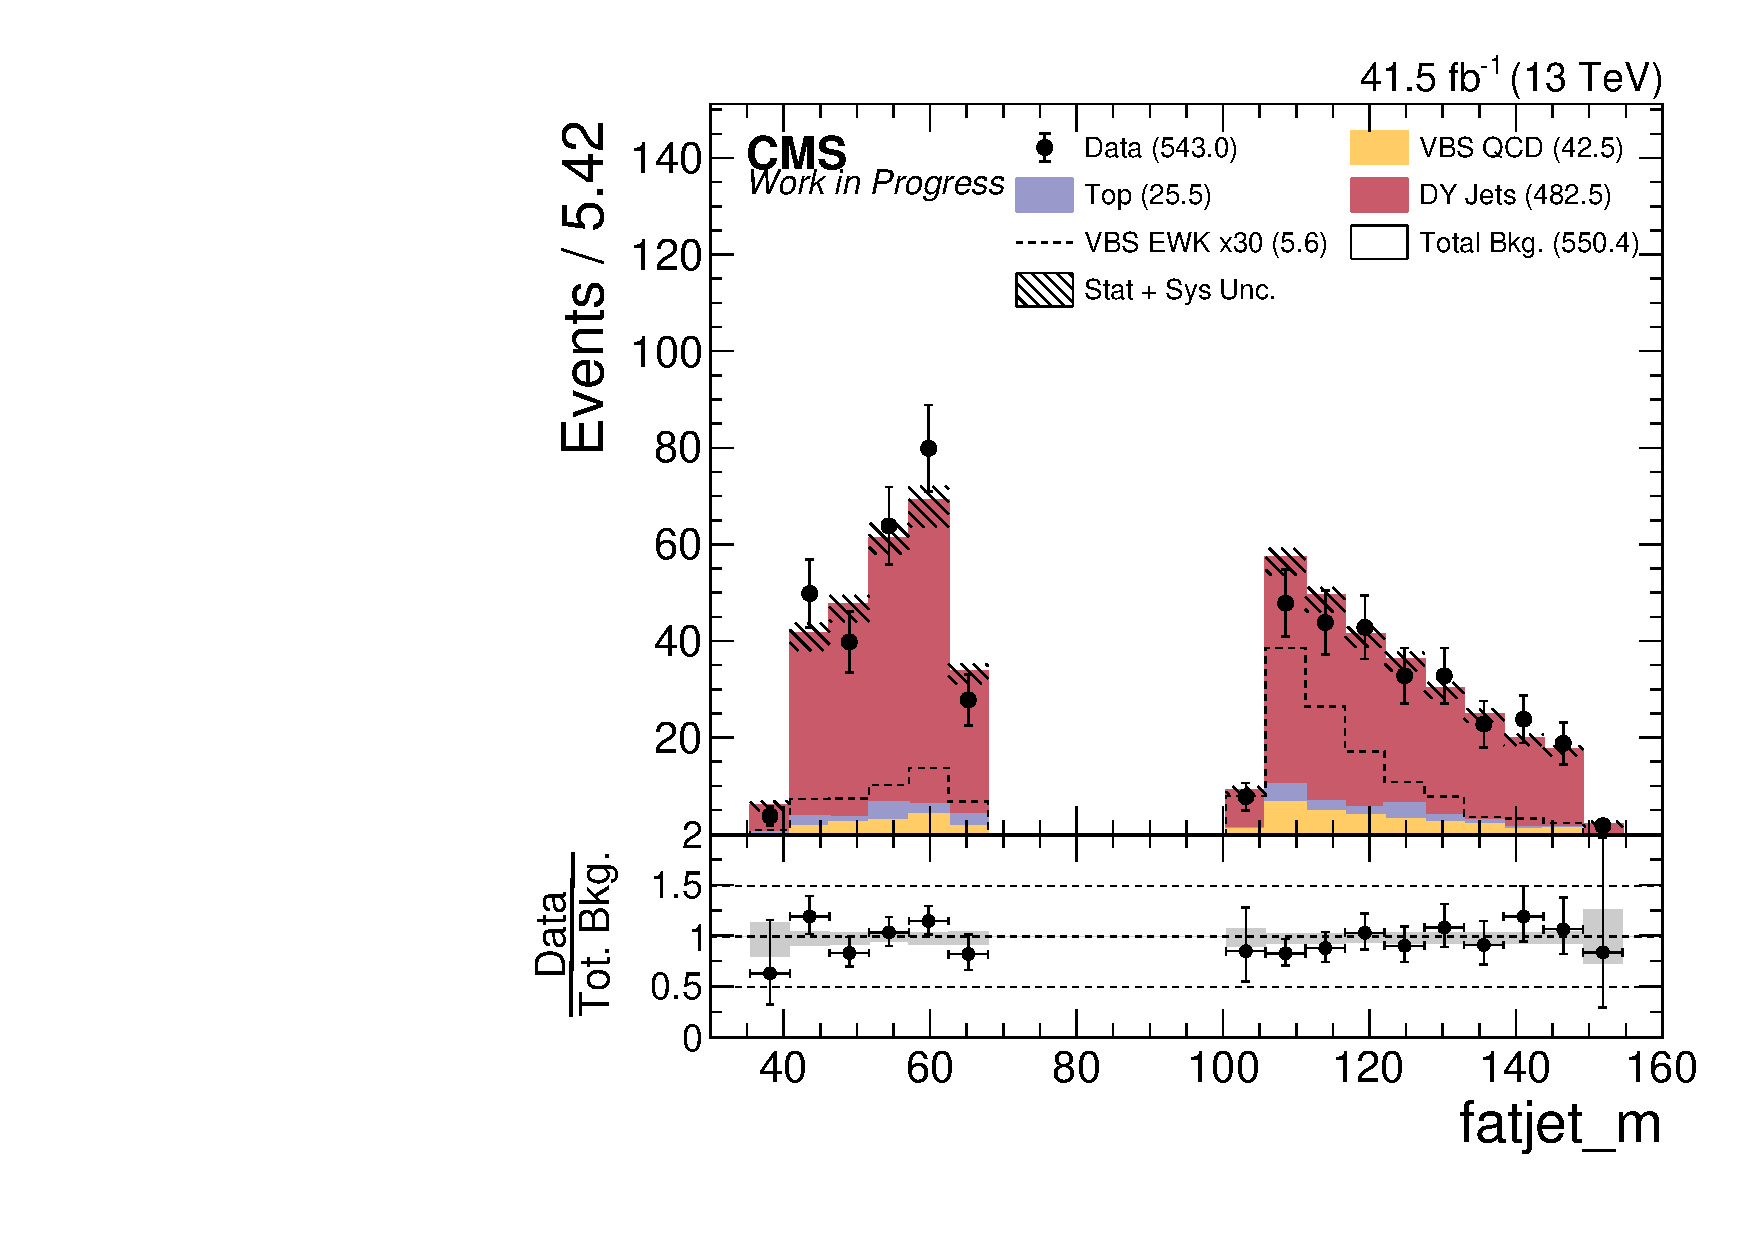
\includegraphics[width=0.30\textwidth]{analysis_plots/2017_zv/cr_vjets_l/fatjet_m.pdf}
  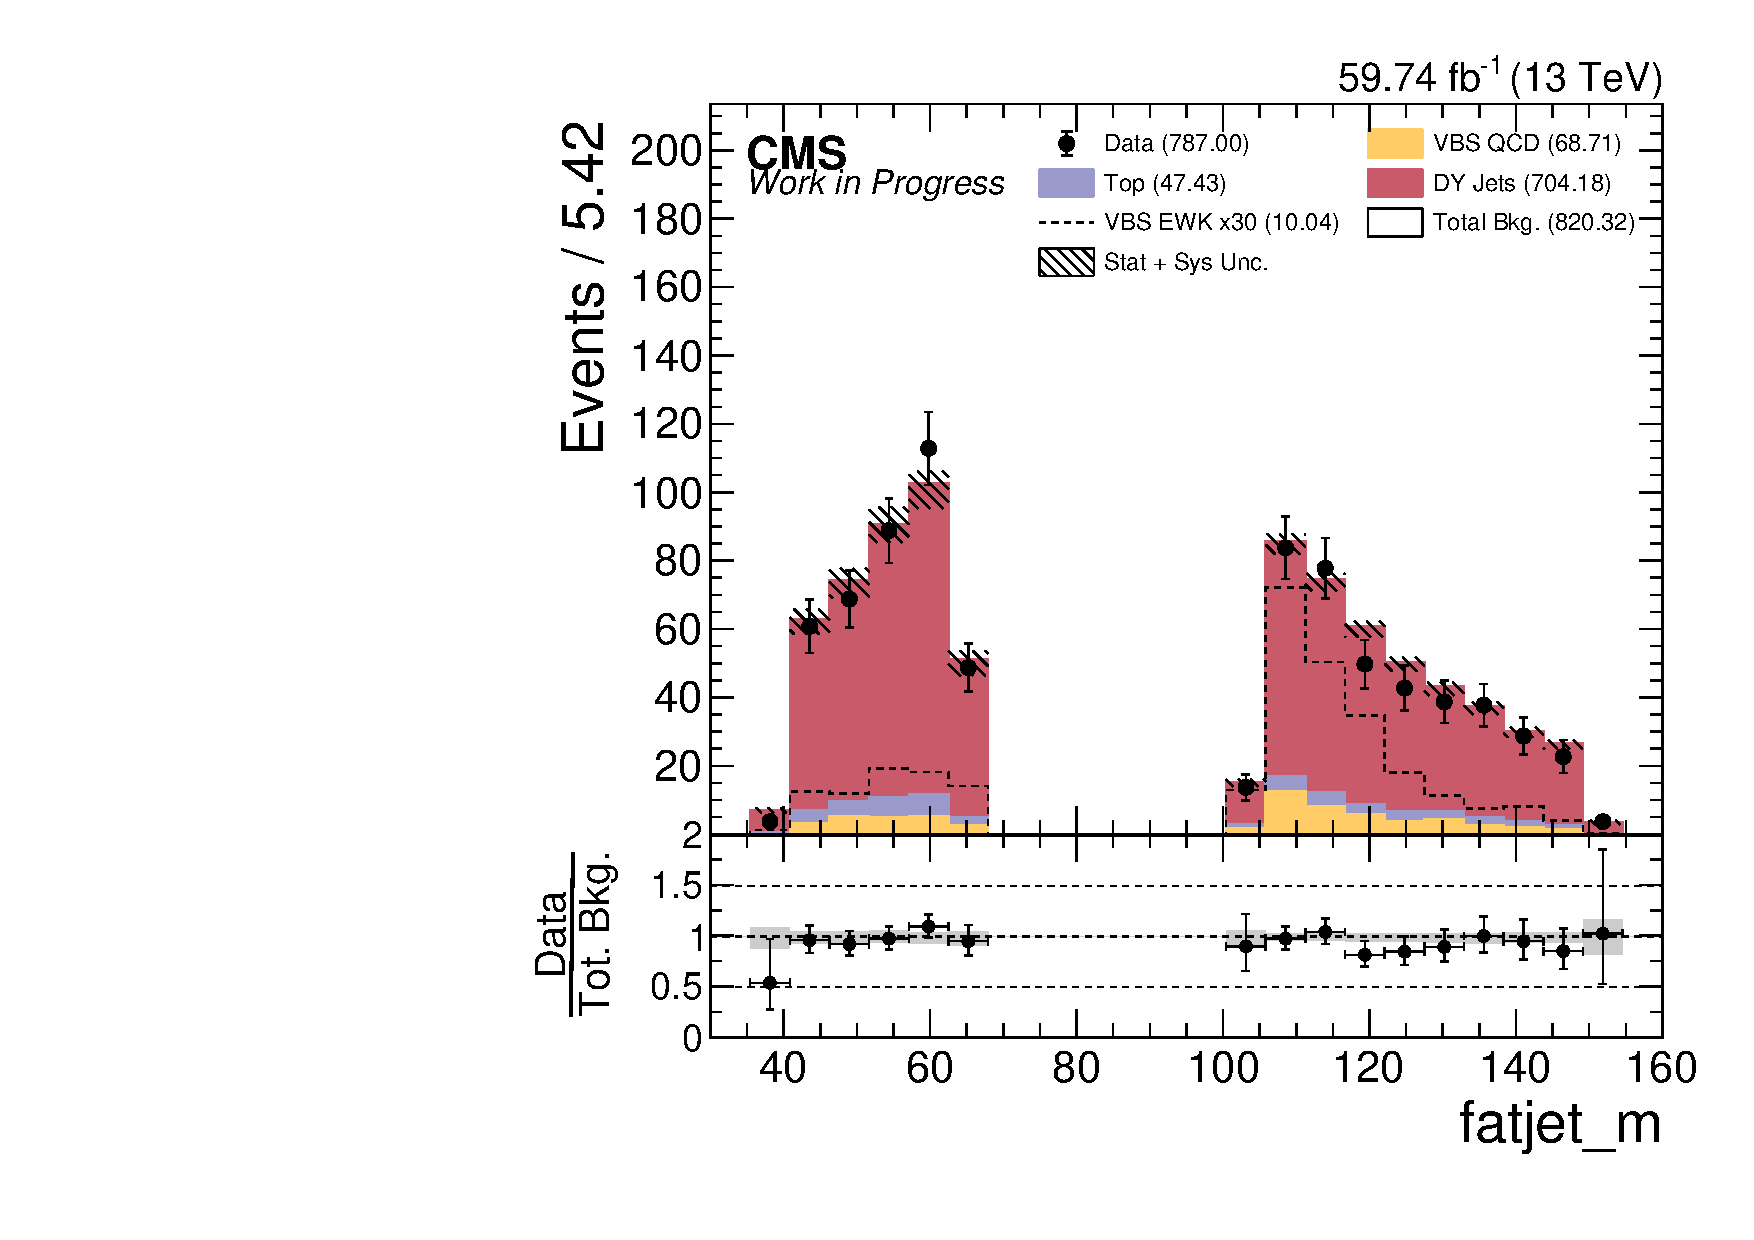
\includegraphics[width=0.30\textwidth]{analysis_plots/2018_zv/cr_vjets_l/fatjet_m.pdf} \\
  \caption[DY+Jets Control Region: Hadronic boson kinematics in Boosted ZV Channel]%
  {DY+Jets Control Region: Hadronic boson kinematics in Boosted ZV Channel. From Left to Right: 2016,
    2017, and 2018. From Top to Bottom: \( p_T \), \( \eta \), mass \( m \).}%
  \label{fig:zv-cr-vjets-l-fatjet-pt-eta-m}
\end{figure}

\begin{figure}[!ht]
  \centering
  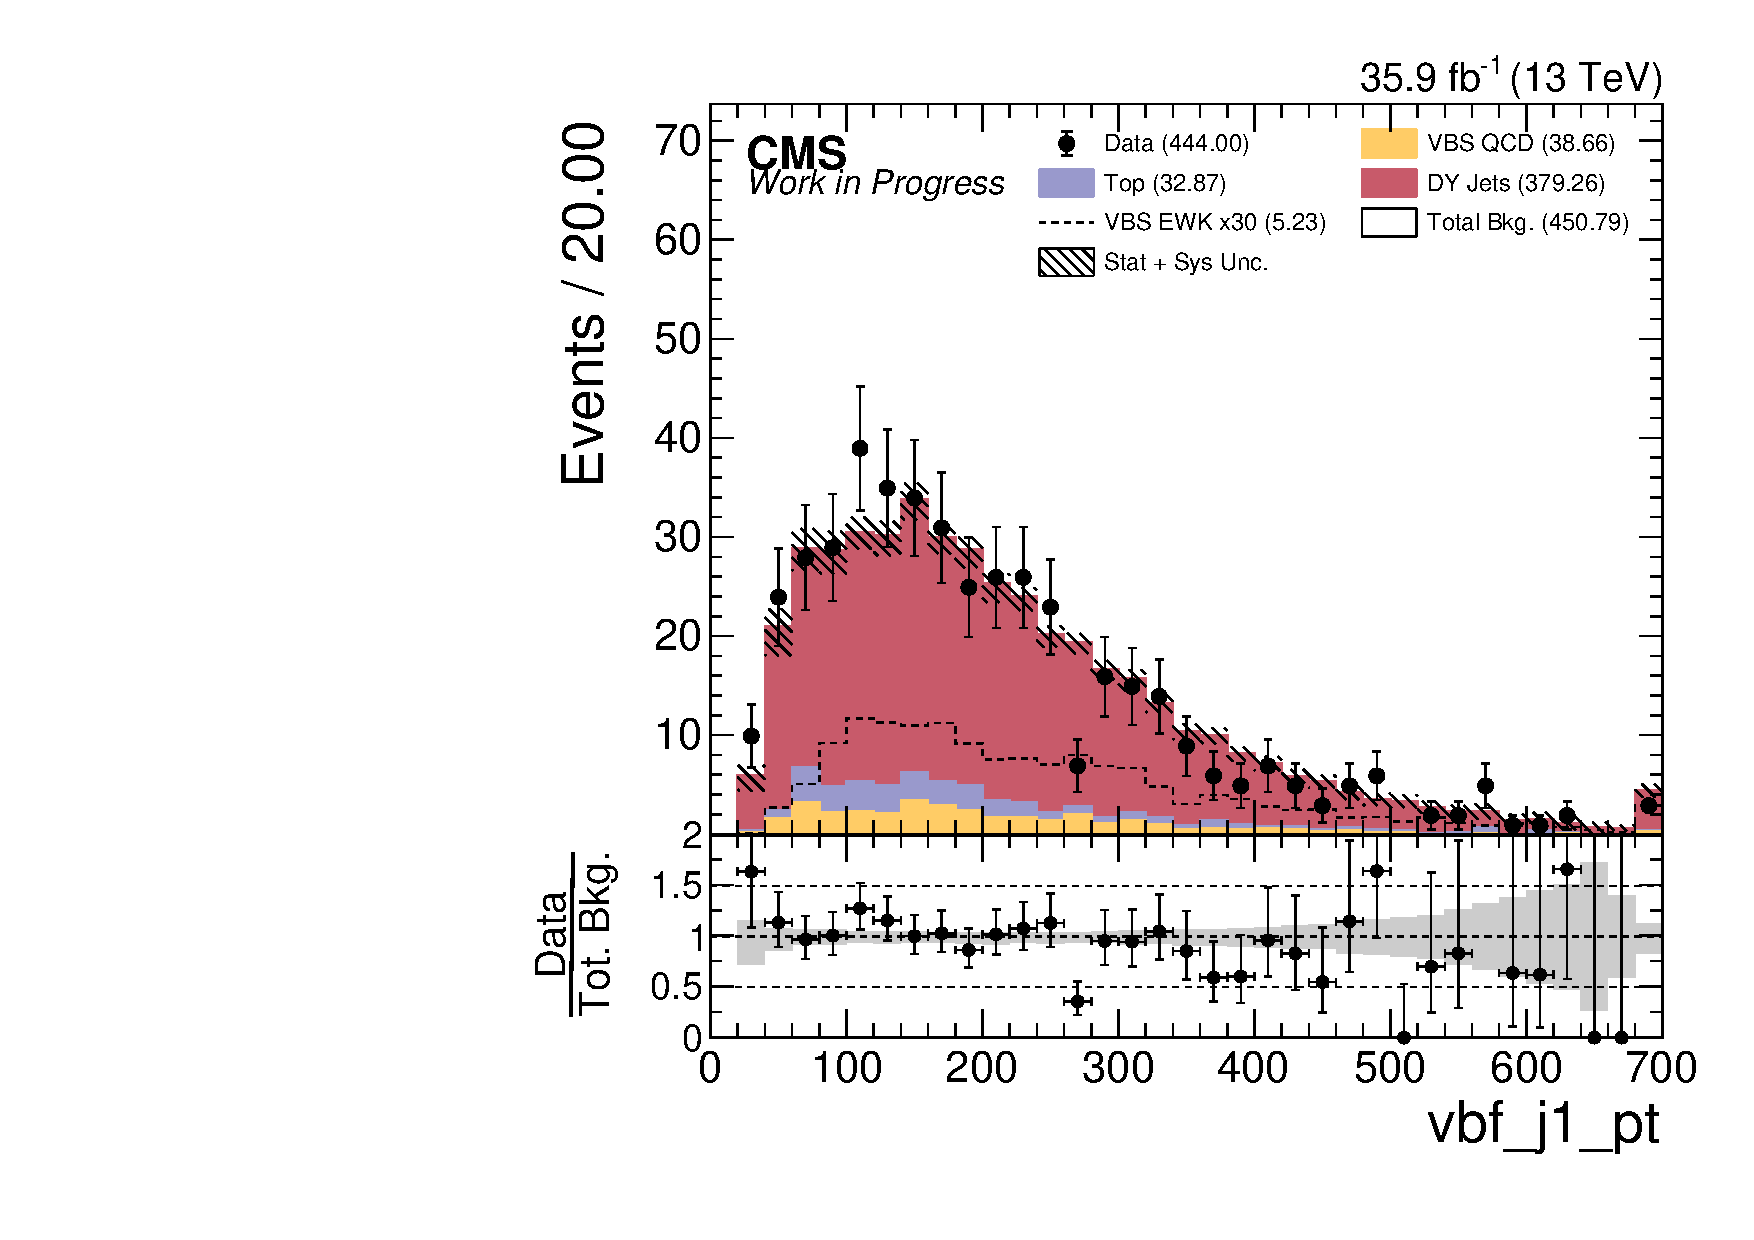
\includegraphics[width=0.30\textwidth]{analysis_plots/2016_zv/cr_vjets_l/vbf_j1_pt.pdf}
  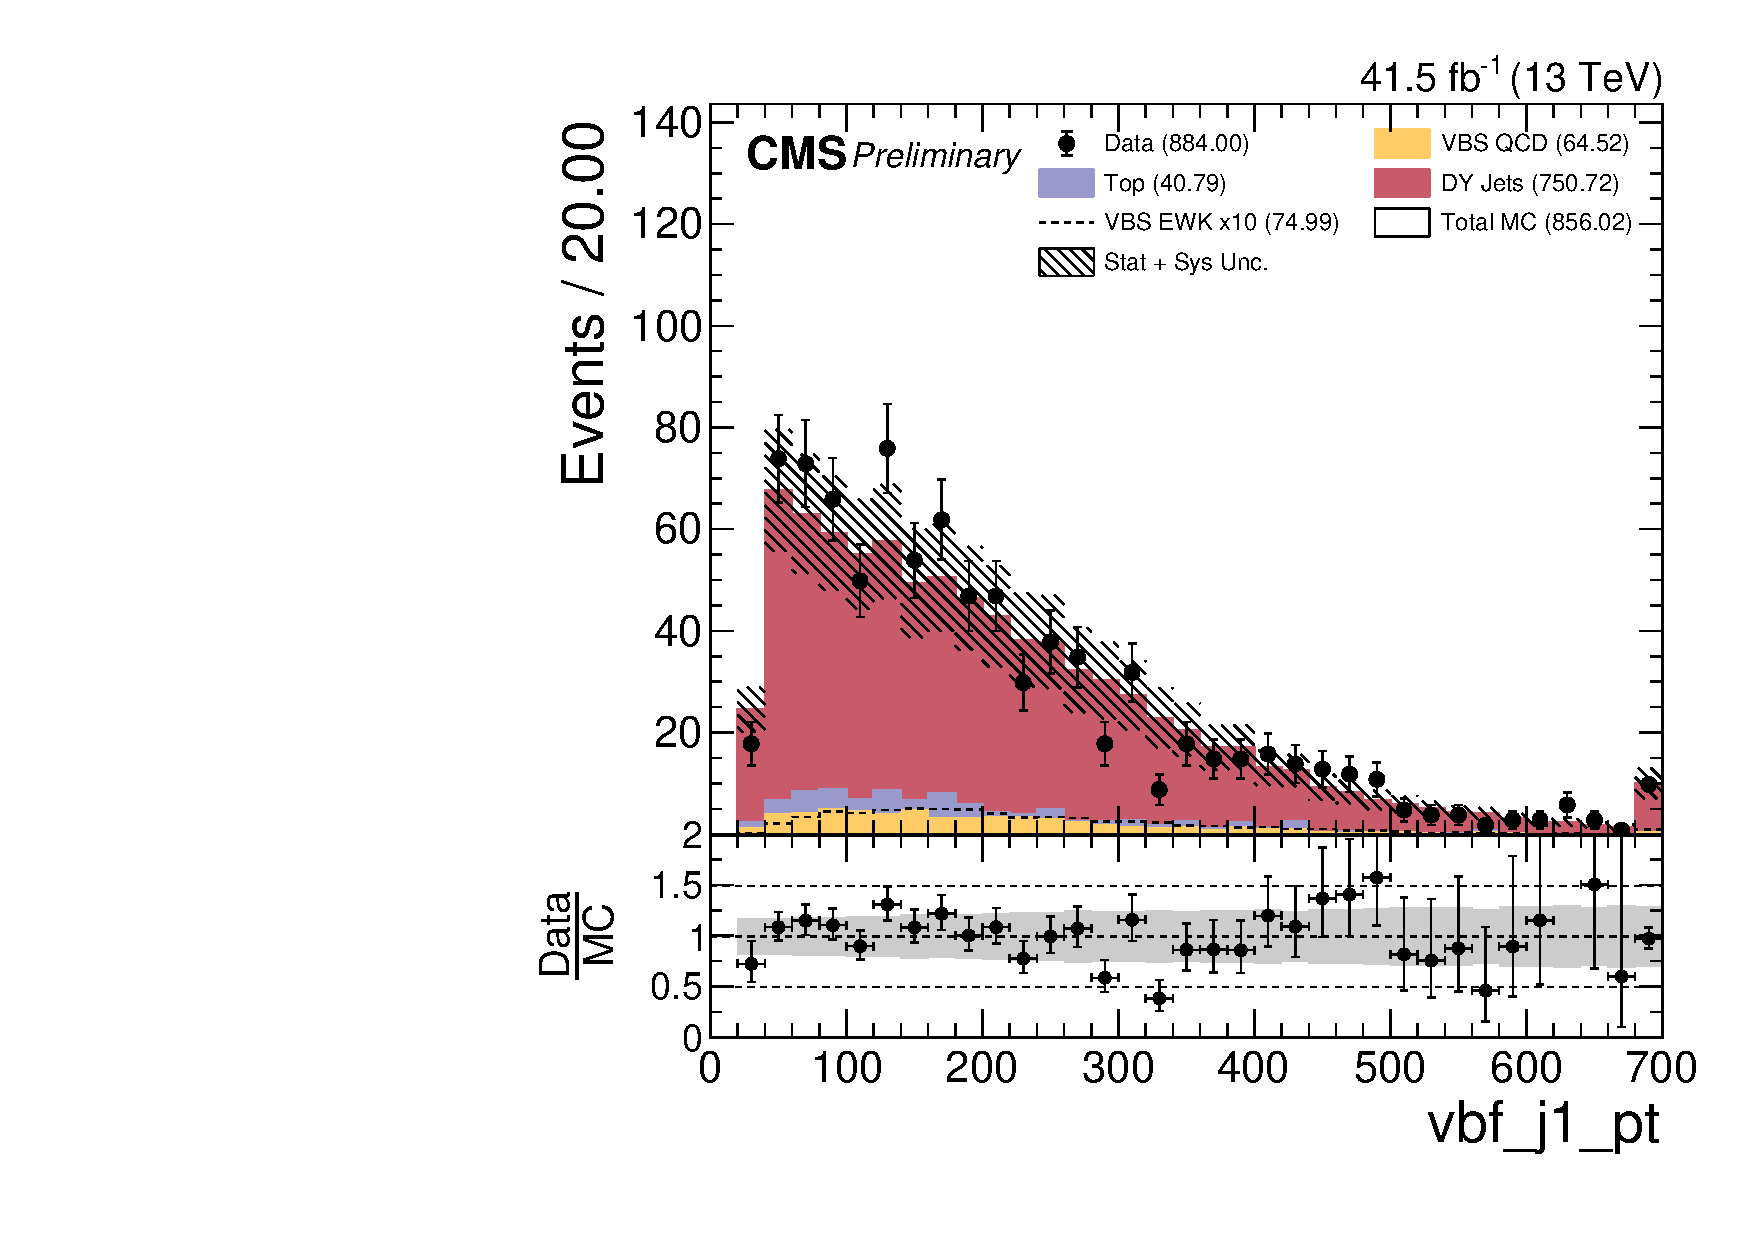
\includegraphics[width=0.30\textwidth]{analysis_plots/2017_zv/cr_vjets_l/vbf_j1_pt.pdf}
  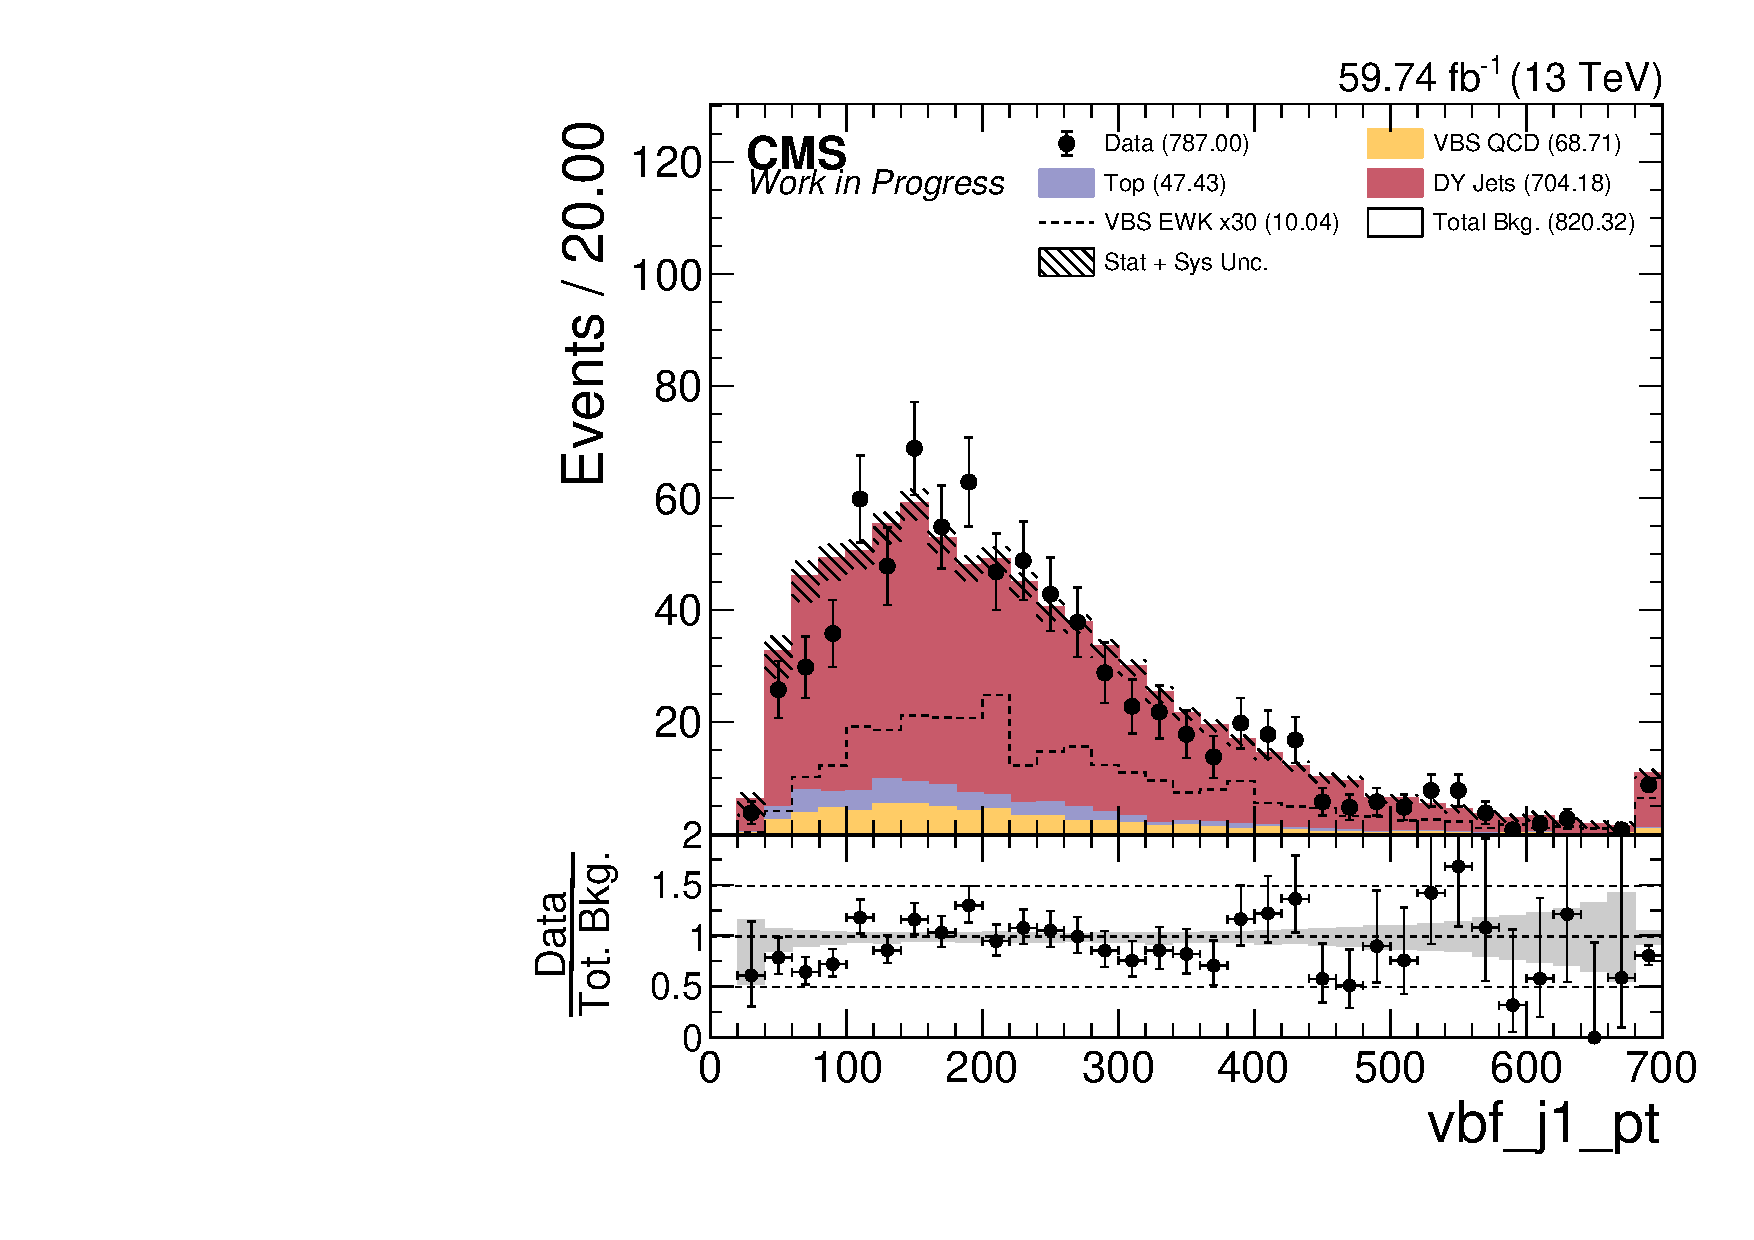
\includegraphics[width=0.30\textwidth]{analysis_plots/2018_zv/cr_vjets_l/vbf_j1_pt.pdf} \\
  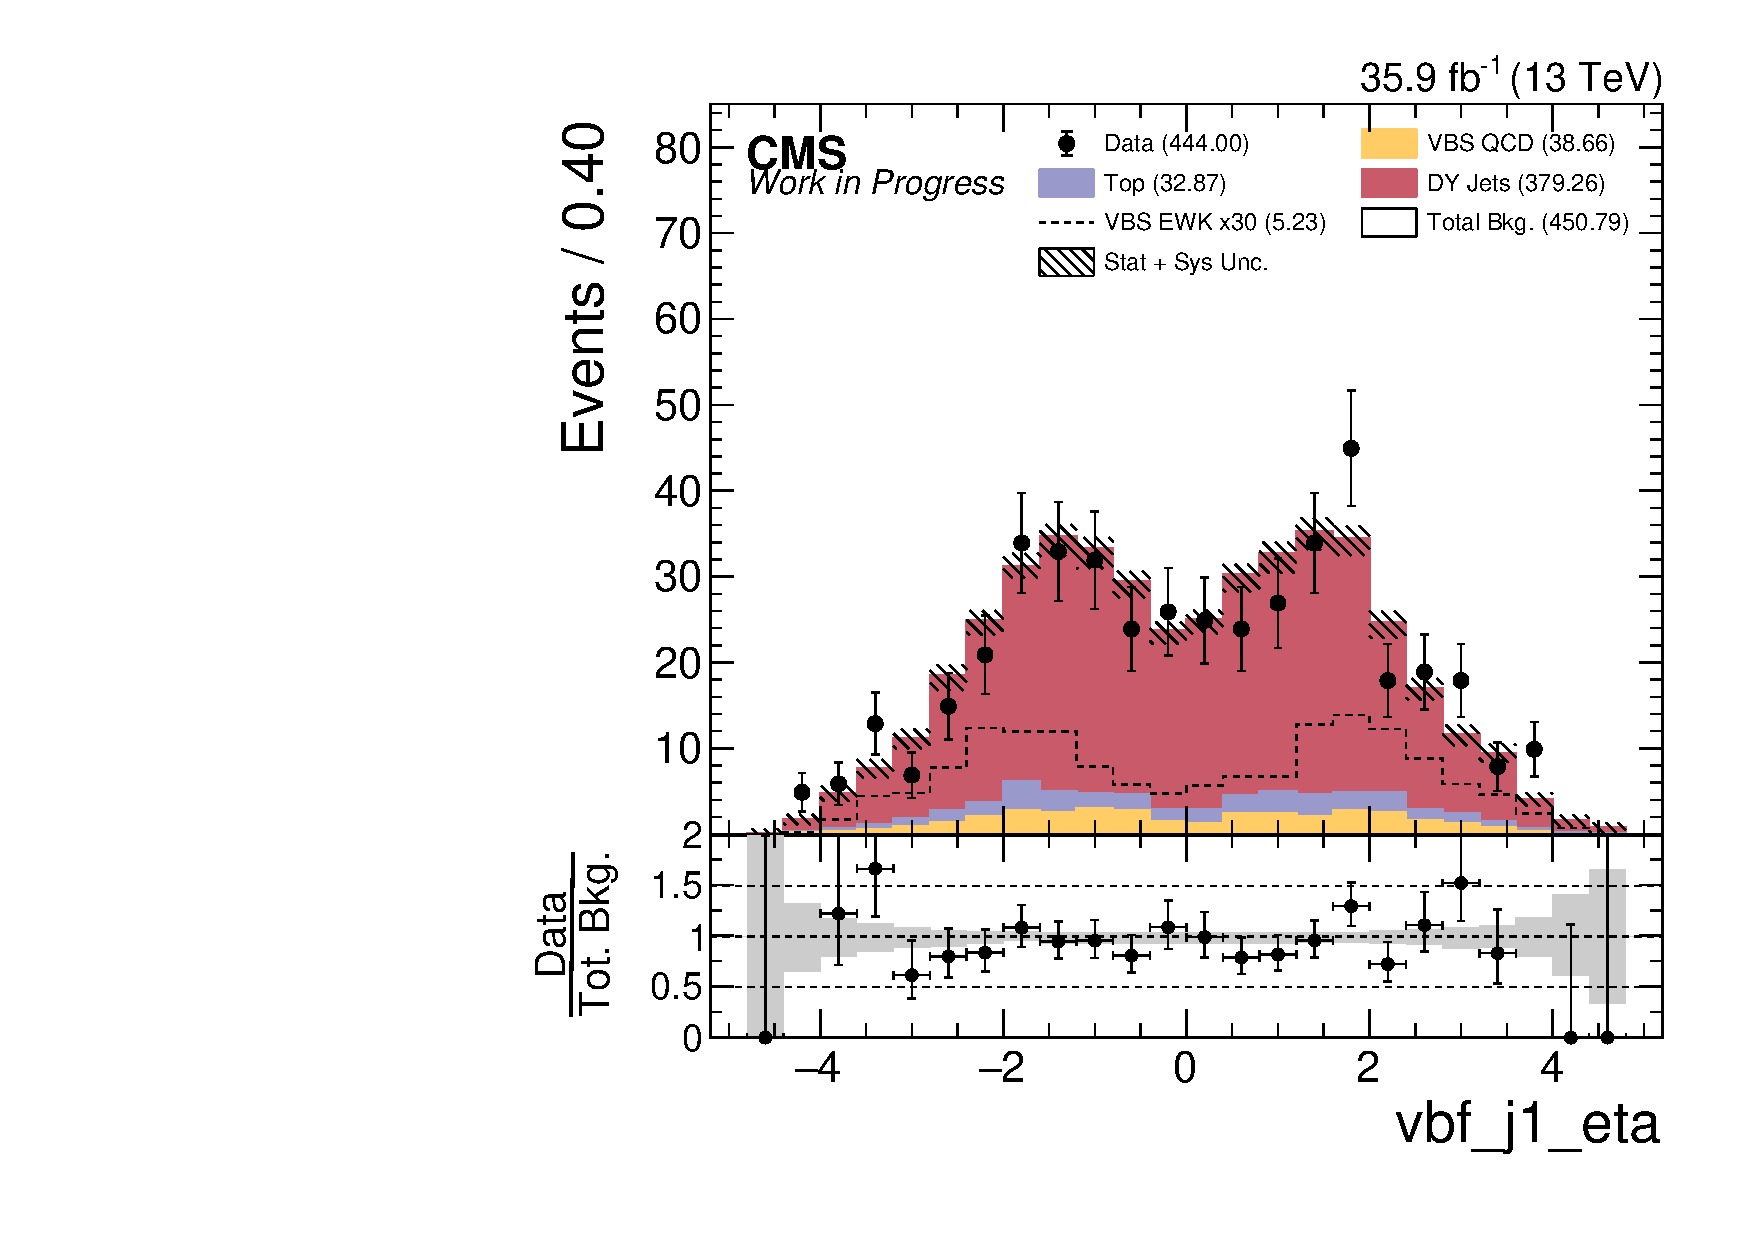
\includegraphics[width=0.30\textwidth]{analysis_plots/2016_zv/cr_vjets_l/vbf_j1_eta.pdf}
  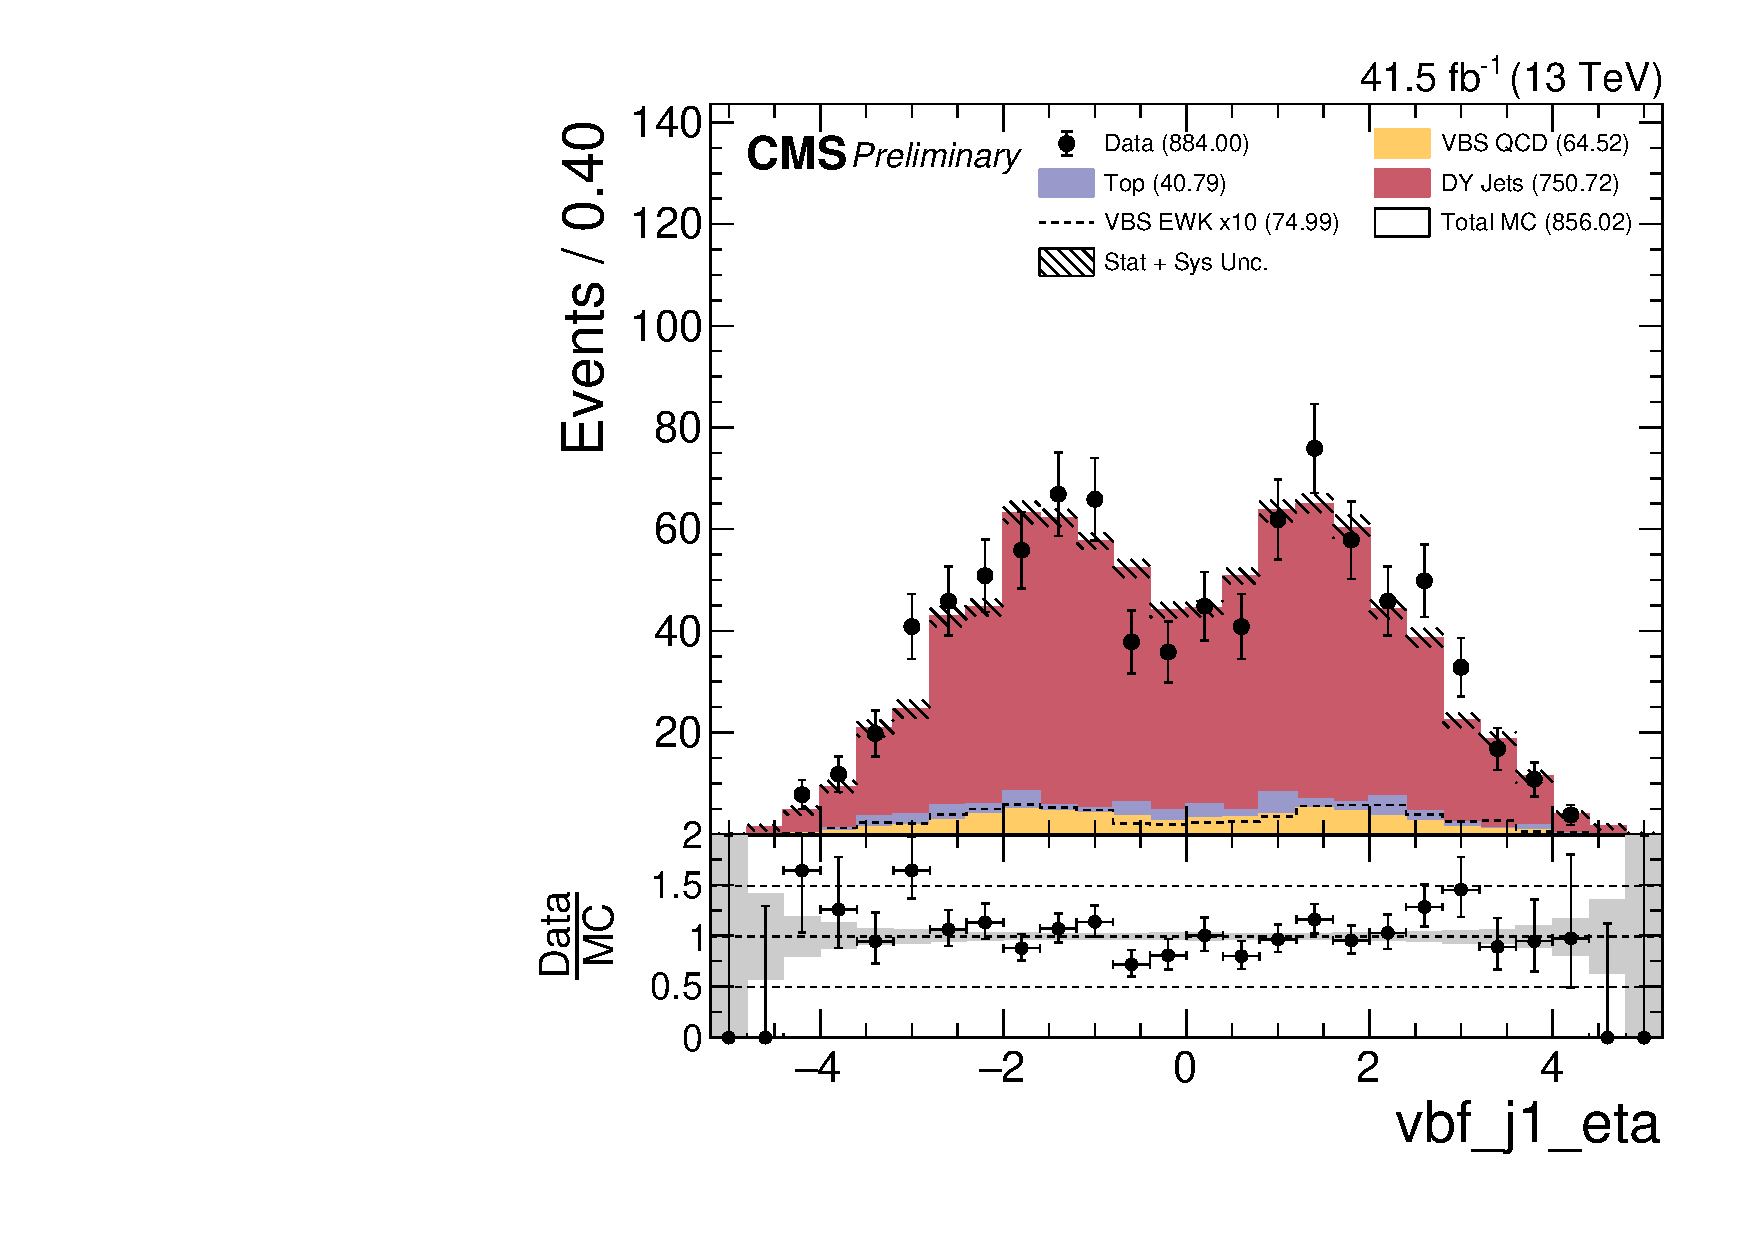
\includegraphics[width=0.30\textwidth]{analysis_plots/2017_zv/cr_vjets_l/vbf_j1_eta.pdf}
  \includegraphics[width=0.30\textwidth]{analysis_plots/2018_zv/cr_vjets_l/vbf_j1_eta.pdf} \\
  \includegraphics[width=0.30\textwidth]{analysis_plots/2016_zv/cr_vjets_l/vbf_j1_phi.pdf}
  \includegraphics[width=0.30\textwidth]{analysis_plots/2017_zv/cr_vjets_l/vbf_j1_phi.pdf}
  \includegraphics[width=0.30\textwidth]{analysis_plots/2018_zv/cr_vjets_l/vbf_j1_phi.pdf} \\
  \caption[DY+Jets Control Region: Leading VBS tagged jet kinematics in Boosted ZV Channel]%
  {DY+Jets Control Region: Leading VBS tagged jet kinematics in Boosted ZV Channel. From Left to Right: 2016,
    2017, and 2018. From Top to Bottom: \( p_T \), \( \eta \), \( \phi \).}%
  \label{fig:zv-cr-vjets-l-vbs1-pt-eta-m}
\end{figure}

\begin{figure}[!ht]
  \centering
  \includegraphics[width=0.30\textwidth]{analysis_plots/2016_zv/cr_vjets_l/vbf_j2_pt.pdf}
  \includegraphics[width=0.30\textwidth]{analysis_plots/2017_zv/cr_vjets_l/vbf_j2_pt.pdf}
  \includegraphics[width=0.30\textwidth]{analysis_plots/2018_zv/cr_vjets_l/vbf_j2_pt.pdf} \\
  \includegraphics[width=0.30\textwidth]{analysis_plots/2016_zv/cr_vjets_l/vbf_j2_eta.pdf}
  \includegraphics[width=0.30\textwidth]{analysis_plots/2017_zv/cr_vjets_l/vbf_j2_eta.pdf}
  \includegraphics[width=0.30\textwidth]{analysis_plots/2018_zv/cr_vjets_l/vbf_j2_eta.pdf} \\
  \includegraphics[width=0.30\textwidth]{analysis_plots/2016_zv/cr_vjets_l/vbf_j2_phi.pdf}
  \includegraphics[width=0.30\textwidth]{analysis_plots/2017_zv/cr_vjets_l/vbf_j2_phi.pdf}
  \includegraphics[width=0.30\textwidth]{analysis_plots/2018_zv/cr_vjets_l/vbf_j2_phi.pdf} \\
  \caption[DY+Jets Control Region: Trailing VBS tagged jet kinematics in Boosted ZV Channel]%
  {DY+Jets Control Region: Trailing VBS tagged jet kinematics in Boosted ZV Channel. From Left to Right: 2016,
    2017, and 2018. From Top to Bottom: \( p_T \), \( \eta \), \( \phi \).}%
  \label{fig:zv-cr-vjets-l-vbs2-pt-eta-m}
\end{figure}

\clearpage
\subsection{
  Resolved ZV DY+Jets Control Region
}

\begin{figure}[!ht]
  \centering
  \includegraphics[width=0.30\textwidth]{analysis_plots/2016_zjj/cr_vjets_e/lep1_pt.pdf}
  \includegraphics[width=0.30\textwidth]{analysis_plots/2017_zjj/cr_vjets_e/lep1_pt.pdf}
  \includegraphics[width=0.30\textwidth]{analysis_plots/2018_zjj/cr_vjets_e/lep1_pt.pdf} \\
  \includegraphics[width=0.30\textwidth]{analysis_plots/2016_zjj/cr_vjets_e/lep1_eta.pdf}
  \includegraphics[width=0.30\textwidth]{analysis_plots/2017_zjj/cr_vjets_e/lep1_eta.pdf}
  \includegraphics[width=0.30\textwidth]{analysis_plots/2018_zjj/cr_vjets_e/lep1_eta.pdf} \\
  \includegraphics[width=0.30\textwidth]{analysis_plots/2016_zjj/cr_vjets_e/lep1_phi.pdf}
  \includegraphics[width=0.30\textwidth]{analysis_plots/2017_zjj/cr_vjets_e/lep1_phi.pdf}
  \includegraphics[width=0.30\textwidth]{analysis_plots/2018_zjj/cr_vjets_e/lep1_phi.pdf} \\
  \caption[DY+Jets Control Region: Leading electron kinematics in Resolved ZV Channel]%
  {DY+Jets Control Region: Leading electron kinematics in Resolved ZV Channel. From Left to Right: 2016,
    2017, and 2018. From Top to Bottom: \( p_T \), \( \eta \), \( \phi \).}%
  \label{fig:zjj-cr-vjets-e-lep1-pt-eta-phi}
\end{figure}

\begin{figure}[!ht]
  \centering
  \includegraphics[width=0.30\textwidth]{analysis_plots/2016_zjj/cr_vjets_e/lep2_pt.pdf}
  \includegraphics[width=0.30\textwidth]{analysis_plots/2017_zjj/cr_vjets_e/lep2_pt.pdf}
  \includegraphics[width=0.30\textwidth]{analysis_plots/2018_zjj/cr_vjets_e/lep2_pt.pdf} \\
  \includegraphics[width=0.30\textwidth]{analysis_plots/2016_zjj/cr_vjets_e/lep2_eta.pdf}
  \includegraphics[width=0.30\textwidth]{analysis_plots/2017_zjj/cr_vjets_e/lep2_eta.pdf}
  \includegraphics[width=0.30\textwidth]{analysis_plots/2018_zjj/cr_vjets_e/lep2_eta.pdf} \\
  \includegraphics[width=0.30\textwidth]{analysis_plots/2016_zjj/cr_vjets_e/lep2_phi.pdf}
  \includegraphics[width=0.30\textwidth]{analysis_plots/2017_zjj/cr_vjets_e/lep2_phi.pdf}
  \includegraphics[width=0.30\textwidth]{analysis_plots/2018_zjj/cr_vjets_e/lep2_phi.pdf} \\
  \caption[DY+Jets Control Region: Trailing electron kinematics in Resolved ZV Channel]%
  {DY+Jets Control Region: Trailing electron kinematics in Resolved ZV Channel. From Left to Right: 2016,
    2017, and 2018. From Top to Bottom: \( p_T \), \( \eta \), \( \phi \).}%
  \label{fig:zjj-cr-vjets-e-lep2-pt-eta-phi}
\end{figure}

\begin{figure}[!ht]
  \centering
  \includegraphics[width=0.30\textwidth]{analysis_plots/2016_zjj/cr_vjets_m/lep1_pt.pdf}
  \includegraphics[width=0.30\textwidth]{analysis_plots/2017_zjj/cr_vjets_m/lep1_pt.pdf}
  \includegraphics[width=0.30\textwidth]{analysis_plots/2018_zjj/cr_vjets_m/lep1_pt.pdf} \\
  \includegraphics[width=0.30\textwidth]{analysis_plots/2016_zjj/cr_vjets_m/lep1_eta.pdf}
  \includegraphics[width=0.30\textwidth]{analysis_plots/2017_zjj/cr_vjets_m/lep1_eta.pdf}
  \includegraphics[width=0.30\textwidth]{analysis_plots/2018_zjj/cr_vjets_m/lep1_eta.pdf} \\
  \includegraphics[width=0.30\textwidth]{analysis_plots/2016_zjj/cr_vjets_m/lep1_phi.pdf}
  \includegraphics[width=0.30\textwidth]{analysis_plots/2017_zjj/cr_vjets_m/lep1_phi.pdf}
  \includegraphics[width=0.30\textwidth]{analysis_plots/2018_zjj/cr_vjets_m/lep1_phi.pdf} \\
  \caption[DY+Jets Control Region: Leading muon kinematics in Resolved ZV Channel]%
  {DY+Jets Control Region: Leading muon kinematics in Resolved ZV Channel. From Left to Right: 2016,
    2017, and 2018. From Top to Bottom: \( p_T \), \( \eta \), \( \phi \).}%
  \label{fig:zjj-cr-vjets-m-lep1-pt-eta-phi}
\end{figure}

\begin{figure}[!ht]
  \centering
  \includegraphics[width=0.30\textwidth]{analysis_plots/2016_zjj/cr_vjets_m/lep2_pt.pdf}
  \includegraphics[width=0.30\textwidth]{analysis_plots/2017_zjj/cr_vjets_m/lep2_pt.pdf}
  \includegraphics[width=0.30\textwidth]{analysis_plots/2018_zjj/cr_vjets_m/lep2_pt.pdf} \\
  \includegraphics[width=0.30\textwidth]{analysis_plots/2016_zjj/cr_vjets_m/lep2_eta.pdf}
  \includegraphics[width=0.30\textwidth]{analysis_plots/2017_zjj/cr_vjets_m/lep2_eta.pdf}
  \includegraphics[width=0.30\textwidth]{analysis_plots/2018_zjj/cr_vjets_m/lep2_eta.pdf} \\
  \includegraphics[width=0.30\textwidth]{analysis_plots/2016_zjj/cr_vjets_m/lep2_phi.pdf}
  \includegraphics[width=0.30\textwidth]{analysis_plots/2017_zjj/cr_vjets_m/lep2_phi.pdf}
  \includegraphics[width=0.30\textwidth]{analysis_plots/2018_zjj/cr_vjets_m/lep2_phi.pdf} \\
  \caption[DY+Jets Control Region: Trailing muon kinematics in Resolved ZV Channel]%
  {DY+Jets Control Region: Trailing muon kinematics in Resolved ZV Channel. From Left to Right: 2016,
    2017, and 2018. From Top to Bottom: \( p_T \), \( \eta \), \( \phi \).}%
  \label{fig:zjj-cr-vjets-m-lep2-pt-eta-phi}
\end{figure}

\begin{figure}[!ht]
  \centering
  \includegraphics[width=0.30\textwidth]{analysis_plots/2016_zjj/cr_vjets_l/dijet_j1_pt.pdf}
  \includegraphics[width=0.30\textwidth]{analysis_plots/2017_zjj/cr_vjets_l/dijet_j1_pt.pdf}
  \includegraphics[width=0.30\textwidth]{analysis_plots/2018_zjj/cr_vjets_l/dijet_j1_pt.pdf} \\
  \includegraphics[width=0.30\textwidth]{analysis_plots/2016_zjj/cr_vjets_l/dijet_j1_eta.pdf}
  \includegraphics[width=0.30\textwidth]{analysis_plots/2017_zjj/cr_vjets_l/dijet_j1_eta.pdf}
  \includegraphics[width=0.30\textwidth]{analysis_plots/2018_zjj/cr_vjets_l/dijet_j1_eta.pdf} \\
  \includegraphics[width=0.30\textwidth]{analysis_plots/2016_zjj/cr_vjets_l/dijet_m.pdf}
  \includegraphics[width=0.30\textwidth]{analysis_plots/2017_zjj/cr_vjets_l/dijet_m.pdf}
  \includegraphics[width=0.30\textwidth]{analysis_plots/2018_zjj/cr_vjets_l/dijet_m.pdf} \\
  \caption[DY+Jets Control Region: Hadronic boson leading jet kinematics in Resolved ZV Channel]%
  {DY+Jets Control Region: Hadronic boson leading jet kinematics in Resolved ZV Channel. From Left to Right: 2016,
    2017, and 2018. From Top to Bottom: \( p_T \), \( \eta \), invariant mass \( m_{jj} \).}%
  \label{fig:zjj-cr-vjets-l-dijet1-pt-eta-m}
\end{figure}

\begin{figure}[!ht]
  \centering
  \includegraphics[width=0.30\textwidth]{analysis_plots/2016_zjj/cr_vjets_l/dijet_j2_pt.pdf}
  \includegraphics[width=0.30\textwidth]{analysis_plots/2017_zjj/cr_vjets_l/dijet_j2_pt.pdf}
  \includegraphics[width=0.30\textwidth]{analysis_plots/2018_zjj/cr_vjets_l/dijet_j2_pt.pdf} \\
  \includegraphics[width=0.30\textwidth]{analysis_plots/2016_zjj/cr_vjets_l/dijet_j2_eta.pdf}
  \includegraphics[width=0.30\textwidth]{analysis_plots/2017_zjj/cr_vjets_l/dijet_j2_eta.pdf}
  \includegraphics[width=0.30\textwidth]{analysis_plots/2018_zjj/cr_vjets_l/dijet_j2_eta.pdf} \\
  \includegraphics[width=0.30\textwidth]{analysis_plots/2016_zjj/cr_vjets_l/dijet_m.pdf}
  \includegraphics[width=0.30\textwidth]{analysis_plots/2017_zjj/cr_vjets_l/dijet_m.pdf}
  \includegraphics[width=0.30\textwidth]{analysis_plots/2018_zjj/cr_vjets_l/dijet_m.pdf} \\
  \caption[DY+Jets Control Region: Hadronic boson trailing jet kinematics in Resolved ZV Channel]%
  {DY+Jets Control Region: Hadronic boson trailing jet kinematics in Resolved ZV Channel. From Left to Right: 2016,
    2017, and 2018. From Top to Bottom: \( p_T \), \( \eta \), invariant mass \( m_{jj} \).}%
  \label{fig:zjj-cr-vjets-l-dijet2-pt-eta-m}
\end{figure}

\begin{figure}[!ht]
  \centering
  \includegraphics[width=0.30\textwidth]{analysis_plots/2016_zjj/cr_vjets_l/vbf_j1_pt.pdf}
  \includegraphics[width=0.30\textwidth]{analysis_plots/2017_zjj/cr_vjets_l/vbf_j1_pt.pdf}
  \includegraphics[width=0.30\textwidth]{analysis_plots/2018_zjj/cr_vjets_l/vbf_j1_pt.pdf} \\
  \includegraphics[width=0.30\textwidth]{analysis_plots/2016_zjj/cr_vjets_l/vbf_j1_eta.pdf}
  \includegraphics[width=0.30\textwidth]{analysis_plots/2017_zjj/cr_vjets_l/vbf_j1_eta.pdf}
  \includegraphics[width=0.30\textwidth]{analysis_plots/2018_zjj/cr_vjets_l/vbf_j1_eta.pdf} \\
  \includegraphics[width=0.30\textwidth]{analysis_plots/2016_zjj/cr_vjets_l/vbf_j1_phi.pdf}
  \includegraphics[width=0.30\textwidth]{analysis_plots/2017_zjj/cr_vjets_l/vbf_j1_phi.pdf}
  \includegraphics[width=0.30\textwidth]{analysis_plots/2018_zjj/cr_vjets_l/vbf_j1_phi.pdf} \\
  \caption[DY+Jets Control Region: Leading VBS tagged jet kinematics in Resolved ZV Channel]%
  {DY+Jets Control Region: Leading VBS tagged jet kinematics in Resolved ZV Channel. From Left to Right: 2016,
    2017, and 2018. From Top to Bottom: \( p_T \), \( \eta \), \( \phi \).}%
  \label{fig:zjj-cr-vjets-l-vbs1-pt-eta-m}
\end{figure}

\begin{figure}[!ht]
  \centering
  \includegraphics[width=0.30\textwidth]{analysis_plots/2016_zjj/cr_vjets_l/vbf_j2_pt.pdf}
  \includegraphics[width=0.30\textwidth]{analysis_plots/2017_zjj/cr_vjets_l/vbf_j2_pt.pdf}
  \includegraphics[width=0.30\textwidth]{analysis_plots/2018_zjj/cr_vjets_l/vbf_j2_pt.pdf} \\
  \includegraphics[width=0.30\textwidth]{analysis_plots/2016_zjj/cr_vjets_l/vbf_j2_eta.pdf}
  \includegraphics[width=0.30\textwidth]{analysis_plots/2017_zjj/cr_vjets_l/vbf_j2_eta.pdf}
  \includegraphics[width=0.30\textwidth]{analysis_plots/2018_zjj/cr_vjets_l/vbf_j2_eta.pdf} \\
  \includegraphics[width=0.30\textwidth]{analysis_plots/2016_zjj/cr_vjets_l/vbf_j2_phi.pdf}
  \includegraphics[width=0.30\textwidth]{analysis_plots/2017_zjj/cr_vjets_l/vbf_j2_phi.pdf}
  \includegraphics[width=0.30\textwidth]{analysis_plots/2018_zjj/cr_vjets_l/vbf_j2_phi.pdf} \\
  \caption[DY+Jets Control Region: Trailing VBS tagged jet kinematics in Resolved ZV Channel]%
  {DY+Jets Control Region: Trailing VBS tagged jet kinematics in Resolved ZV Channel. From Left to Right: 2016,
    2017, and 2018. From Top to Bottom: \( p_T \), \( \eta \), \( \phi \).}%
  \label{fig:zjj-cr-vjets-l-vbs2-pt-eta-m}
\end{figure}

\clearpage
\section{
  Machine Learning Modeling
 }

Instead of traditional cut-based analysis, we decided to use \gls{MVA} a.k.a. \gls{ML}
technique to build a signal vs background classifier. The main reasoning behind using
a \gls{MVA} technique is so that we can build a model which can learn our
analysis topology from looser selection regions and still let us keep higher statistics
for final measurement.

\subsection{
  Algorithm: Gradient Boosted Decision Tree
}

Tools used \gls{TMVA} part of \ROOT{} package (FIXME reference). FIXME some details mathematical
details about BDT and specifically gradient BDT\@.

\subsection{
  Training and Results
}

Two models were trained for boosted and resolved topology and
the training was done using combined MC from all years 2016, 2017, 2018
to benefit from larger statistics see Table~\ref{tab:training-stats},
signal MC ``VBS\_EWK'' was trained against background ``DY + Jets LO'' since
that is dominant background in our analysis.
Each models \gls{BDT} hyper-parameters were tunned to prevent under and over-fitting,
and input variables used were also pruned in order of importance and keeping
model metrics \gls{AUC} of \gls{ROC} relatively unaffected. Distribution of final input variables
used in training are shown in Figure~\ref{fig:vbs-training-input-zv} and Figure~\ref{fig:vbs-training-input-zjj}.

\begin{table}[!ht]
  \centering
  \caption{Training and Testing Statistics}
  \begin{tabular}{lllll}%
    \toprule
             &            & \multicolumn{3}{c}{Number of Events}                    \\
    \cmidrule(lr){3-5}
    Channel  & Dataset    & Training                             & Testing & Total  \\
    \midrule
    Boosted  & Signal     & 7404                                 & 7405    & 14809  \\
    Boosted  & Background & 46991                                & 46991   & 93982  \\
    \midrule
    Resolved & Signal     & 23425                                & 23425   & 46850  \\
    Resolved & Background & 209368                               & 209368  & 418736 \\
    \bottomrule
  \end{tabular}\label{tab:training-stats}
\end{table}

\begin{figure}[!ht]
  \centering
  \includegraphics[width=0.4\textwidth]{analysis_plots/tmva_plots/zv_BDTG14_dibos_m.pdf}
  \includegraphics[width=0.4\textwidth]{analysis_plots/tmva_plots/zv_BDTG14_vbf_m.pdf} \\
  \includegraphics[width=0.4\textwidth]{analysis_plots/tmva_plots/zv_BDTG14_vbf1_AK4_qgid.pdf}
  \includegraphics[width=0.4\textwidth]{analysis_plots/tmva_plots/zv_BDTG14_vbf2_AK4_qgid.pdf} \\
  \includegraphics[width=0.4\textwidth]{analysis_plots/tmva_plots/zv_BDTG14_zeppLep_deta.pdf}
  \caption[Inputs Variables for training Boosted ZV BDT Classifier]%
  {Inputs Variables (combined for Run2 MC) for training Boosted ZV BDT Classifier.
    From top: Diboson invariant mass, VBS tagged jets invariant mass, \gls{QGL} of leading
    VBS tagged jet, \gls{QGL} of trailing VBS tagged jet, Zeppenfeld variable of leptonic boson.}%
  \label{fig:vbs-training-input-zv}
\end{figure}

\begin{figure}[!ht]
  \centering
  \includegraphics[width=0.32\textwidth]{analysis_plots/tmva_plots/zjj_BDTG14_dibos_m.pdf}
  \includegraphics[width=0.32\textwidth]{analysis_plots/tmva_plots/zjj_BDTG14_vbf_m.pdf} \\
  \includegraphics[width=0.32\textwidth]{analysis_plots/tmva_plots/zjj_BDTG14_ht_resolved.pdf}
  \includegraphics[width=0.32\textwidth]{analysis_plots/tmva_plots/zjj_BDTG14_lep2_eta.pdf} \\
  \includegraphics[width=0.32\textwidth]{analysis_plots/tmva_plots/zjj_BDTG14_vbf1_AK4_qgid.pdf}
  \includegraphics[width=0.32\textwidth]{analysis_plots/tmva_plots/zjj_BDTG14_vbf2_AK4_qgid.pdf}
  \includegraphics[width=0.32\textwidth]{analysis_plots/tmva_plots/zjj_BDTG14_zeppLep_deta.pdf}
  \caption[Inputs Variables for training Resolved ZV BDT Classifier]%
  {Inputs Variables (combined for Run2 MC) for training Resolved ZV BDT Classifier.
    From top: Diboson invariant mass, VBS tagged jets invariant mass,
    HT\textsuperscript{*} (\( p_{T} \) sum of jets), trailing lepton \( \eta \),
    \gls{QGL} of leading VBS tagged jet,
    \gls{QGL} of trailing VBS tagged jet, Zeppenfeld variable of leptonic boson.}%
  \label{fig:vbs-training-input-zjj}
\end{figure}

After training \gls{TMVA} \gls{BDT} evaluates input variables
and ranks them in terms of importance and separation
they provide in classification is listed in Table~\ref{tab:training-input-rank},
and the correlation matrix of variable is show in Figure~\ref{fig:vbs-training-correlation}.

\begin{table}[!ht]
  \centering
  \caption{Training Input Variable Ranking}
  \begin{tabular}{lllll}%
    \toprule
    Channel & Variable                   & Variable Name        & Importance & Separation \\
    \midrule
    \multirow{5}{*}{Boosted}
            & \( M_{JJ}^{VBS} \)         & \verb|vbf_m|         & 0.2496     & 0.1348     \\
            & Zeppenfeld \( Z_{V}^{*} \) & \verb|zeppLep_deta|  & 0.2396     & 0.1116     \\
            & QGL \( j_{1}^{VBS} \)      & \verb|vbf2_AK4_qgid| & 0.1889     & 0.02413    \\
            & QGL \( j_{2}^{VBS} \)      & \verb|vbf1_AK4_qgid| & 0.1780     & 0.02330    \\
            & \( M_{VV} \)               & \verb|dibos_m|       & 0.1439     & 0.005308   \\
    \midrule
    \multirow{7}{*}{Resolved}
            & Zeppenfeld \( Z_{V}^{*} \) & \verb|zeppLep_deta|  & 0.1955     & 0.1219     \\
            & \( M_{JJ}^{VBS} \)         & \verb|vbf_m|         & 0.1822     & 0.07998    \\
            & HT\textsuperscript{*}      & \verb|ht_resolved|   & 0.1693     & 0.04201    \\
            & QGL \( j_{1}^{VBS} \)      & \verb|vbf2_AK4_qgid| & 0.1403     & 0.02159    \\
            & QGL \( j_{2}^{VBS} \)      & \verb|vbf1_AK4_qgid| & 0.1341     & 0.03235    \\
            & \( M_{VV} \)               & \verb|dibos_m|       & 0.09098    & 0.01112    \\
            & \( \eta_{lep2} \)          & \verb|lep2_eta|      & 0.08760    & 0.01755    \\
    \bottomrule
  \end{tabular}\label{tab:training-input-rank}
\end{table}

\begin{figure}[!ht]
  \centering
  \includegraphics[width=0.4\textwidth]{analysis_plots/tmva_plots/zv_BDTG14_CorrelationMatrixS.pdf}
  \includegraphics[width=0.4\textwidth]{analysis_plots/tmva_plots/zjj_BDTG14_CorrelationMatrixS.pdf} \\
  \includegraphics[width=0.4\textwidth]{analysis_plots/tmva_plots/zv_BDTG14_CorrelationMatrixB.pdf}
  \includegraphics[width=0.4\textwidth]{analysis_plots/tmva_plots/zjj_BDTG14_CorrelationMatrixB.pdf} \\
  \caption[Correlation Matrix for Signal and Background]%
  {Correlation Matrix for Signal and Background. From Left to Right: Boosted, Resolved.
    From Top to Bottom: Signal, Background}%
  \label{fig:vbs-training-correlation}
\end{figure}

The under and over-fitting of trained model is checked by \gls{K-S} test
and \gls{ROC} curves comparison between training and testing datasets.
If the tests are not acceptable, then the training is redone with adjusted parameters.
The Figure~\ref{fig:vbs-training-score} show \gls{MVA} score and \gls{ROC} curves
of the BDT models. Models final metrics are listed in Table~\ref{tab:training-score}.

\begin{table}[!ht]
  \centering
  \caption{Models Metrics}
  \begin{tabular}{lc}%
    \toprule
    Channel  & AUC (\%) \\
    \midrule
    Boosted  & 78       \\
    \midrule
    Resolved & 79       \\
    \bottomrule
  \end{tabular}\label{tab:training-score}
\end{table}

\begin{figure}[!ht]
  \centering
  \includegraphics[width=0.4\textwidth]{analysis_plots/tmva_plots/zv_BDTG14.pdf}
  \includegraphics[width=0.4\textwidth]{analysis_plots/tmva_plots/zjj_BDTG14.pdf} \\
  \includegraphics[width=0.4\textwidth]{analysis_plots/tmva_plots/zv_BDTG14_roc.pdf}
  \includegraphics[width=0.4\textwidth]{analysis_plots/tmva_plots/zjj_BDTG14_roc.pdf}
  \caption[MVA Score ROC Curve]%
  {From Left to Right: Boosted, Resolved. Top to Bottom: MVA Score of BDT models,
    ROC Curves.}%
  \label{fig:vbs-training-score}
\end{figure}

\clearpage
\subsection{
  MVA Score inference in Signal Region
}

\begin{figure}[!ht]
  \centering
  \includegraphics[width=0.32\textwidth]{analysis_plots/2016_zv/sr_l/mva_score_zv_var2_log.pdf}
  \includegraphics[width=0.32\textwidth]{analysis_plots/2017_zv/sr_l/mva_score_zv_var2_log.pdf}
  \includegraphics[width=0.32\textwidth]{analysis_plots/2018_zv/sr_l/mva_score_zv_var2_log.pdf} \\
  \caption[MVA Score in Signal Region for Boosted ZV Channel]%
  {MVA Score in Signal Region for Boosted ZV Channel.}%
  \label{fig:zv-sr-l-mva-score}
\end{figure}

\begin{figure}[!ht]
  \centering
  \includegraphics[width=0.32\textwidth]{analysis_plots/2016_zjj/sr_l/mva_score_zjj_var2_log.pdf}
  \includegraphics[width=0.32\textwidth]{analysis_plots/2017_zjj/sr_l/mva_score_zjj_var2_log.pdf}
  \includegraphics[width=0.32\textwidth]{analysis_plots/2018_zjj/sr_l/mva_score_zjj_var2_log.pdf} \\
  \caption[MVA Score in Signal Region for Resolved ZV Channel]%
  {MVA Score in Signal Region for Resolved ZV Channel.}%
  \label{fig:zjj-sr-l-mva-score}
\end{figure}

\clearpage
\section{
  Measurement
 }

About \textsc{CombineLimit}\xspace used for calculating significance.

\subsection{
  Statistical and Systematic Uncertainties
}

\subsection{
  Significance
}

\begin{table}[!ht]
  \centering
  \caption{Significance}
  \begin{tabular}{lllll}%
    \toprule
    Channel  & 2016 & 2017 & 2018 & Combined \\
    \midrule
    Boosted  & 0.66 & 0.68 & 0.88 & 1.29     \\
    Resolved & 0.51 & 0.46 & 0.62 & 0.92     \\
    \midrule
    Combined &      &      &      & 1.59     \\
    \bottomrule
  \end{tabular}\label{tab:vbs-significance}
\end{table}

\clearpage
\subsection{
  Impact Plots
}
\begin{figure}[!ht]
  \centering
  \includegraphics[width=\textwidth,page=1]{analysis_plots/impact_plots/impacts_datacard_run2_z.pdf}
  \caption[Impact Plots]%
  {Impact Plots}%
  \label{fig:vbs-impact-plots-page1}
\end{figure}

\begin{figure}[!ht]
  \centering
  \includegraphics[width=\textwidth,page=2]{analysis_plots/impact_plots/impacts_datacard_run2_z.pdf}
  \caption[Impact Plots]%
  {Impact Plots}%
  \label{fig:vbs-impact-plots-page2}
\end{figure}

\begin{figure}[!ht]
  \centering
  \includegraphics[width=\textwidth,page=3]{analysis_plots/impact_plots/impacts_datacard_run2_z.pdf}
  \caption[Impact Plots]%
  {Impact Plots}%
  \label{fig:vbs-impact-plots-page3}
\end{figure}

\clearpage
\subsection{
  Postfit Plots
}

\begin{figure}[!ht]
  \centering
  \includegraphics[width=0.32\textwidth]{analysis_plots/2016_zv.sr_l_postfit/sr_l_postfit/mva_score_zv_var2_log.pdf}
  \includegraphics[width=0.32\textwidth]{analysis_plots/2017_zv.sr_l_postfit/sr_l_postfit/mva_score_zv_var2_log.pdf}
  \includegraphics[width=0.32\textwidth]{analysis_plots/2018_zv.sr_l_postfit/sr_l_postfit/mva_score_zv_var2_log.pdf} \\
  \caption[MVA Score postfit in Signal Region for Boosted ZV Channel]%
  {(Asimov Data) MVA Score postfit in Signal Region for Boosted ZV Channel.}%
  \label{fig:zv-sr-l-mva-score-postfit}
\end{figure}

\begin{figure}[!ht]
  \centering
  \includegraphics[width=0.32\textwidth]{analysis_plots/2016_zjj.sr_l_postfit/sr_l_postfit/mva_score_zjj_var2_log.pdf}
  \includegraphics[width=0.32\textwidth]{analysis_plots/2017_zjj.sr_l_postfit/sr_l_postfit/mva_score_zjj_var2_log.pdf}
  \includegraphics[width=0.32\textwidth]{analysis_plots/2018_zjj.sr_l_postfit/sr_l_postfit/mva_score_zjj_var2_log.pdf} \\
  \caption[MVA Score postfit in Signal Region for Resolved ZV Channel]%
  {(Asimov Data) MVA Score postfit in Signal Region for Resolved ZV Channel. (Asimov Data)}%
  \label{fig:zjj-sr-l-mva-score-postfit}
\end{figure}